\documentclass{article}

\usepackage{float}
\usepackage{geometry}
\usepackage{fancyhdr}
\usepackage{graphicx}
\usepackage{amsmath}
\usepackage{amsfonts}
\usepackage{amssymb}
\usepackage{amsthm}
\usepackage[utf8]{inputenc}
\usepackage[T1]{fontenc}
\usepackage[french]{babel}
\usepackage{libertine}
\usepackage{listings}
\usepackage{color}
\usepackage[table]{xcolor}
\usepackage{minted}
\usepackage{multicol}
\usepackage{csquotes}
\usepackage[hyphens]{url}
\usepackage{hyperref}
\usepackage[center]{caption}
\usepackage[backend=biber, style=alphabetic, sorting=ynt, block=ragged]{biblatex}
\addbibresource{references.bib}
\setminted{frame=lines,
    framesep=2mm,
    baselinestretch=1.2,
    fontsize=\footnotesize,
    linenos,
    breaklines
}
\hypersetup{
    colorlinks=true,
    pdftitle={PFE - Pluie en Australie},
    breaklinks = true
}
    
\begin{document}

\newcommand{\HRule}{\rule{\linewidth}{0.5mm}}

\begin{titlepage}
  \begin{sffamily}
  \begin{center}
    \hfill
    
\includegraphics[scale=0.06]{./Images/logoINSARouen.png}~\\[1.5cm]

    \textsc{\LARGE INSA ROUEN}\\[1cm]

    \textsc{\Large Projet de Fin d'Études}\\[1cm]

    \HRule \\[0.4cm]
    { \huge \bfseries Pluie en Australie\\[0.4cm] }

    \HRule \\[1cm]
    %\includegraphics[width=0.7\textwidth]{Ressources/front.pdf}
    %\\[1cm]

    \begin{minipage}{0.4\textwidth}
      \begin{flushleft} \large
        Théophile THIERRY\\
      \end{flushleft}
    \end{minipage}
    \begin{minipage}{0.4\textwidth}
      \begin{flushright} \large
        \textsc{M. PORTIER}\\
         2021-2022\\
      \end{flushright}
    \end{minipage}

    \vfill

  \end{center}
  \end{sffamily}
\end{titlepage}

\newpage

\tableofcontents
\listoffigures
\listoftables
\newpage

\part{Introduction}
Ce projet a été réalisé dans le cadre du PFE (Projet de Fin d'Études), réalisé en 5ème année de la formation de Génie Mathématique à l'INSA Rouen Normandie. Le sujet de ce projet est : "Utilisation d’algorithmes de machines learning pour la résolution d’un challenge Kaggle". Il est encadré par M. Bruno Portier.  

La base de données Kaggle choisie ici est "Rain in Australia", qui regroupe des informations gouvernementales sur la météo en Australie. Le but de ce "challenge" est de réaliser un algorithme de machine learning pour prédire s'il pleut le lendemain d'une journée donnée. 

Nous décrirons dans un premier temps la base de données et, dans un espoir de la connaître un peu mieux, nous analyserons les liens et corrélations entre ses variables. Ensuite, après avoir mis en œuvre des outils de complétion des données, nous pourrons construire nos modèles de prédiction et les comparer pour choisir le plus adapté dans notre cas. 

\newpage
\part{Description des données}

\section{Présentation des données}

Les données utilisées pour ce projet peuvent être trouvées sur le site \href{https://www.kaggle.com/jsphyg/weather-dataset-rattle-package}{Kaggle}. Elles ont été récupérées des données du gouvernement australien, dans la partie \href{http://www.bom.gov.au/climate/dwo}{Daily Weather Observations}, et ont été complétées avec les données de la partie  \href{http://www.bom.gov.au/climate/data}{Climate Data Online}.

Ces données contiennent 10 ans d'observations de la météo australienne sur 49 lieux différents entre 2007 et 2017. Une observation est constituée de toutes ces variables : 

\begin{itemize}
    \item Date : date de la mesure.
    \item Location : localisation de la mesure.
    \item MinTemp : température minimale dans les 24h jusqu'à 9h du matin (en °C).
    \item MaxTemp : température maximale dans les 24h jusqu'à 9h du matin (en °C).
    \item Rainfall : précipitation dans les 24h jusqu'à 9h du matin (en mm).
    \item Evaporation : mesure prise sur un bac d'évaporation de classe A dans les 24h jusqu'à 9h du matin (en mm).
    \item Sunshine : ensoleillement en heure dans les 24h jusqu'à minuit.
    \item WindGustDir : direction de la plus forte rafale dans les 24 heures jusqu'à minuit (16 points cardinaux/intercardinaux).   
    \item WindGustSpeed : vitesse de la plus forte rafale dans les 24 heures jusqu'à minuit (16 points cardinaux/intercardinaux).
    \item WindDir9am : direction du vent à 9h du matin.
    \item WindDir3pm : idem à 15h.
    \item WindSpeed9am : vitesse du vent à 9h.
    \item WindSpeed3pm : idem à 15h.
    \item Humidity9am : taux d'humidité relative à 9h.
    \item Humidity3pm : idem à 15h.
    \item Pressure9am : pression atmosphérique réduite au niveau moyen de la mer à 9h.
    \item Pressure3pm : idem à 15h.
    \item Cloud9am : fraction du ciel couverte par un nuage à 9h (en huitième).   
    \item Cloud3pm : idem à 15h.
    \item Temp9am : température à 9h (en °C).
    \item Temp3pm : idem à 15h.
    \item RainToday : s'il a plu le jour même.
    \item RainTomorrow : s'il a plu le lendemain.   
\end{itemize}
Jetons tout d'abord un coup d'œil aux variables numériques de nos données. 

\subsection{Variables numériques}

\begin{table}[H]
    \centering
    \resizebox{\textwidth}{!}{
        \begin{tabular}{|r||rrrrrrrr|}
            \hline
            & Min. & 1st Qu. & Median & Mean & 3rd Qu. & Max. & NA's & Std. \\ 
            \hline
            \hline
            MinTemp & -8.50 & 7.60 & 12.00 & 12.19 & 16.90 & 33.90 & 1485.00 & 6.40 \\ 
            MaxTemp & -4.80 & 17.90 & 22.60 & 23.22 & 28.20 & 48.10 & 1261.00 & 7.12 \\ 
            Rainfall & 0.00 & 0.00 & 0.00 & 2.36 & 0.80 & 371.00 & 3261.00 & 8.48 \\ 
            Evaporation & 0.00 & 2.60 & 4.80 & 5.47 & 7.40 & 145.00 & 62790.00 & 4.19 \\ 
            Sunshine & 0.00 & 4.80 & 8.40 & 7.61 & 10.60 & 14.50 & 69835.00 & 3.79 \\ 
            WindGustSpeed & 6.00 & 31.00 & 39.00 & 40.04 & 48.00 & 135.00 & 10263.00 & 13.61 \\ 
            WindSpeed9am & 0.00 & 7.00 & 13.00 & 14.04 & 19.00 & 130.00 & 1767.00 & 8.92 \\ 
            WindSpeed3pm & 0.00 & 13.00 & 19.00 & 18.66 & 24.00 & 87.00 & 3062.00 & 8.81 \\ 
            Humidity9am & 0.00 & 57.00 & 70.00 & 68.88 & 83.00 & 100.00 & 2654.00 & 19.03 \\ 
            Humidity3pm & 0.00 & 37.00 & 52.00 & 51.54 & 66.00 & 100.00 & 4507.00 & 20.80 \\ 
            Pressure9am & 980.50 & 1012.90 & 1017.60 & 1017.65 & 1022.40 & 1041.00 & 15065.00 & 7.11 \\ 
            Pressure3pm & 977.10 & 1010.40 & 1015.20 & 1015.26 & 1020.00 & 1039.60 & 15028.00 & 7.04 \\ 
            Cloud9am & 0.00 & 1.00 & 5.00 & 4.45 & 7.00 & 9.00 & 55888.00 & 2.89 \\ 
            Cloud3pm & 0.00 & 2.00 & 5.00 & 4.51 & 7.00 & 9.00 & 59358.00 & 2.72 \\ 
            Temp9am & -7.20 & 12.30 & 16.70 & 16.99 & 21.60 & 40.20 & 1767.00 & 6.49 \\ 
            Temp3pm & -5.40 & 16.60 & 21.10 & 21.68 & 26.40 & 46.70 & 3609.00 & 6.94 \\ 
                \hline
        \end{tabular}
    }
    \caption{Résumé des variables numériques}
    \label{table:summary}
\end{table}

Comme nous pouvons le constater dans la Table \ref{table:summary}, il manque, pour certaines variables numériques, beaucoup d'observations (voir la colonne \emph{NA's}), et principalement sur les variables \emph{Sunshine}, \emph{Evaporation}, \emph{Cloud9am} et \emph{Cloud3pm}, dont nous avons moins de 60\% des observations. Nous verrons en quoi cela comporte un problème pour notre objectif et comment nous pourrons y remédier.

Nous pouvons de plus noter certaines choses : les variables à 9h et 15h sont très similaire, et il fait évidemment plus chaud l'après-midi que le matin, il y a aussi en moyenne plus de vent et moins d'humidité. 

Globalement, ce tableau nous permet de nous rendre compte des distributions de chacune des variables et de leur ordre de grandeur. 

\subsection{Variables factorielles}

\begin{figure}[htp]
    \centering
    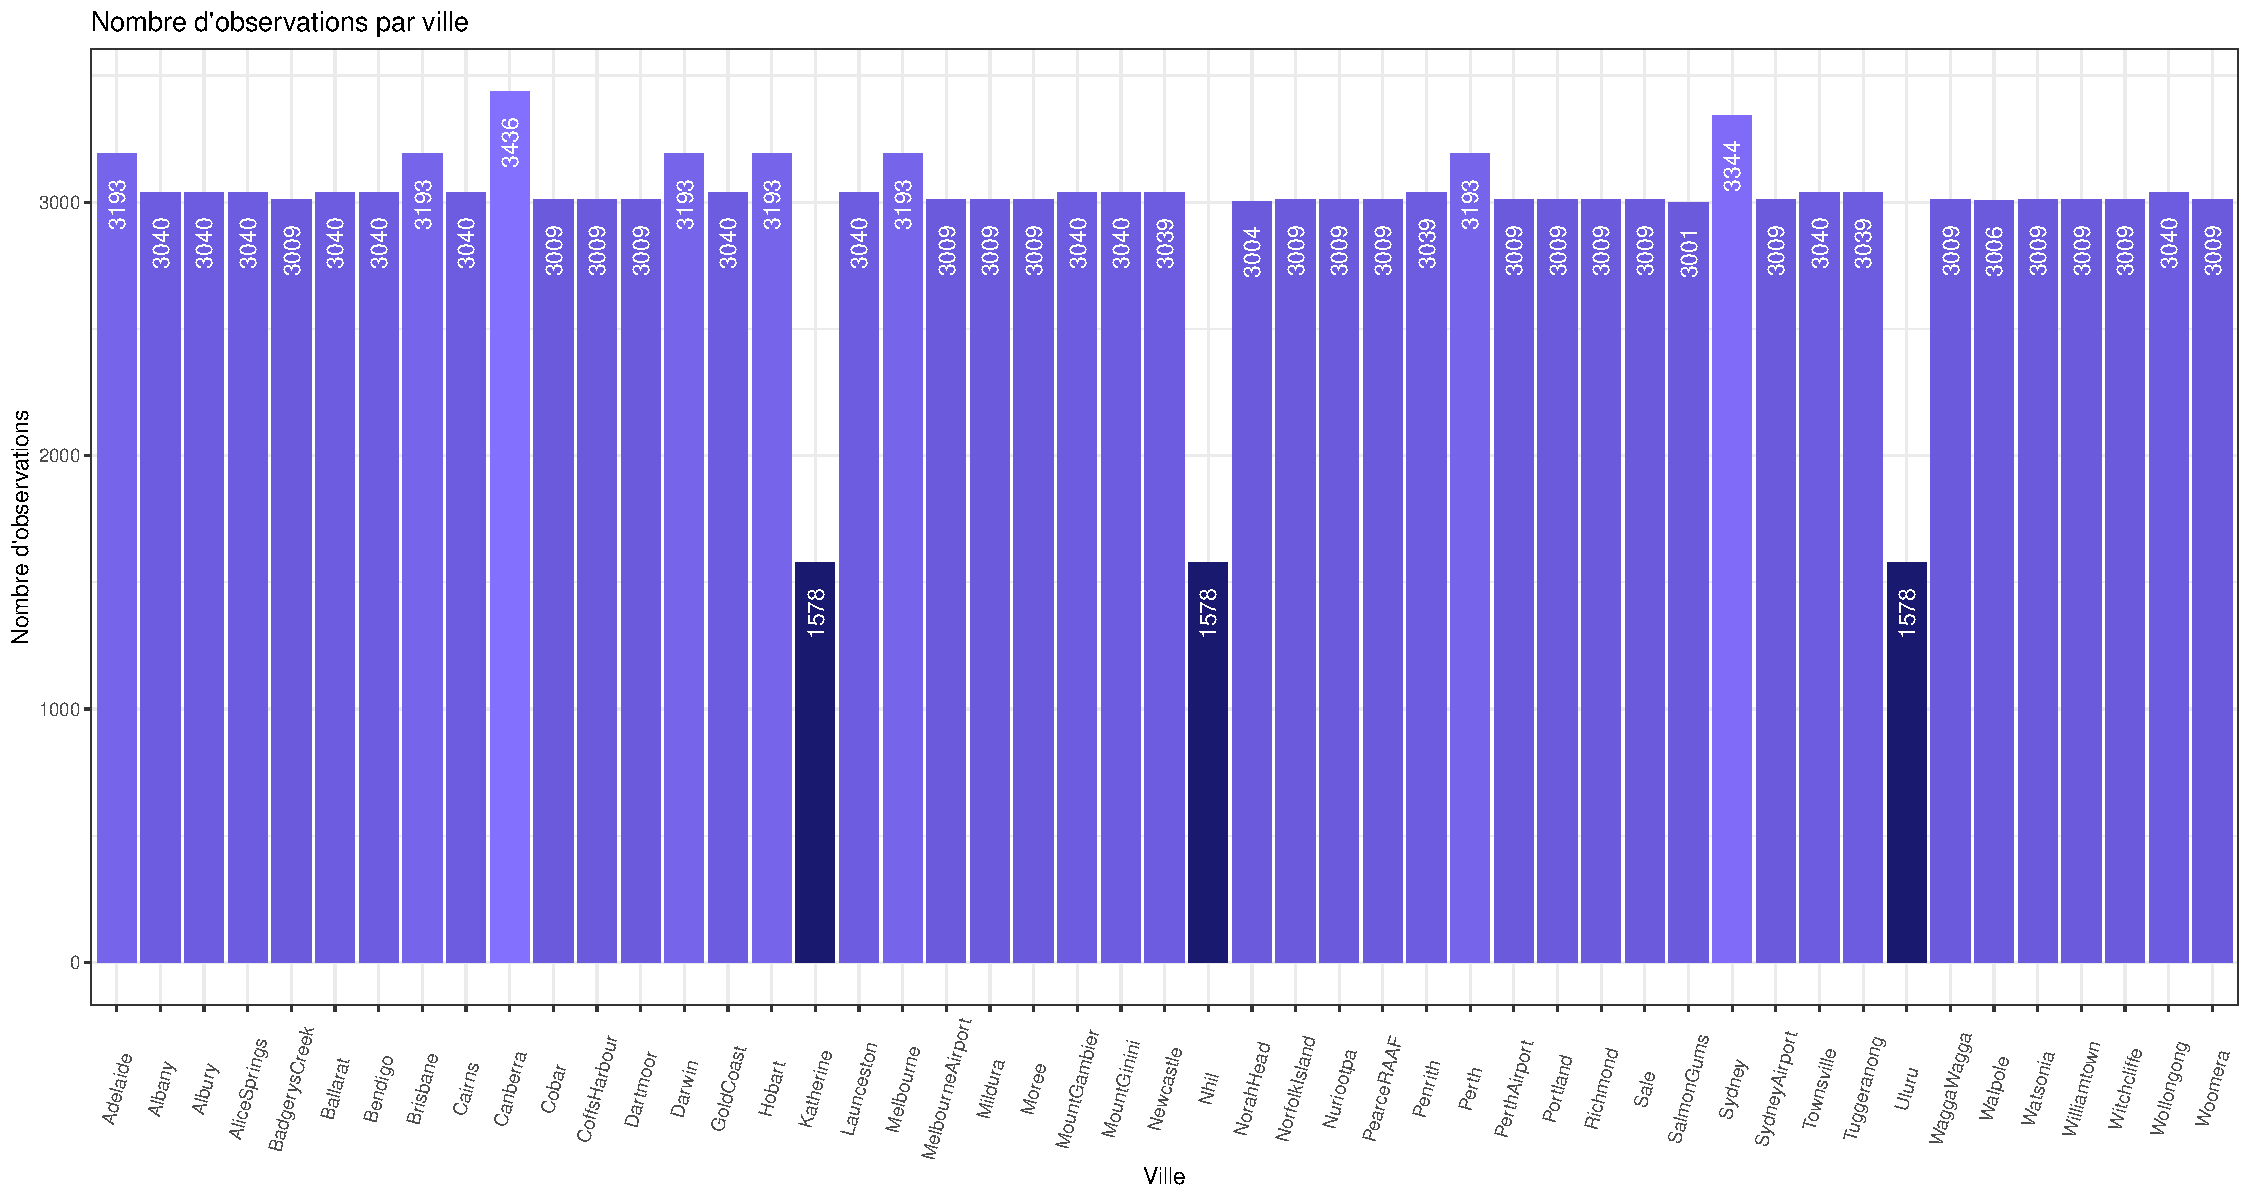
\includegraphics[width=\textwidth]{Images/hist_observations_cities.pdf}
    \caption{Nombre d'observations pour chaque ville}
    \label{fig:obs_per_cities}
\end{figure}

Regardons désormais les variables avec des facteurs. Les dates, tout d'abord, vont du 2007-11-01 au 2017-06-25, ce qui représente 3524 jours. Si l'on regarde la distribution du nombre d'observations par lieux observés, on devrait donc voir que chacune d'entre elles en ont 3524 (voir Figure \ref{fig:obs_per_cities}). On voit déjà qu'il manque certaines dates d'observations pour la plupart des villes, et pour 3 d'entre elles (Katherine, Nhil et Uluru) nous en avons moins de la moitié. En effet, dans ces endroits là les observations n'ont commenées qu'en 2013.

Penchons-nous désormais sur les variables de direction du vent en regardant la distribution de leurs facteurs dans les Tables \ref{table:wind_gust_dir}, \ref{table:wind_dir_9am} et \ref{table:wind_dir_3pm}.

\begin{table}[htp]
    \centering
    \resizebox{\textwidth}{!}{
        \begin{tabular}{|r||*{17}{r}|}
            \hline
            & E & ENE & ESE & N & NE & NNE & NNW & NW & S & SE & SSE & SSW & SW & W & WNW & WSW & NA's \\
            \hline
            \hline
            Compte & 9181 & 8104 & 7372 & 9313 & 7133 & 6548 & 6620 & 8122 & 9168 & 9418 & 9216 & 8736 & 8967 & 9915 & 8252 & 9069 & 10326 \\
            \% & 6.31 & 5.57 & 5.07 & 6.40 & 4.90 & 4.50 & 4.55 & 5.58 & 6.30 & 6.47 & 6.34 & 6.01 & 6.16 & 6.82 & 5.67 & 6.23 & 7.10 \\
            \hline
        \end{tabular}
    }
    \caption{Variable WindGustDir}
    \label{table:wind_gust_dir}
\end{table}

\begin{table}[htp]
    \centering
    \resizebox{\textwidth}{!}{
        \begin{tabular}{|r||*{17}{r}|}
            \hline
            & E & ENE & ESE & N & NE & NNE & NNW & NW & S & SE & SSE & SSW & SW & W & WNW & WSW & NA's \\
            \hline
            \hline
            Compte & 9176 & 7836 & 7630 & 11758 & 7671 & 8129 & 7980 & 8749 & 8659 & 9287 & 9112 & 7587 & 8423 & 8459 & 7414 & 7024 & 10566  \\
            \% & 6.31 & 5.39 & 5.25 & 8.08 & 5.27 & 5.59 & 5.49 & 6.01 & 5.95 & 6.38 & 6.26 & 5.22 & 5.79 & 5.82 & 5.10 & 4.83 & 7.26 \\
            \hline
        \end{tabular}
    }
    \caption{Variable WindDir9am}
    \label{table:wind_dir_9am}
\end{table}
 
\begin{table}[htp]
    \centering
    \resizebox{\textwidth}{!}{
        \begin{tabular}{|r||*{17}{r}|}
            \hline
            & E & ENE & ESE & N & NE & NNE & NNW & NW & S & SE & SSE & SSW & SW & W & WNW & WSW & NA's \\
            \hline
            \hline
            Compte & 8472 & 7857 & 8505 & 8890 & 8263 & 6590 & 7870 & 8610 & 9926 & 10838 & 9399 & 8156 & 9354 & 10110 & 8874 & 9518 & 4228   \\
            \% & 5.82 & 5.40 & 5.85 & 6.11 & 5.68 & 4.53 & 5.41 & 5.92 & 6.82 & 7.45 & 6.46 & 5.61 & 6.43 & 6.95 & 6.10 & 6.54 & 2.91 \\
            \hline
        \end{tabular}
    }
    \caption{Variable WindDir3pm}
    \label{table:wind_dir_3pm}
\end{table}

Les 16 niveaux utilisés pour ces variables sont tous représentés et nous ne pouvons donc pas réduire le nombre de facteurs. Ce que nous pouvons faire, en revanche, est de changer ces facteurs en valeurs numériques. Pour cela, nous allons remplacer chaque direction par sa valeur en degrés. Utiliser l'angle pour la direction, qui est donc une valeur numérique, nous simplifiera la tâche lorsque nous utiliserons des méthodes et des outils nécessitant uniquement des valeurs numériques (ACP ou méthodes de ré-échantillonnage). De plus, passer de 16 facteurs à une variable numérique nous permettra sûrement d'avoir moins de nodes dans des arbres de décision, par exemple. Nous utiliserons donc pour cette variable les valeurs indiquées dans la Table \ref{table:deg}.

\begin{table}[htp]
    \centering
    \resizebox{\textwidth}{!}{
        \begin{tabular}{|r||*{16}{r}|}
            \hline
            & E & ENE & ESE & N & NE & NNE & NNW & NW & S & SE & SSE & SSW & SW & W & WNW & WSW \\
            \hline
            Degré & 0.0 & 22.5 & 45.0 & 67.5 & 90.0 & 112.5 & 135.0 & 157.5 & 180.0 & 202.5 & 225.0 & 247.5 & 270.0 & 292.5 & 315.0 & 337.5 \\
            \hline
        \end{tabular}
    }
    \caption{Les 16 points cardinaux en degrés}
    \label{table:deg}
\end{table}

On remarque ici aussi qu'une partie de ces observations sont manquantes (plus de 7\% pour \emph{WindGustDir} et \emph{WindDir9am} et un peu moins de 3\% pour \emph{WindDir3pm})

Enfin, nous avons les deux dernières variables booléennes concernant la pluie (Tables \ref{table:rain_today} et \ref{table:rain_tomorrow}). On voit que notre base de données est déséquilibrée : la variable que nous voulons prédire, \emph{RainTomorrow}, a pour valeur \emph{Yes} seulement sur 21.92\% observations. Nous mettrons en évidence plus tard pourquoi cela pose un problème pour nos prédictions et nous prendrons des mesures nécessaire pour pallier à cela (méthodes de ré-échantillonnage).  

\begin{table}[htp]
    \centering
    \begin{tabular}{|r||rrr|}
        \hline
        &    No &    Yes &   NA's \\
        \hline
        \hline
        Compte & 110319 &  31880 &   3261 \\
        \% & 75.84 & 21.92 & 2.24 \\
        \hline
    \end{tabular}
    \caption{Variable RainToday}
    \label{table:rain_today}
\end{table}

\begin{table}[htp]
    \centering
    \begin{tabular}{|r||rrr|}
        \hline
        &    No &    Yes &   NA's \\
        \hline
        \hline
        Compte & 110316 &  31877 &   3267 \\
        \% & 75.84 & 21.91 & 2.25 \\
        \hline
    \end{tabular}
    \caption{Variable RainTomorrow}
    \label{table:rain_tomorrow}
\end{table}

On remarque de plus que nous avons ~2.25\% des variables manquantes pour ces deux variables. Ceci s'explique par le fait qu'il manque ~2.25\% des observations de la variable \emph{Rainfall}, sur laquelle sont basées ces deux variables.

Enfin, nous avons la variable \emph{Location} qui contient tous les lieux d'observations de la base de données. Nous nous pencherons sur celle-ci dans la section Cartographie. 

Avant de nous lancer plus loin, nous allons modifier la base de données pour la rendre plus facilement utilisable, à la manière des variables de direction du vent. Pour cela, nous devons nous occuper des variables qui contiennent des facteurs et en réduire le nombre de niveaux ou bien les changer en variables numériques, comme nous avons fait pour les variables de direction du vent. Nous allons donc remplacer la variable \emph{Location} avec une variable de longitude et de latitude, pour des raisons que nous expliquerons dans la section suivante. Enfin, nous allons rajouter une variable correspondant aux climats de chaque lieu (on prendra pour cela une carte des climats et on pourra rentrer à la main chaque climat de chaque lieu). Pour ce qui est de la variable date, nous la remplacerons par une variable saison à seulement 4 niveaux. Ce choix sera expliqué dans une partie sur le climat et sur les périodicités des observations. Finalement, nous pourrons nous occuper du traitement des observations manquantes. 

\section{Cartographie}

Notre base de données comprend donc une variable \emph{Location}, qui est une variable qualitative avec le nom du lieu de mesure. Nous en avons 49 différentes, et afin de visualiser un peu mieux ces différents points d'observation, nous voulons les afficher sur une carte. 

Pour cela, nous allons utiliser le paquet R "rnaturalearth", qui nous offre un moyen simple de dessiner nos propres cartes en utilisant le standard WGS84 (World Geodetic System).

\subsection{Un standard de localisation et une projection}

Afin de localiser avec précision un point sur Terre, nous avons besoin d'un standard de localisation. Un standard est basé sur un système de coordonnées géodésique. Il peut utiliser notamment un système de coordonnées en Longitude et Latitude.

\subsubsection{Latitude et Longitude}

Afin d'avoir les coordonnées de n'importe quel point sur Terre, nous utilisons des coordonnées de Longitude et de Latitude. Ce sont des valeurs exprimées en degré à partir d'un degré 0 de référence.

La Terre ne peut être représentée comme une sphère, car cela rendrait les coordonnées trop imprécises par rapport à la réalité. Elle est de plus arrondie aux pôles et c'est pour ces raisons que nous représentons la Terre par un ellipsoïde. 

La Longitude est une coordonnée géographique représentée par une valeur angulaire, expression du positionnement est-ouest d'un point sur Terre \cite{frwiki:188614923}. Tous les points étant situés sur une courbure de l'ellipsoïde reliant les pôles Nord et Sud et traversant l'équateur perpendiculairement ont la même longitude. Une courbure de référence, appelé "méridien" est choisi arbitrairement (le méridien de Greenwich) comme degré 0. Les valeurs de Longitude s'étendent de -180° vers l'ouest à 180° à l'est par rapport à ce méridien (voir Figure \ref{fig:longitude_et_latitude}). 

La Latitude est une coordonnée similaire, mais qui à pour plan de référence l'équateur. Tous les points sur Terre ayant une même latitude forment un cercle dont le plan est parallèle à celui de l'équateur \cite{frwiki:189341688} (voir Figure \ref{fig:longitude_et_latitude}). 

\begin{figure}[htp]
    \centering
    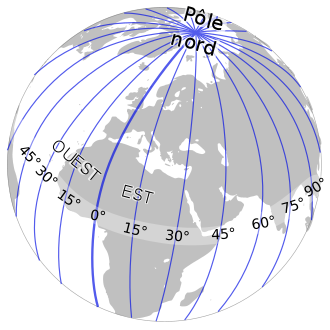
\includegraphics[width=0.3\textwidth]{Images/Cartographie/Longitude.png}
    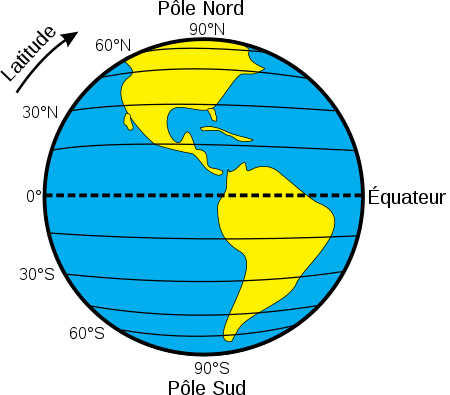
\includegraphics[width=0.3\textwidth]{Images/Cartographie/Latitude.png}
    \caption{Illustration du système de coordonnées de Longitude et Latitude}
    \label{fig:longitude_et_latitude}
\end{figure}

Lorsque l'on combine ce système de coordonnées et une représentation de la Terre en ellipsoïde (au travers de mesures précises des dimensions de la planète), on obtient ce qu'on appelle un système géodésique.

\subsubsection{Le WSG84}

Le World Geodetic System 84 (WGS84) \cite{wgs84} est un système géodésique, et nous pouvons l'utiliser pour nos cartes grâce au paquet "rnaturalearth". Il est notamment utilisé par le système GPS (Global Positioning System). Ce standard a été établi et est maintenu par le National Geospatial Intelligence Agency (NGA) des Etats-Unis \cite{enwiki:1065796786} depuis 1984. Il est basé sur un ellipsoïde de référence raffiné avec le temps pour représenter au mieux la Terre, ainsi que le système de coordonnées en Longitude et Latitude.

Nous avons maintenant un moyen de localiser précisément un point sur Terre grâce à deux valeurs numériques. Pour pouvoir les afficher sur une carte, il nous faut cependant une projection.

\subsubsection{Projections}

La projection cartographique est "un ensemble de techniques permettant de représenter la surface de la Terre dans son ensemble ou en partie sur la surface plane d'une carte" \cite{frwiki:181713838}. La Terre étant (plus ou moins) sphérique, il faut, afin de l'afficher sur une carte plane, la projeter. Il existe différents types de projections, certains permettent de conserver localement les surfaces, d'autres les angles ou encore les distances sur les méridiens. 

Notre paquet utilise de base une projection dite géographique : elle consiste simplement à prendre les valeurs de latitude et de longitude et de les utiliser comme si elles étaient les coordonnées X et Y (respectivement) d'un repère en deux dimensions. Cette "projection" peut avoir des résultats différents en fonction du système géodésique utilisé. 

Le plus gros inconvénient de cette pratique est la distorsion des surfaces lorsque l'on s'éloigne de l'équateur. Cependant, cela est suffisant dans notre cas, où nous voulons avoir seulement une idée globale de la position des lieux observés des uns par rapport aux autres. De plus, comme nous ne prévoyons pas de mesurer précisément la distance entre deux points, ce système de "projection" géographique est le plus pratique.

\subsection{Affichage sur une carte}

Nous connaissons désormais tous les outils pour dessiner nos propres cartes et y placer les lieux de nos observations. Le paquet \emph{rnaturalearth} nous permet d'avoir une liste de polygone de pays et le paquet \emph{ozmaps} nous permet d'avoir les polygones des états australiens. Pour ce qui est des lieux, nous récupérons les latitudes et longitudes manuellement grâce à n'importe quelle base que nous pouvons trouver sur internet et nous les rajoutons à chaque observation en ajoutant deux variables. Finalement nous pouvons afficher notre carte grâce à \emph{ggplot2} et à tous ces différents éléments (voir Figure \ref{fig:carte_australie}).

\begin{figure}[htp]
    \centering
    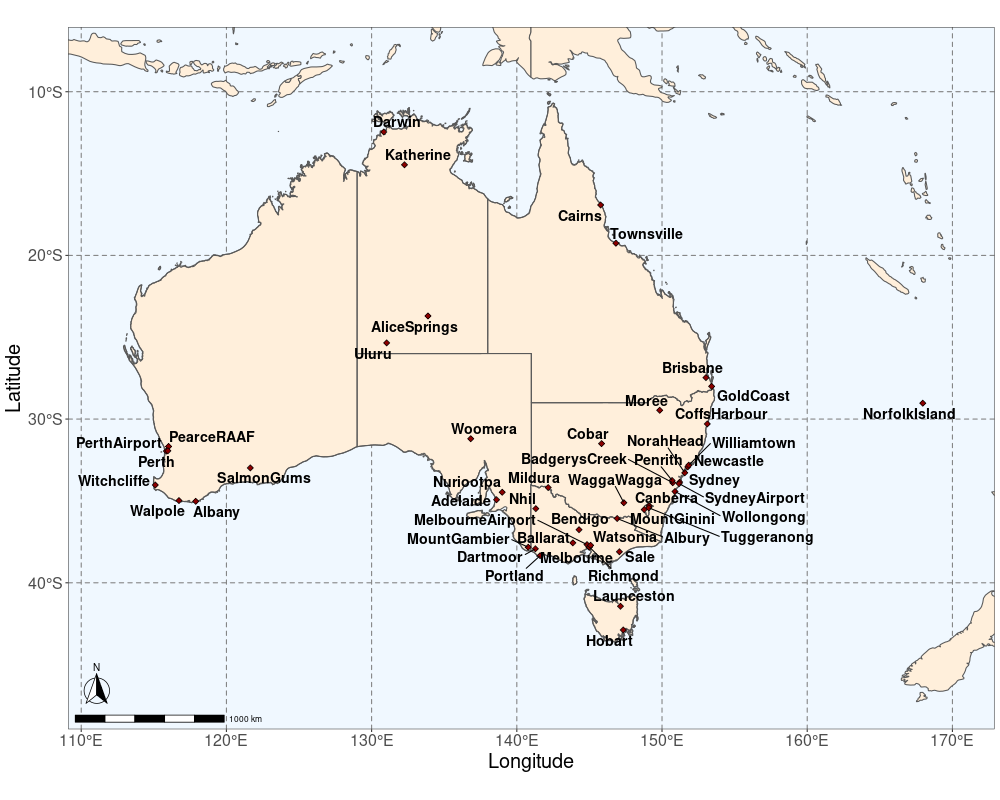
\includegraphics[width=0.7\textwidth]{Images/Cartographie/Australia_full_map.png}
    \caption{Carte de l'Australie avec les lieux observés.}
    \label{fig:carte_australie}
\end{figure}

Nous utilisons désormais les colonnes de longitude et latitude à la place de la colonne localisation. Ainsi, nous nous "débarassons" d'une variable à 49 niveaux pour deux variables numériques.  

\section{Étude des climats}

Maintenant que nous pouvons afficher les lieux sur une carte, nous pouvons déterminer à quelle zone climatique appartient chaque point.

Comme on peut le voir sur la carte précédente, la plupart des observations ont lieu dans le sud-est du pays, où la concentration d'habitants et de ville est la plus grande. Cette zone correspond à un climat tempéré pour les villes les plus au sud et subtropical pour les villes plus au nord comme Brisbane. Au nord du pays nous avons les villes sur les littoraux dans une zone plus tropicale, et enfin au sud-ouest nous avons d'autre villes subtropicales. Plus à l'intérieur des terres, où le climat est désertique, nous avons les observations de Uluru, Alice Springs et Woomera. Enfin, nous avons aussi les données de villes sur l'île de Tasmanie et l'île Norfolk (Figure \ref{fig:carte_climats}) \cite{frwiki:190163125}. 

\begin{figure}[htp]
    \centering
    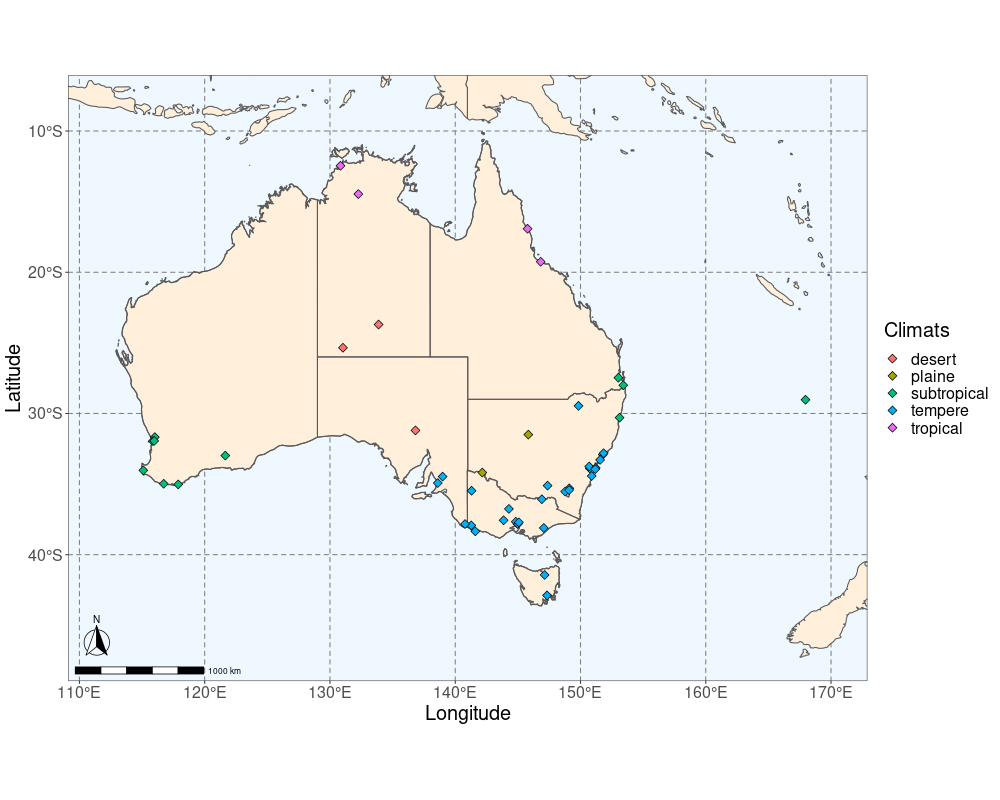
\includegraphics[width=0.9\textwidth]{Images/Cartographie/Australia_climates.png}
    \caption{Carte de l'Australie avec les climats des lieux observés.}
    \label{fig:carte_climats}
\end{figure}

Nous avons donc les observations de 4 lieux tropicaux, 3 lieux désertiques, 2 lieux dans les plaines (le climat de transition entre désertique et tempéré, en quelque sorte), 11 lieux subtropicaux et enfin 29 lieux tempérés. Certaines données sont liées à des villes, mais d'autres à des aéroports ou encore des lieux touristiques.

\subsection{Particularités des climats et périodicité}

Les mesures de météo sont périodiques de périodes de 1 an : on peut mettre en évidence cette périodicité en affichant les moyennes des températures et des précipitations par saison. Nous pourrons ainsi remplacer la variable date par une variable avec uniquement 4 niveaux différents comme expliqué précédemment, à savoir les saisons :
\begin{itemize}
    \item L’été, de décembre à février (niveau 1)
    \item L’automne, de mars à mai (niveau 2)
    \item L’hiver, de juin à août (niveau 3)
    \item Le printemps, de septembre à novembre (niveau 4)
\end{itemize}
Nous obtenons les graphiques de la Figure \ref{fig:temp_and_rainfall}. On remarque tout de suite que les températures les plus élevées sont aux alentours de décembre / janvier ; l'Australie étant dans l'hémisphère sud, il s'agit de l'été. 

\begin{figure}[p]
    \centering
        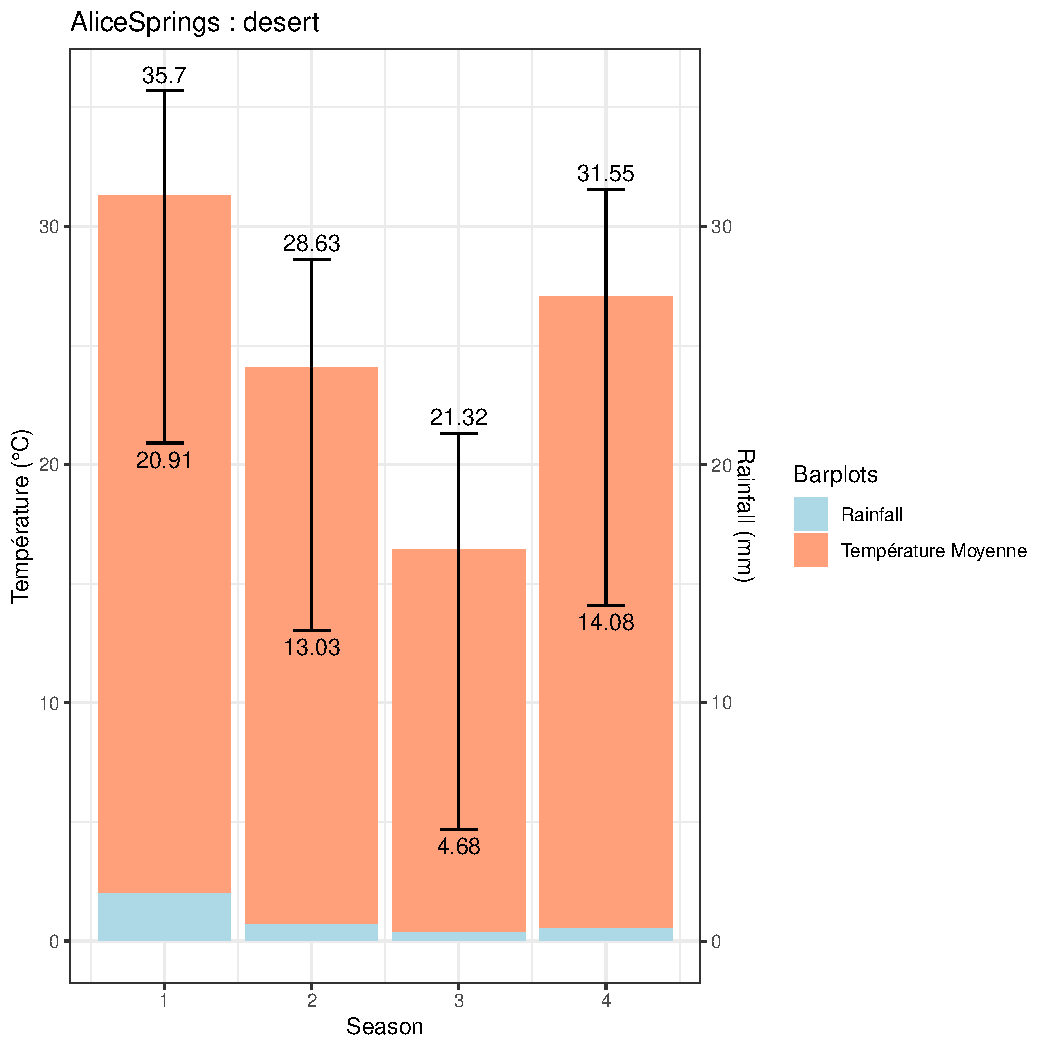
\includegraphics[page=1,width=0.4\textwidth]{Images/temp_and_rainfall/Temp_and_Rainfalldesert.pdf}
        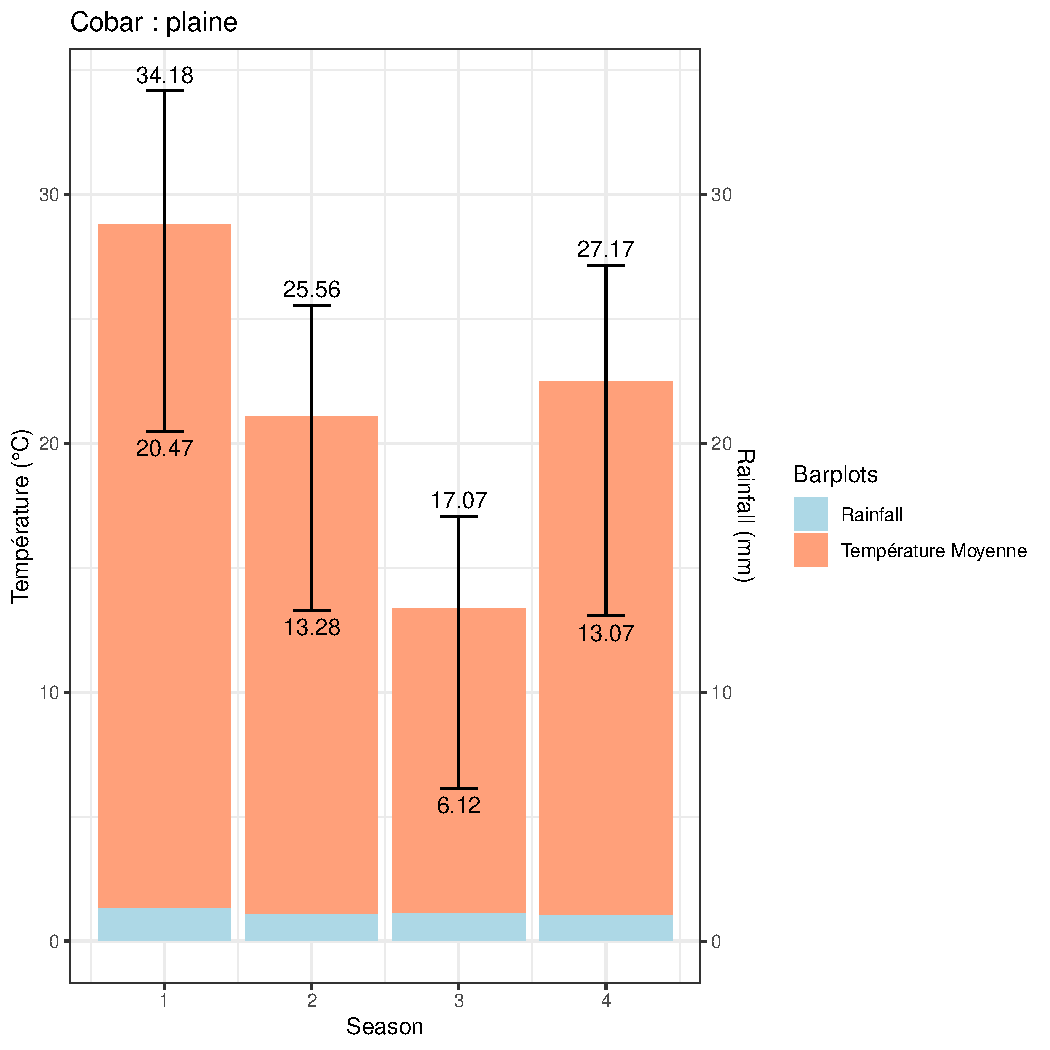
\includegraphics[page=1,width=0.4\textwidth]{Images/temp_and_rainfall/Temp_and_Rainfallplaine.pdf}
        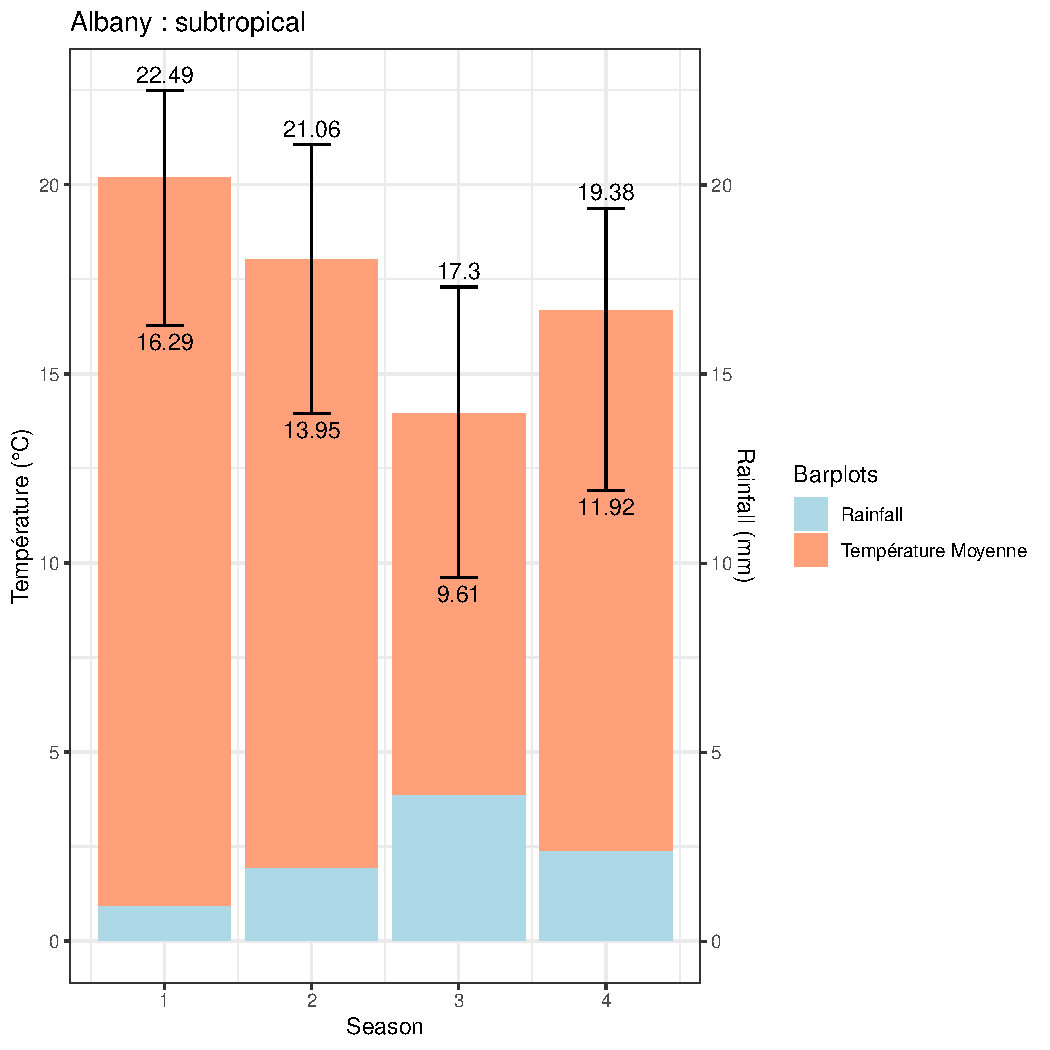
\includegraphics[page=1,width=0.4\textwidth]{Images/temp_and_rainfall/Temp_and_Rainfallsubtropical.pdf}
        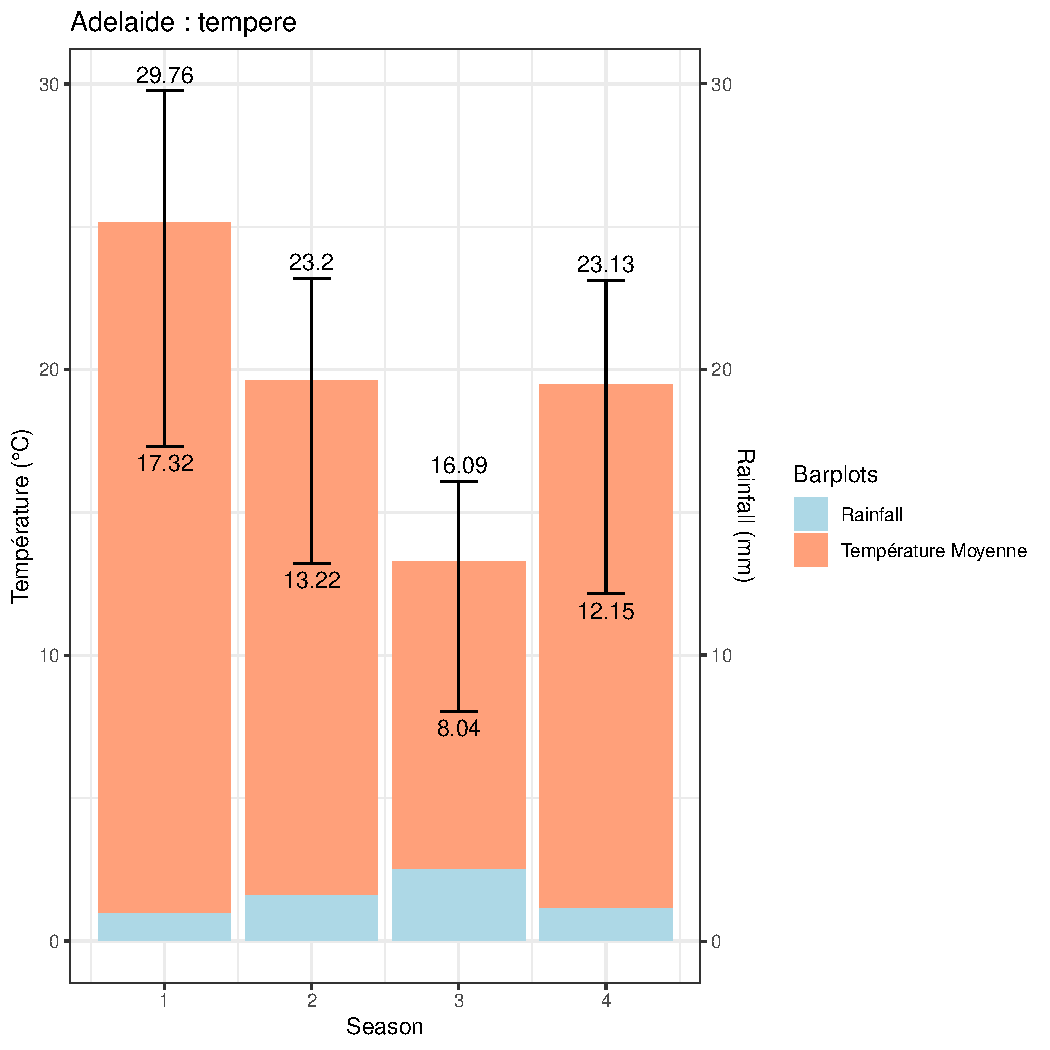
\includegraphics[page=1,width=0.4\textwidth]{Images/temp_and_rainfall/Temp_and_Rainfalltempere.pdf}
        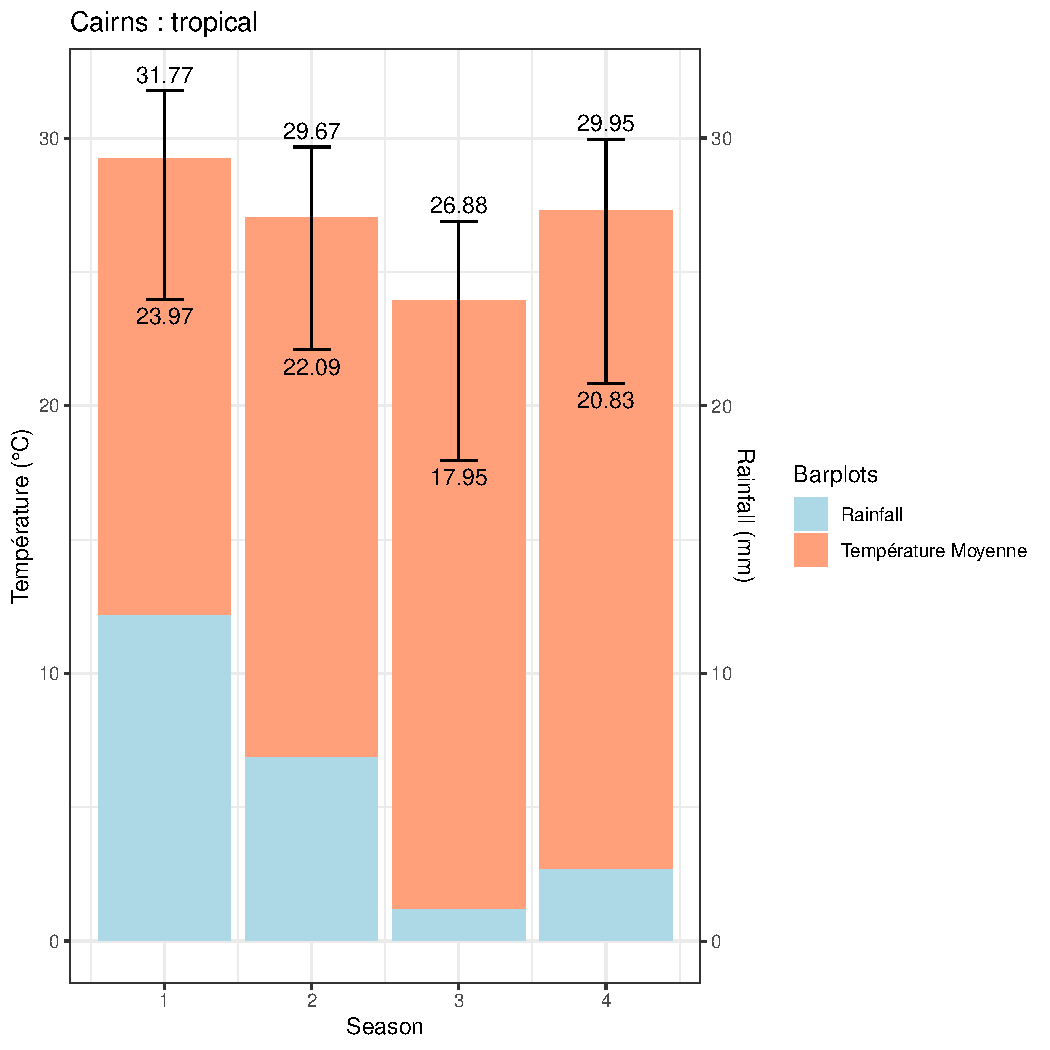
\includegraphics[page=1,width=0.4\textwidth]{Images/temp_and_rainfall/Temp_and_Rainfalltropical.pdf}
    \caption{Température Minimale et Maximale ainsi que pluviométrie au cours d'une année pour certaines des villes des données (une par climat)}
    \label{fig:temp_and_rainfall}
\end{figure}

On remarque ensuite quelques particularités dues aux climats. Dans les régions tempérée et subtropicale tout d'abord, nous avons des températures qui évoluent entre en dessous de 10 degrés et environ 30 degrés, avec en hiver (mai, juin, juillet) plus de pluie que sur le reste de l'année.

Du côté des régions dans les plaines, il pleut moins tout au long de l'année et nous n'observons pas de période de pluie comme pour les deux premières régions. Les températures sont en revanche à peu près les mêmes, voire plus chaudes pendant l'été. Lorsque l'on se penche sur les régions désertiques, les températures sont encore plus hautes et les précipitations sont encore moins importantes, avec seulement quelques millimètres tout au long de l'année. 

À l'opposé, dans les régions tropicales, la température tout au long de l'année évolue moins et reste plus proche de 30 degrés tout au long de l'année (avec une légère baisse en hiver). Dans ces régions, il pleut énormément pendant l'hiver et quasiment pas pendant l'été.

Le choix de ne garder que les saisons et pas les dates se justifie par le fait que si nous voulons prédire s'il pleut le lendemain, nous n'avons pas besoin de savoir précisément quel jour nous sommes, voire quel mois. On remarque sur les graphiques des différences notables entre les saisons, et celle-ci suffiront sûrement pour nous aider à prédire ce que nous voulons. De plus, nous nous débarrassons d'une variable avec beaucoup de facteurs différents, ce qui nous sera bénéfique lors de la mise en place de modèle de prédictions.

Nous nous retrouvons finalement avec les variables suivantes : 
\begin{itemize}
    \item MinTemp, MaxTemp, Temp9am, Temp3pm
    \item Rainfall, RainToday, RainTomorrow, Evaporation
    \item Sunshine, Cloud9am, Cloud3pm
    \item WindGustDir, WindGustSpeed, WindDir9am, WindDir3pm, WindSpeed9am, WindSpeed3pm
    \item Humidity9am, Humidity3pm
    \item Pressure9am, Pressure3pm
    \item Season, Climate
    \item Latitude, Longitude
\end{itemize}
Qui sont toutes des variables numériques, sauf pour Season et Climate qui sont à 4 et 5 niveaux, et RainToday et RainTomorrow qui sont des variables booléennes.

\section{Complétion des données}

\subsection{Pourquoi compléter ?}

Afin de se rendre compte de la distribution des valeurs manquantes, on affiche ce qu'on appelle la \emph{missingness map} de nos données (Figure \ref{fig:missingness_raw}).

\begin{figure}[htp]
    \centering
    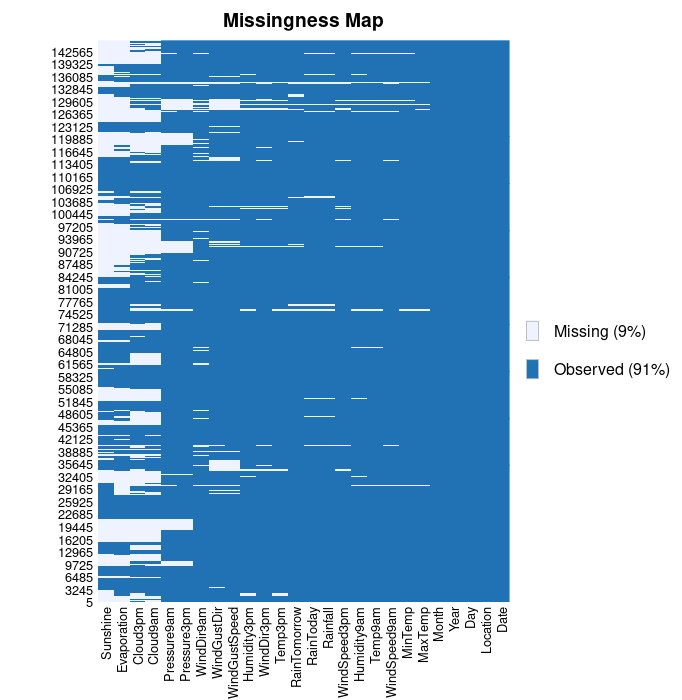
\includegraphics[width=0.5\textwidth]{Images/missmap.png}
    \caption{Missingness Map des données avant la complétion.}
    \label{fig:missingness_raw}
\end{figure}

Pour pouvoir faire des prédictions sur nos données, nous avons besoin de nous débarrasser des observations avec des valeurs \emph{NA}. Pour cela, on utilise la commande \mintinline{R}{na.omit}. On se retrouve avec $56420$ observations sur les $145460$ de base, ce qui est très peu. De plus, la plupart des lieux ne sont plus représentés comme nous l'indique la Figure \ref{fig:distrib_raw}.

\begin{figure}[htp]
    \centering
    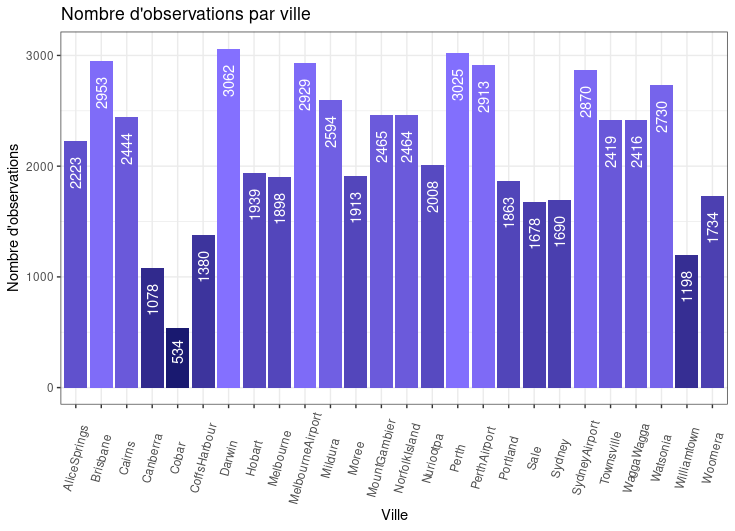
\includegraphics[width=0.7\textwidth]{Images/distribution_lieux_raw.png}
    \caption{Distribution du nombre d'observations après un \emph{na.omit}.}
    \label{fig:distrib_raw}
\end{figure}

Nous allons donc chercher un moyen de compléter les valeurs \emph{NA}, et de le faire de façon à ne pas avoir trop de données redondantes et de garder une cohérence vis-à-vis des climats des lieux observés.

\subsection{Comment compléter ?}

Pour compléter nos données, nous allons regarder pour chaque variable quels sont les lieux qui ont besoin de complétion ; disons ceux qui ont plus de 20\% de \emph{NA} pour cette variable, et quels sont ceux avec lesquels nous pouvons compléter : les autres qui ont plus de 2500 observations et qui ont au moins 80\% de leurs observations complètes. Nous excluons ainsi les lieux dont nous n'avons pas les observations sur les dix ans : lorsque nous complétons nos données, nous voulons que les dates coïncident pour ne pas perdre en cohérence, ainsi nous voulons compléter les données avec les lieux pour lesquels nous avons des observations sur la période maximale d'observation de notre base de données, soit plus de 2500 jours. Le seuil de 80\% des données est choisi pour avoir un maximum d'observations sans \emph{NA} et pour être sûr d'avoir une ville depuis laquelle copier les données.

Lorsque nous copions les données d'un lieu à un autre, nous nous soucions donc de la date d'observation. Cependant, cela ne suffira pas. Nous avons vu en effet que les différents lieux observés appartiennent à des zones climatiques très différentes. Pour chaque variable, nous allons donc associer nos deux listes de lieux (ceux à compléter et ceux avec lesquels compléter) en cherchant les lieux les plus proches géographiquement de la même zone climatique. 

Finalement, nous nous retrouvons avec une liste de couples pour chaque variable.

Avec cette méthode, nous allons copier jusqu'à 5 fois maximum les données d'un lieu pour un autre lieu, et nous le ferons de manière "intelligente", sans perte de cohérence par rapport aux climats des lieux observés. Nous pouvons afficher quelles données de quelles villes vont compléter quelles autres villes sur des cartes, cf. les Figures \ref{fig:path_data1} à \ref{fig:path_data4} de l'Annexe. On peut voir que pour les variables où il y avait le plus de \emph{NA}, beaucoup de lieux sont complétés. Dans d'autre cas moins extrêmes, nous n'avons copié les données que d'un seul lieu à un seul autre. 


\subsection{Après complétion}

Finalement, le \emph{na.omit} nous donne une base de données avec $105546$ observations. On peut réafficher la \emph{missingness map} et la distribution des observations par lieu (respectivement Figures \ref{fig:missingness_completed} et \ref{fig:distrib_completed})

\begin{figure}[htp]
    \centering
    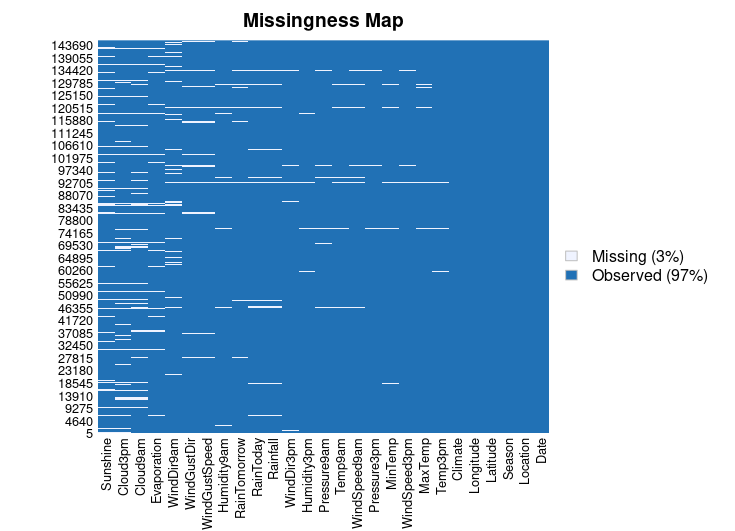
\includegraphics[width=0.5\textwidth]{Images/missmap_completed.png}
    \caption{Missingness Map des données complétées.}
    \label{fig:missingness_completed}
\end{figure}

\begin{figure}[htp]
    \centering
    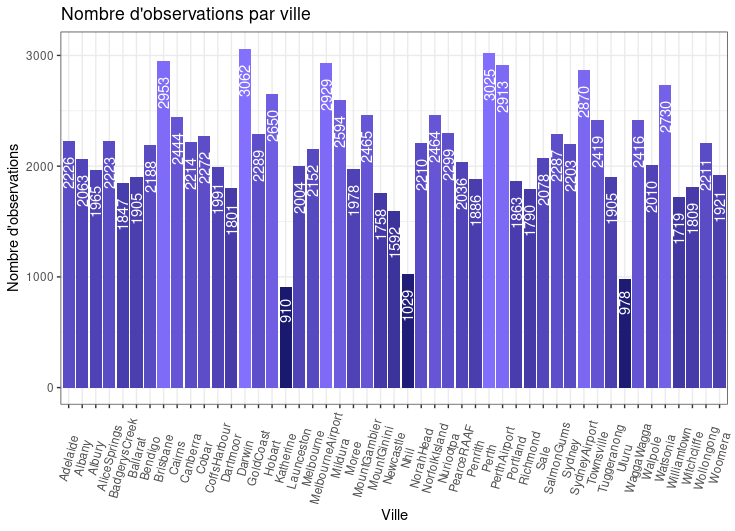
\includegraphics[width=0.6\textwidth]{Images/distribution_lieux_completed.png}
    \caption{Distribution des observations par villes dans notre base de données finale.}
    \label{fig:distrib_completed}
\end{figure}

On remarque que certaines plages de dates n'ont pas été complétées pour certaines variables, il peut y avoir deux raisons à cela : 
\begin{itemize}
    \item Le lieu pour cette variable n'a pas été considéré comme "à compléter", malgré quelques valeurs \emph{NA};
    \item Le lieu qui a servi pour la complétion certaines dates en moins que celles du lieu à compléter.
\end{itemize}
Le nombre d'observations de notre base de données finale reste cependant satisfaisant et tous les lieux sont représentés.

\section{Relations entre les variables}

Dans cette partie nous allons chercher à mettre en lumière les relations entre les variables.

\subsection{Corrélations entre les variables numériques}

Commençons tout d'abord par nous renseigner sur les corrélations entre les variables numériques (Figure \ref{fig:correlations}). 

\begin{figure}[htp]
    \centering
    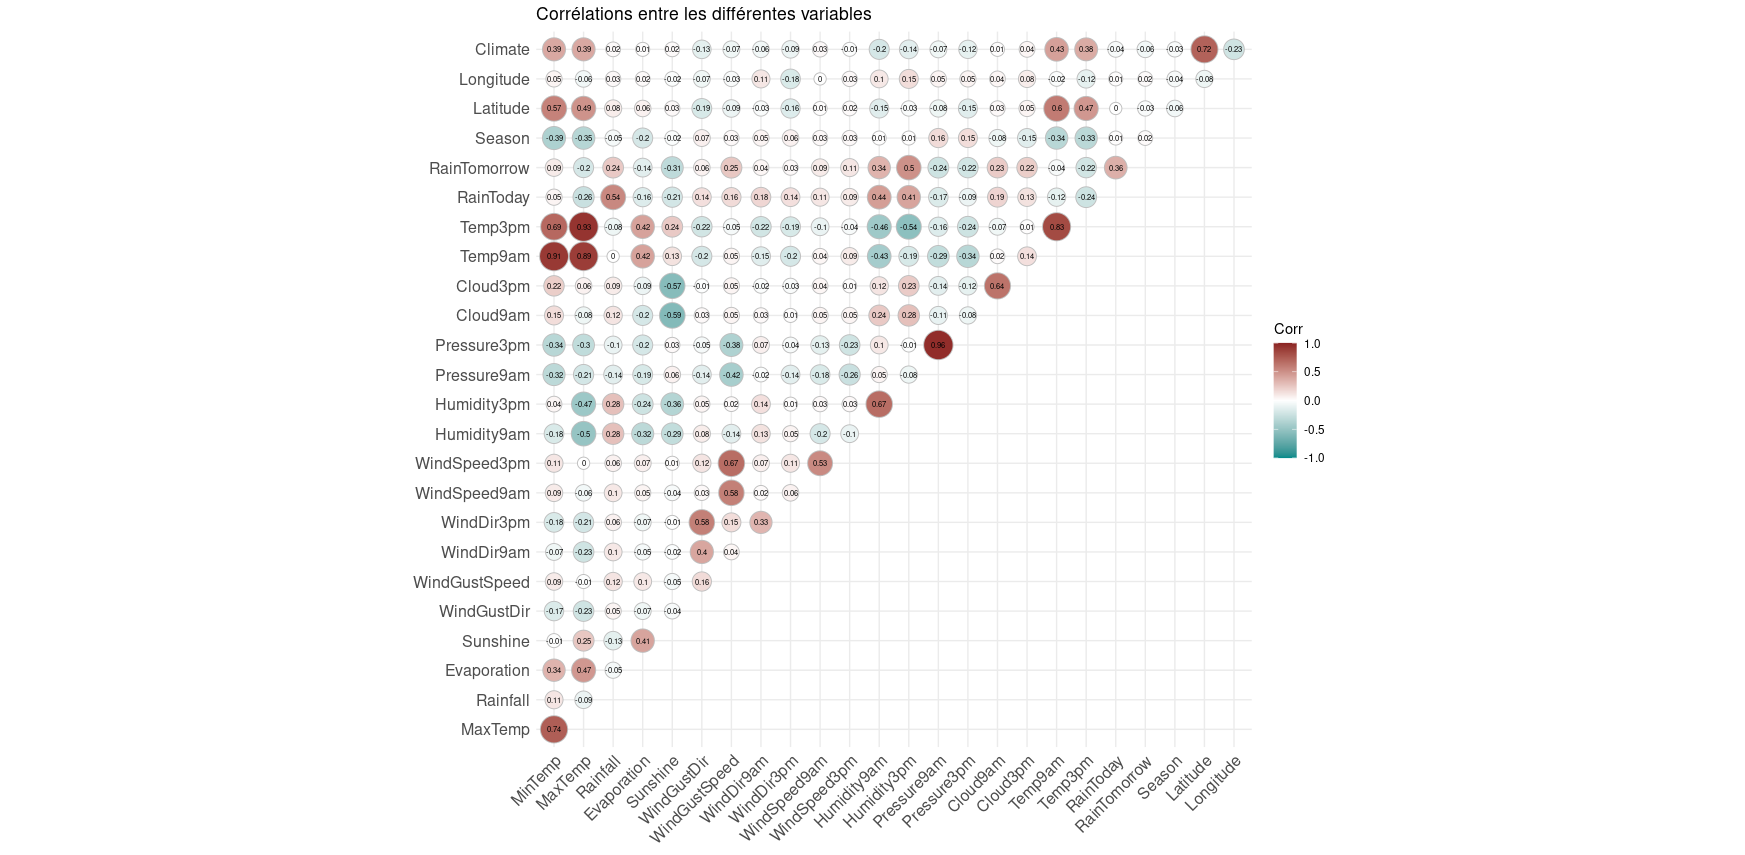
\includegraphics[width=\textwidth]{Images/correlations_variables.png}
    \caption{Corrélations des variables deux-à-deux.}
    \label{fig:correlations}
\end{figure}

Nous pouvons conclure de cette figure les points suivants : 
\begin{itemize}
    \item Concernant les variables de températures : 
    \begin{itemize}
        \item MinTemp et MaxTemp sont deux variables corrélées (coeff. = 0.73). C'est un résultat attendu, car ces deux valeurs sont les températures maximales et minimales de la même journée. 
        \item Temp9am et Temp3pm sont fortement corrélées (coeff. = 0.83). Ce résultat était attendu pour la même raison qui explique la corrélation entre MinTemp et MaxTemp.
        \item MinTemp et Temp9am sont très corrélées (coeff. = 0.9). La température minimale d'une journée est atteinte aux alentours de 9h du matin, il est normal d'avoir ce résultat. 
        \item MaxTemp et Temp3pm sont très corrélées (coeff. = 0.94). La température maximale d'une journée est atteinte aux alentours de 15h, ce résultat était donc attendu. 
        \item Nous pouvons aussi remarquer que le couple Temp3pm et MinTemp et le couple Temp9am et MaxTemp sont aussi corrélés (coeff. resp. = 0.69 et 0.89). La température maximale est cependant plus corrélées à celle à 9h du matin que ne l'est la température minimale et la température à 15h. Cela peut s'expliquer par le fait qu'en fonction des saisons, le soleil se lève plus ou moins tôt, et que donc à 9h déjà, il peut faire très chaud. Dans tous les cas, il est normal que ces températures soient corrélées puisqu'il s'agit des écarts de températures d'une même journée. Ces derniers ne sont pas très importants et dépendent énormément de la saison (donc de la journée) comme nous l'avons vu Figure \ref{fig:temp_and_rainfall}. 
    \end{itemize}
    \item La variable Latitude est corrélée positivement aux variables de températures (la température dépend des climats et ces climats sont très dépendants de la latitude comme on a pu le voir dans la partie cartographie).
    \item Pression9am et Pression3pm sont très corrélées (coeff. = 0.96) pour les mêmes raisons que les variables de température. Il en va de même pour Humidity3pm et Humidity9am (coeff = 0.66) et WindSpeed3pm et WindSpeed9am (0.49).
    \item WindSpeed3pm est corrélée positivement avec WindGustDir (coeff. = 0.66).
    \item Les variables Cloud9am et Cloud3pm sont corrélées négativement avec la variable Sunshine (-0.57 et -0.55 respectivement) ce qui est logique, car ils mesurent à peu près la même chose. 
    \item Les variables d'humidité sont corrélées négativement à MaxTemp (-0.48 et -0.5).
\end{itemize}

\subsection{Boîtes à moustaches pour les variables à facteurs}

Affichons maintenant les Boîtes à moustaches des valeurs des différentes variables continues en fonction de nos variables à facteurs. 

\begin{figure}[htp]
    \centering
    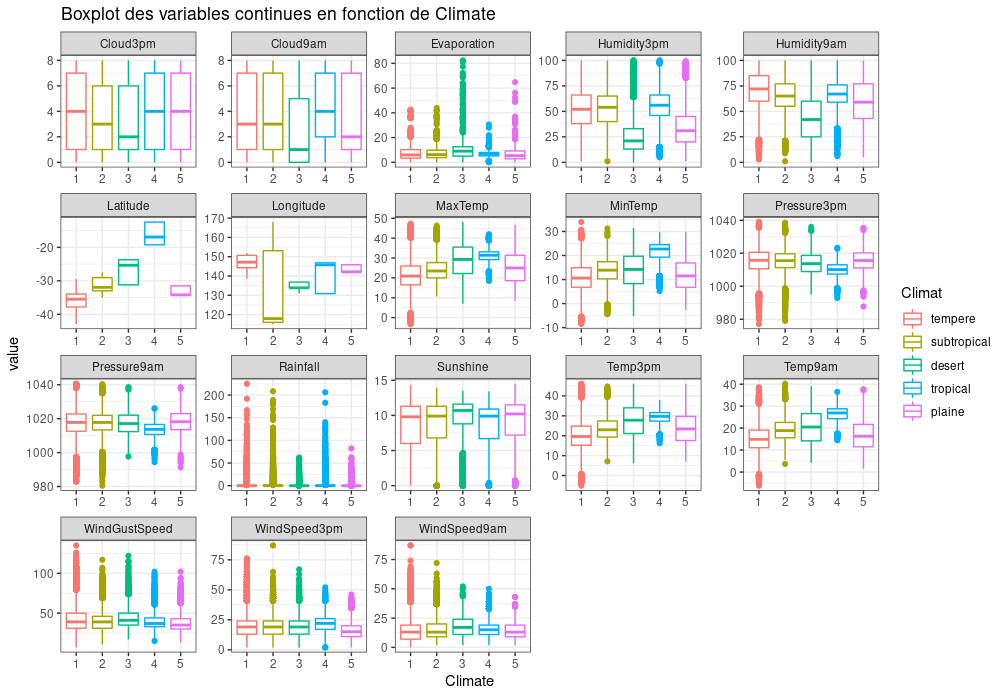
\includegraphics[width=0.8\textwidth]{Images/boxplots/boxplot_Climate.png}
    \caption{Boîtes à moustaches pour la variable Climate}
    \label{fig:bp_climate}
\end{figure}

Pour la variable Climate (Figure \ref{fig:bp_climate}), on voit une fois de plus la différence entre les climats de désert et de plaine et les autres au niveau de leur humidité. Cela se voit aussi avec le nombre de grandes valeurs de Rainfall (en dehors des moustaches). On peut aussi voir que les climats sont arrangés en couche du nord au sud de l'Australie, comme on pouvait voir sur la carte plus haut. En effet, la région tropicale est au nord du pays, comme l'indique la boîte à moustache concernant la Latitude. Tout au sud on trouve la région tempérée. On peut aussi trouver une différence de températures entre ces 5 climats, avec une distribution ressemblant à celle de la Latitude : la région tropicale est la plus chaude et la moins chaude est la région tempérée. 

\begin{figure}[htp]
    \centering
    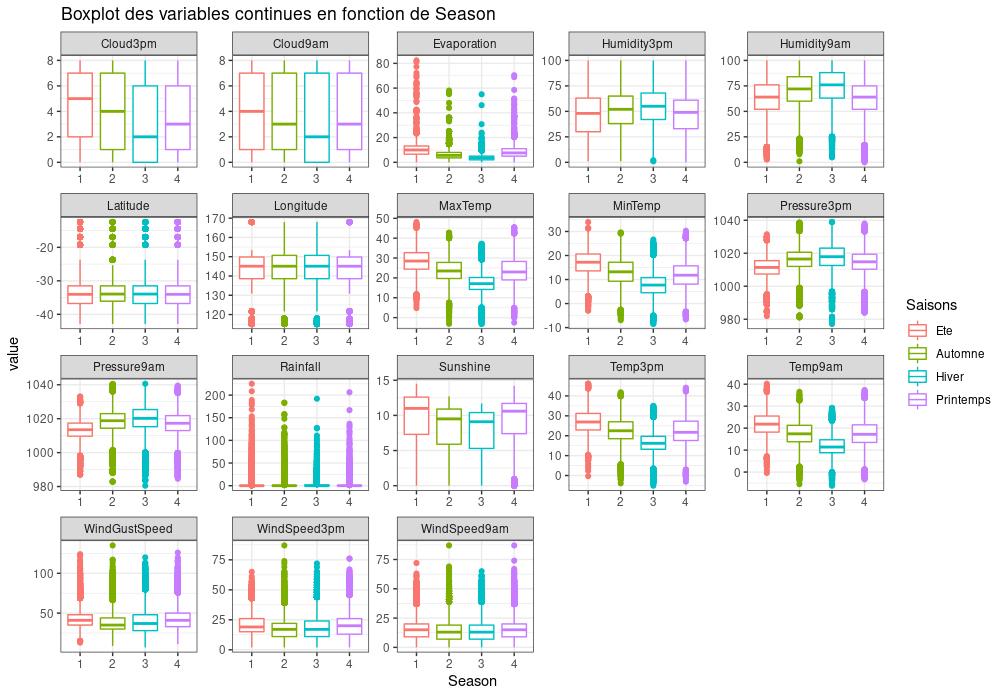
\includegraphics[width=0.8\textwidth]{Images/boxplots/boxplot_Season.png}
    \caption{Boîtes à moustaches pour la variable Season}
    \label{fig:bp_season}
\end{figure}

Penchons-nous désormais sur les boîtes à moustaches de la variable Season (Figure \ref{fig:bp_season}). On trouve la distribution des températures auxquelles nous nous attendions : il fait plus chaud en été et moins en hiver. Ce même schéma est visible pour le taux d'ensoleillement (et donc un peu pour les variables des nuages). Les variables de pression et d'humidité évolues similairement : elles augmentent en hiver. En effet, la pression peut changer en fonction des dépressions (qui apportent souvent le mauvais temps) ou la vitesse du vent \cite{frwiki:190112465}.

\begin{figure}[htp]
    \centering
    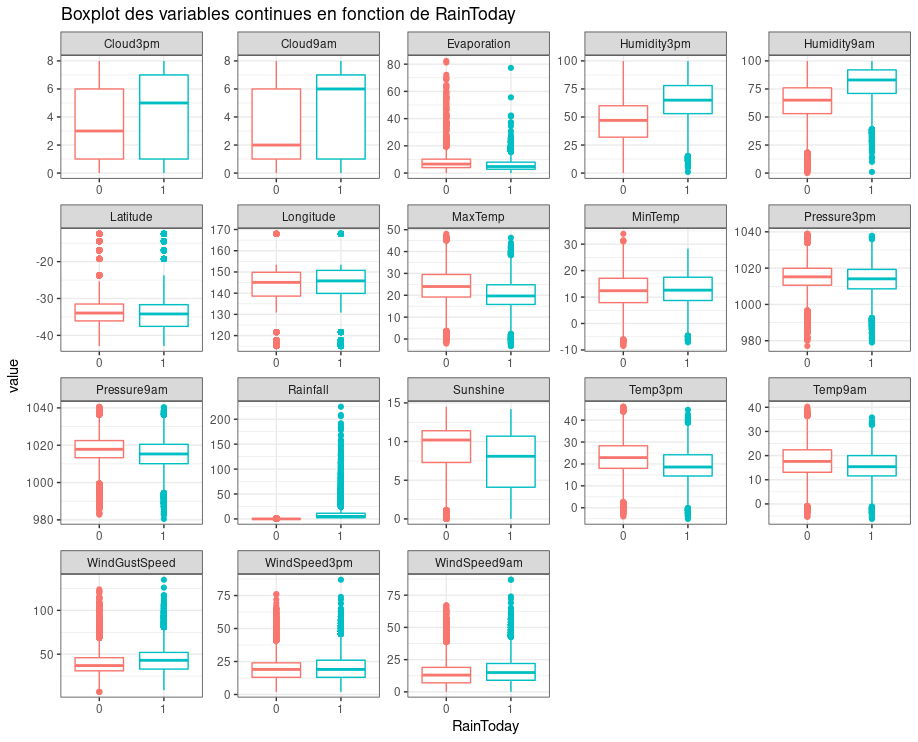
\includegraphics[width=0.7\textwidth]{Images/boxplots/boxplot_RainToday.png}
    \caption{Boîtes à moustaches pour la variable RainToday}
    \label{fig:bp_raintoday}
\end{figure}

\begin{figure}[htp]
    \centering
    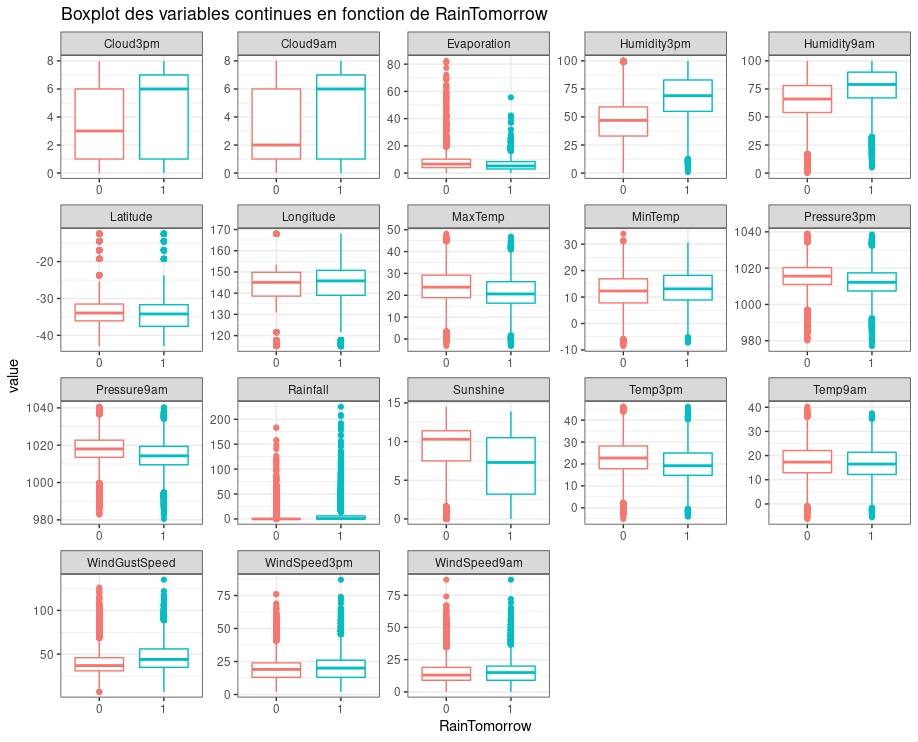
\includegraphics[width=0.7\textwidth]{Images/boxplots/boxplot_RainTomorrow.png}
    \caption{Boîtes à moustaches pour la variable RainTomorrow}
    \label{fig:bp_raintomorrow}
\end{figure}

Jetons maintenant un coup d'œil aux boîtes des variables RainToday (Figure \ref{fig:bp_raintoday}) et RainTomorrow (Figure \ref{fig:bp_raintomorrow}). Comme on peut s'y attendre elles sont très similaires. En effet, d'un jour au lendemain, il n'y a pas de changement énorme. Comme ces deux variables sont liées (si RainToday alors RainTomorrow pour le jour d'avant), nous avons ces similarités. Une différence notable est celle des boîtes affichées pour la variable Rainfall : par construction de la variable RainToday, il n'y a pas d'observations ou Rainfall a une valeur supérieure à 0 et ou RainToday est à 1. Ça n'est pas le cas pour RainTomorrow évidemment, il y aura toujours un moment ou il pleut aujourd'hui mais il ne pleuvra pas demain (sinon la pluie ne s'arrêterait jamais).

Comme on peut s'y attendre, les variables d'humidité sont plus élevées lorsqu'il pleut (RainToday). On peut voir cependant ces mêmes différences pour RainTomorrow, avec quelques variations : l'humidité à 15h et à 9h est plus élevée lorsqu'il pleut le lendemain (cette différence est surtout notable pour Humidity3pm, les distances interquartiles ne se chevauchent presque pas). Cette variable est peut-être une des plus importantes dans la prévision de RainTomorrow.

\newpage
\part{Prédiction}

Maintenant que notre base de données est prête que nous la connaissons plus en détail, nous pouvons commencer à créer nos modèles de prédiction. Commençons tout d'abord par faire une analyse en composantes principales, pour avoir une meilleure idée de la distribution des observations.

\section{ACP et déséquilibre}

Rappelons tout d'abord la distribution des observations où il pleut le lendemain et où il ne pleut pas : 

\begin{table}[H]
    \centering
        \begin{tabular}{|rrr|}
            \hline
            RainTomorrow & Compte & \% \\ 
            \hline
            \hline
            0 & 82367 & 78.04 \\
            1 & 23179 & 21.96 \\
            \hline
        \end{tabular}
    \caption{Distribution des valeurs de RainTomorrow.}
\end{table}

Et lorsque l'on affiche une analyse en composantes principales de ces observations, et en les colorant en fonction de leur valeur de RainTomorrow, on obtient le graphique de la Figure \ref{fig:pca_raintomorrow}.

\begin{figure}[htp]
    \centering
    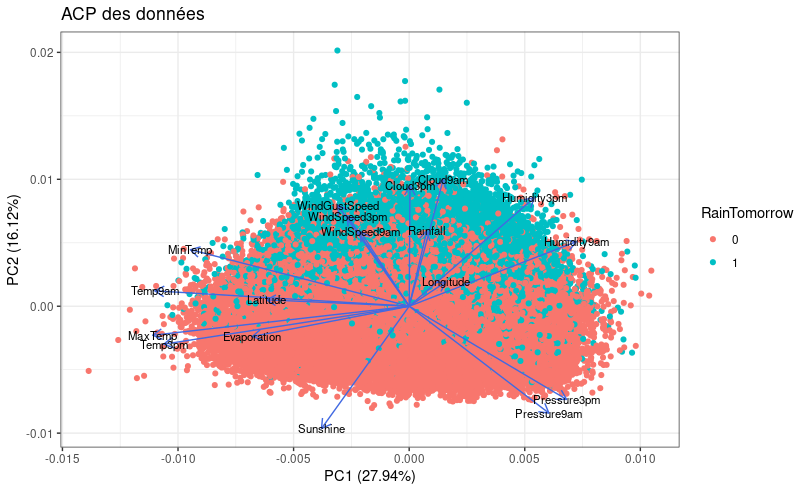
\includegraphics[width=0.8\textwidth]{Images/pca/pca.png}
    \caption{Analyse en Composantes Principales de nos données, points colorés en fonction de RainTomorrow.}
    \label{fig:pca_raintomorrow}
\end{figure}

Nous allons donc chercher un moyen de séparer ces deux groupes pour faire des prédictions. On voit déjà (avec 44.06\% de l'information, l'axe 1 représentant 27.94\% et l'axe 2 16.12\%) que les observations pour lesquelles il pleut le lendemain sont un peu séparées de celles où il ne pleut pas. On voit d'ailleurs bien le déséquilibre de nos données sur ce graphique.

On peut noter par ailleurs que les variables d'humidité et des nuages sont importantes pour différencier ces deux groupes. En effet, les valeurs de ces variables sont plus élevées pour RainTomorrow = 1. À l'inverse, lorsque la valeur de Sunshine est élevée, on va plutôt vers le groupe RainTomorrow = 0. On peut aussi s'amuser à regarder les 2 composantes principales suivantes pour avoir un autre point de vue (on a cette fois-ci 28.51\% de l'information, Figure \ref{fig:pca_raintomorrow2}).

\begin{figure}[htp]
    \centering
    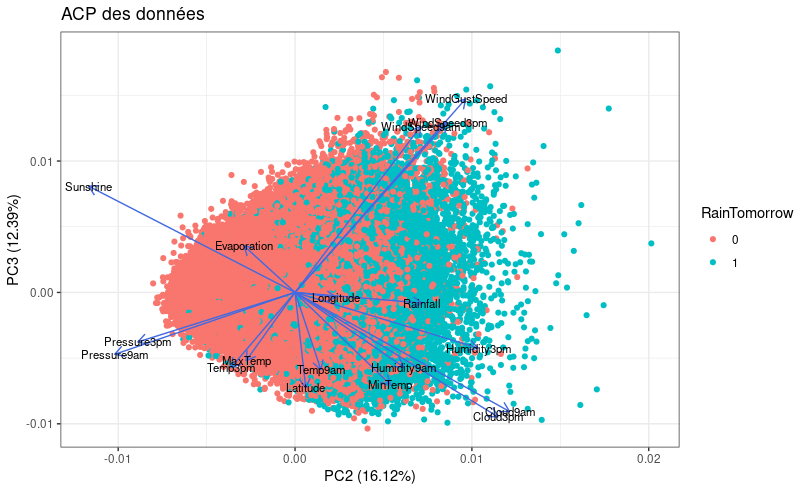
\includegraphics[width=0.8\textwidth]{Images/pca/pca2.png}
    \caption{Analyse en Composantes Principales de nos données, axes 2 et 3, points colorés en fonction de RainTomorrow.}
    \label{fig:pca_raintomorrow2}
\end{figure}

Il semble aussi que les variables de pression sont importantes pour différencier ces deux groupes. 

\section{Premières prédictions}

Dans cette partie nous allons prendre telle quelle la base de données, sans nous soucier de son déséquilibre. Nous allons mettre en place un modèle de régression linéaire logistique.

Évidemment, nous séparerons nos données en deux échantillons : un échantillon d'apprentissage (dataApp), correspondant à 80\% des données choisies de manière aléatoire et un échantillon pour les tests (dataTest) correspondant aux 20\% restants.

Nous allons construire ce modèle sur différentes "versions" de notre base de données : équilibrée ou non, avec du \emph{one-hot encoding} ou non (à chaque fois séparés en dataApp et dataTest), afin de mettre en évidence l'utilité de ces étapes supplémentaires.

\subsection{Le \emph{one-hot encoding}}

Lorsque nous avons une variable à plusieurs niveaux, dans notre cas les variables Climate et Season, nous pouvons les transformer pour nous servir de l'information qu'elles nous procurent avec des variables numériques. 

Pour chaque niveau de la variable, nous allons créer une variable. Ainsi, comme nous avons 4 saisons, nous aurons 4 nouvelles variables : Season.1, Season.2, Season.3 et Season.4. Comme nous avons déjà fait un travail pour réduire le nombre de niveaux pour les variables avec des facteurs, nous n'aurons pas beaucoup plus de colonnes dans notre base de données. 

Pour remplir ces nouvelles variables, nous allons mettre un "1" dans la colonne qui correspond au niveau de la saison de la mesure et "0" dans les autres. Imaginons en effet qu'une observation a eu lieu en automne (c'est-à-dire que sa valeur pour la variable Season est 2), alors les 4 colonnes seront remplies de la façon suivante : 

\begin{table}[H]
    \centering
    \begin{tabular}{|rrrr|}
        \hline
        Season.1 & Season.2 & Season.3 & Season.4 \\
        \hline 
        0 & 1 & 0 & 0 \\
        \hline
    \end{tabular}
    \caption{\emph{one-hot encoding} de la variable Season sur une observation d'automne}
\end{table}

Nous faisons de même avec Climate. Ainsi nous passons de 2 colonnes à 9 : 

\begin{table}[ht]
    \centering
    \resizebox{\textwidth}{!}{
        \begin{tabular}{|rrrrrrrrr|}
            \hline
            Season.1 & Season.2 & Season.3 & Season.4 & Climate.1 & Climate.2 & Climate.3 & Climate.4 & Climate.5 \\ 
            \hline
            1.00 & 0.00 & 0.00 & 0.00 & 1.00 & 0.00 & 0.00 & 0.00 & 0.00 \\ 
            1.00 & 0.00 & 0.00 & 0.00 & 1.00 & 0.00 & 0.00 & 0.00 & 0.00 \\ 
            1.00 & 0.00 & 0.00 & 0.00 & 1.00 & 0.00 & 0.00 & 0.00 & 0.00 \\ 
            1.00 & 0.00 & 0.00 & 0.00 & 1.00 & 0.00 & 0.00 & 0.00 & 0.00 \\ 
            1.00 & 0.00 & 0.00 & 0.00 & 1.00 & 0.00 & 0.00 & 0.00 & 0.00 \\ 
            1.00 & 0.00 & 0.00 & 0.00 & 1.00 & 0.00 & 0.00 & 0.00 & 0.00 \\ 
            \hline
        \end{tabular}
    }
    \caption{Extrait du début des variables après \emph{one-hot encoding} des variables Season et Climate.}
\end{table}

Nous voilà maintenant avec une base de données ne contenant que des variables numériques et une variable (RainTomorrow) de facteurs. Nous pouvons utiliser des techniques d'\emph{up-sampling} comme le SMOTE (nous rentrerons dans les détails plus tard).

\subsection{Une première régression linéaire logistique}

Construirons donc notre modèle de régression logistique. Pour cela, nous allons utiliser la fonction \emph{glm} de la librairie \emph{stats} de R. En utilisant le paramètre "family = binomial", nous pouvons faire une régression logistique, qui prend en compte les variables factorielles. Nous ne faisons donc pas encore de \emph{one-hot encoding} et gardons la base de données telle quelle. 

Un \emph{summary} de ce modèle nous montre : 
\begin{minted}{R}
    Call:
    glm(formula = RainTomorrow ~ ., family = binomial, data = dataApp)
    
    Deviance Residuals: 
        Min       1Q   Median       3Q      Max  
    -3.0799  -0.5630  -0.3302  -0.1500   3.2469  
    
    Coefficients:
                    Estimate Std. Error z value Pr(>|z|)    
    (Intercept)    4.538e+01  1.790e+00  25.349  < 2e-16 ***
    MinTemp        1.567e-02  5.504e-03   2.847  0.00442 ** 
    MaxTemp       -6.312e-02  5.926e-03 -10.652  < 2e-16 ***
    Rainfall       1.668e-02  1.584e-03  10.526  < 2e-16 ***
    Evaporation    2.418e-04  3.100e-03   0.078  0.93783    
    Sunshine      -6.412e-02  3.735e-03 -17.168  < 2e-16 ***
    WindGustDir    1.754e-04  1.318e-04   1.331  0.18333    
    WindGustSpeed  5.620e-02  1.162e-03  48.359  < 2e-16 ***
    WindDir9am    -3.727e-04  1.190e-04  -3.132  0.00174 ** 
    WindDir3pm    -7.989e-05  1.329e-04  -0.601  0.54767    
    WindSpeed9am  -1.354e-02  1.573e-03  -8.604  < 2e-16 ***
    WindSpeed3pm  -3.047e-02  1.639e-03 -18.597  < 2e-16 ***
    Humidity9am    9.532e-03  1.077e-03   8.852  < 2e-16 ***
    Humidity3pm    5.313e-02  1.023e-03  51.915  < 2e-16 ***
    Pressure9am    1.019e-01  5.925e-03  17.192  < 2e-16 ***
    Pressure3pm   -1.517e-01  5.860e-03 -25.893  < 2e-16 ***
    Cloud9am       2.585e-03  4.836e-03   0.534  0.59301    
    Cloud3pm       4.043e-02  5.098e-03   7.931 2.17e-15 ***
    Temp9am        5.863e-02  8.532e-03   6.872 6.31e-12 ***
    Temp3pm        3.384e-02  4.235e-03   7.989 1.36e-15 ***
    RainToday1     5.710e-01  2.791e-02  20.457  < 2e-16 ***
    Season2        3.692e-01  3.288e-02  11.226  < 2e-16 ***
    Season3        6.623e-01  4.272e-02  15.505  < 2e-16 ***
    Season4        4.318e-01  3.324e-02  12.992  < 2e-16 ***
    Latitude       6.860e-03  4.780e-03   1.435  0.15121    
    Longitude     -1.338e-02  1.096e-03 -12.205  < 2e-16 ***
    Climate2      -1.288e-01  3.931e-02  -3.276  0.00105 ** 
    Climate3      -3.819e-01  8.957e-02  -4.264 2.01e-05 ***
    Climate4      -1.001e+00  1.026e-01  -9.757  < 2e-16 ***
    Climate5       1.398e-01  6.631e-02   2.108  0.03502 *  
    ---
    Signif. codes:  0 ‘***’ 0.001 ‘**’ 0.01 ‘*’ 0.05 ‘.’ 0.1 ‘ ’ 1
    
    (Dispersion parameter for binomial family taken to be 1)
    
        Null deviance: 88900  on 84437  degrees of freedom
    Residual deviance: 61568  on 84408  degrees of freedom
    AIC: 61628
    
    Number of Fisher Scoring iterations: 5
\end{minted}

On remarque que la fonction a fait elle-même le \emph{one-hot encoding}, et on retrouve des variables supplémentaires pour les différents niveaux des variables à niveaux. On remarque cependant qu'il y en a à chaque fois une de moins que le nombre de niveaux : en fait, cela suffit à donner l'information du dernier niveau si dans tous ceux déjà présent nous avons "0". En effet, si pour une observation nous avons les variables Climate "2" à "5" égales à "0", alors nous savons que cette observation est dans une région climatique "1". 

Chose intéressante : si d'ailleurs on relançait cette fonction avec nos données après le \emph{one-hot encoding} que nous avons spécifié plus haut, nous verrons devant chacune des colonnes "redondantes" un coefficient égal à \emph{NA} (la variable est ignorée car colinéaire aux autres).

La première chose que nous pouvons remarquer de cette sortie R est que nous avons des coefficients qui ne peuvent pas être jugés comme significativement non nuls. En effet, pour les variables Evaporation, WindGustDir, WindDir3pm, Cloud9am et Latitude, la p-value du test de Student est bien supérieure à 0.05. Nous pouvons donc mettre en œuvre une sélection pas-à-pas de ces régresseurs.  

La fonction \emph{confusionMatrix} de la librairie \emph{caret} nous permet de voir rapidement les performances de notre modèle. Sur dataApp (à gauche) et dataTest (à droite) : 

\begin{multicols}{2}
    \begin{minted}{text}
    Confusion Matrix and Statistics

        y.app
    y.glm     0     1
        0 62377  9722
        1  3517  8822
                                            
                 Accuracy : 0.8432          
                   95% CI : (0.8407, 0.8457)
      No Information Rate : 0.7804          
      P-Value [Acc > NIR] : < 2.2e-16       
                                           
                    Kappa : 0.4801          
                                          
   Mcnemar's Test P-Value : < 2.2e-16       
                                          
              Sensitivity : 0.9466          
              Specificity : 0.4757          
           Pos Pred Value : 0.8652          
           Neg Pred Value : 0.7150          
               Prevalence : 0.7804          
           Detection Rate : 0.7387          
     Detection Prevalence : 0.8539          
        Balanced Accuracy : 0.7112          
                                            
           'Positive' Class : 0
    \end{minted}
    \begin{minted}{text}
    Confusion Matrix and Statistics

        y.test
  yt.glm     0     1
       0 15552  2454
       1   921  2181
                                           
                 Accuracy : 0.8401         
                   95% CI : (0.8351, 0.845)
      No Information Rate : 0.7804         
      P-Value [Acc > NIR] : < 2.2e-16      
                                           
                    Kappa : 0.4706         
                                           
   Mcnemar's Test P-Value : < 2.2e-16      
                                           
              Sensitivity : 0.9441         
              Specificity : 0.4706         
           Pos Pred Value : 0.8637         
           Neg Pred Value : 0.7031         
               Prevalence : 0.7804         
           Detection Rate : 0.7368         
     Detection Prevalence : 0.8530         
        Balanced Accuracy : 0.7073         
                                           
         'Positive' Class : 0                             
    \end{minted}
\end{multicols}

Analysons ligne à ligne ces sorties : 
\begin{itemize}
    \item Nous avons tout en haut la matrice de contingence, qui nous montre la table des valeurs prédites contre les valeurs attendues. On voit que l'on a bien classé $62377$ observations en prédisant qu'il ne pleuvrait pas le lendemain. On retrouve le déséquilibre des données que nous avions déjà remarqué, car nous avons seulement $~17000$ observations pour lesquelles il pleut le lendemain dans cet échantillon (idem pour l'échantillon dataTest à droite).
    \item On peut voir que sur les deux échantillons, nous avons une précision de 84\%, nous ne notons donc pas beaucoup de sur-apprentissage : pas beaucoup de dégradation d'un échantillon à l'autre.
    \item Le \emph{No Information Rate} nous indique la précision que nous aurons eu si nous avions prédit "0" pour toutes les observations. On voit que cette précision est très haute, de 78\%, à cause encore une fois du déséquilibre de nos données. 
    \item Cependant, la p-value donnée en dessous nous fait rejeter l'hypothèse au risque de 5\% que les performances sont les mêmes entre notre régression et le cas où nous n'aurions pas de régresseurs (si nous prenions "0" pour toutes les prédictions). Notre modèle prédit donc tout de même quelque chose.
    \item Plus bas, nous pouvons voir que nous avons une sensitivité d'environ 94\% pour les deux échantillons. Cela correspond au nombre de prédictions de "0" qui sont bien classées sur tous les "0" attendus. En revanche, la spécificité (le taux de bonnes prédictions de "1" sur tous les "1" attendus) est seulement de 47\%. Il s'agit d'une conséquence du déséquilibre de nos données : le modèle sait très bien reconnaître les jours où il ne pleuvra pas le lendemain, car ce sont les observations que nous lui avons données en majorité pour s'entraîner.
    \item La valeur prédictive positive est la probabilité que la condition soit présente lorsque le test est positif, elle est ici de 86\%. La valeur prédictive négative est la probabilité que la condition ne soit pas présente lorsque le test est négatif, elle est ici de 72\% \cite{frwiki:183891886}. "Positif" dans notre cas est la prédiction que RainTomorrow soit à "0", c'est-à-dire qu'on prédise qu'il ne pleut pas. Ainsi lorsque le modèle prédit qu'il va pleuvoir le lendemain d'une observation, il y a 72\% de chance qu'il ait raison.
    \item La prévalence est le score que nous aurions eu si nous avions prédit "0" pour toutes les observations.
    \item Afin de prendre en compte ce déséquilibre de nos données, nous devrions plutôt regarder la \emph{Balanced Accuracy}, qui est égale à (sensibilité + spécificité)/2, qui est plus parlante pour comparer les performances de ces modèles. Ici, nous sommes autour de 71\% dans les deux échantillons.
\end{itemize}

Nous voyons donc bien le problème que posent des données déséquilibrées. Sans plus attendre, essayons de résoudre ce problème. Nous avons ici plusieurs possibilités. Nous pouvons faire de l'up ou down sampling, ou bien utiliser une méthode un peu plus sophistiquée : SMOTE.

\subsection{\emph{up- et down-sampling}}

La fonction \emph{downSample} de la librairie \emph{caret} nous permet de ré-échantillonner de manière aléatoire notre base de données afin d'avoir le même nombre d'observations avec RainTomorrow égal à 1 et égal à 0. Cependant, cela à pour conséquence de réduire le nombre d'observations total. Comme nous avons 23179 observations avec RainTomorrow = 1, nous n'aurons plus alors que $23719$ observations avec RainTomorrow = 0, ce qui nous emmènera loin des initiales ~$140000$ observations de la base de données initiale. 

Nous privilégierons donc l'\emph{up-sampling} avec la fonction \emph{upSample} de la même librairie, qui fait la même chose, mais copie les données en minorité afin d'avoir 50\% de chaque. Cette dernière méthode ajoute néanmoins beaucoup de données redondantes. En effet, à partir des 23179 observations que nous avons avec RainTomorrow égal à 1, nous allons en copier une partie de manière aléatoire. Cependant, nous pouvons utiliser cette méthode sur tout type de variables (quantitatives et qualitatives), et donc n'avons pas besoin d'utiliser le \emph{one-hot encoding}, par exemple. 

Finalement, on voit bien qu'on a beaucoup plus de points bleus sur notre distribution (Figure \ref{fig:pca_raintomorrow_up}).

\begin{figure}[htp]
    \centering
    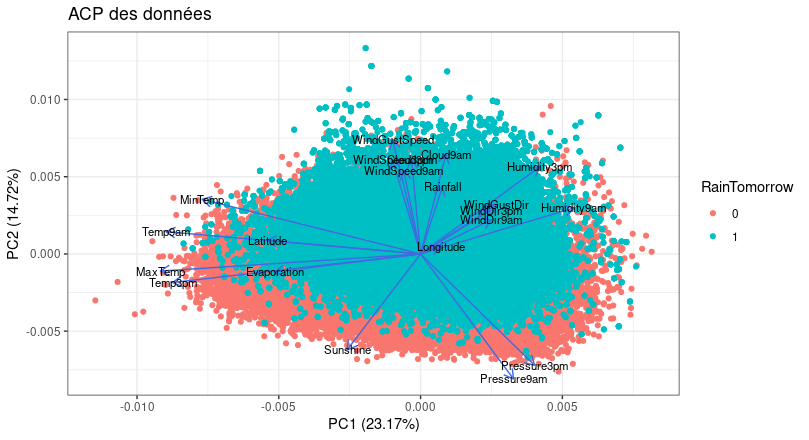
\includegraphics[width=0.8\textwidth]{Images/pca/pca_up.png}
    \caption{Analyse en Composantes Principales de nos données, après upsampling, points colorés en fonction de RainTomorrow.}
    \label{fig:pca_raintomorrow_up}
\end{figure}

\subsection{Impact sur les performances de la régression logistique}

Cette fois-ci, pour la régression linéaire, on trouve une \emph{Balanced Accuracy} de 77\% pour les deux échantillons (pas trop de surapprentissage encore une fois), pour une sensibilité de 78\% et une spécificité de 76\%. Nous avons donc équilibré les bonnes prédictions des deux classes, et d'ailleurs nous pouvons voir que la prévalence est égale à 0.5, car nous avons exactement 50\% d'observations pour chaque classe. 

\begin{multicols}{2}
    \begin{minted}{text}
    Confusion Matrix and Statistics

          y.test
    yt.glm     0     1
         0 12874  3919
         1  3599 12554

                   Accuracy : 0.7718          
                     95% CI : (0.7672, 0.7763)
        No Information Rate : 0.5             
        P-Value [Acc > NIR] : < 2.2e-16       

                      Kappa : 0.5436          

     Mcnemar's Test P-Value : 0.0002341       

                Sensitivity : 0.7815          
                Specificity : 0.7621          
             Pos Pred Value : 0.7666          
             Neg Pred Value : 0.7772          
                 Prevalence : 0.5000          
             Detection Rate : 0.3908          
       Detection Prevalence : 0.5097          
          Balanced Accuracy : 0.7718          

           'Positive' Class : 0
    \end{minted}
\end{multicols}

\subsection{SMOTE}

\subsubsection{Principe de la méthode}

Penchons-nous alors sur la méthode SMOTE (Synthetic Minority Oversampling Technique). Cette méthode a pour but de créer de nouvelles observations dans le groupe de celles en minorité. Elle va faire en cela en traçant des lignes entre des observations proches au niveau de leurs modalités et prendre un point sur cette ligne, créant ainsi une nouvelle observation \cite{smote}. 

On peut imaginer cela en 2D sur le graphique de l'ACP. On trace une droite entre deux points très proches, et on prend un point sur cette droite. On peut alors lire la valeur de chaque variable sur les axes. Évidemment, il s'agit de faire cela en dimension n (n étant le nombre de modalités -de variables- que nous avons). De plus, la méthode fait ceci en prenant un échantillon aléatoire dans le groupe minoritaire, et en le faisant plusieurs fois.

Cette méthode est efficace car elle créé des observations qui sont cohérentes avec la réalité. Un problème qu'il peut y avoir, cependant, est que la classe majoritaire n'est pas prise en compte, et cela pose un problème pour les classes qui se superposent beaucoup. 

Nous utiliserons la méthode \emph{SMOTE} de la librairie \emph{smotefamily}.

La question que nous devons nous poser avant d'utiliser cette méthode set : que faire des variables à facteurs ? C'est ici que la technique de \emph{one-hot encoding} entre en jeu. Une fois que nous n'aurons plus que des variables à deux niveaux (0 ou 1), nous pourrons les considérer comme des variables numériques. Nous aurons ainsi des valeurs entre 0 et 1 pour ces variables, ce qui peut représenter la ressemblance de la nouvelle observation avec tel ou tel climat, telle ou telle saison. 

Nous nous retrouvons avec une base de données avec la distribution suivante : 

\begin{table}[H]
    \centering
        \begin{tabular}{|rrr|}
            \hline
            RainTomorrow & Compte & \% \\ 
            \hline
            \hline
            0 & 82367 & 54.22 \\
            1 & 69537 & 45.78 \\
            \hline
        \end{tabular}
    \caption{Distribution des valeurs de la variable RainTomorrow après SMOTE.}
\end{table}

\subsubsection{Impact sur la régression logistique}
\begin{multicols}{2}
    \begin{minted}{text}
    Confusion Matrix and Statistics
  
          y.test
    yt.glm     0     1
         0 13475  3662
         1  2998 10245
                                              
                   Accuracy : 0.7808          
                     95% CI : (0.7761, 0.7854)
        No Information Rate : 0.5422          
        P-Value [Acc > NIR] : < 2.2e-16       
                                              
                      Kappa : 0.5568          
                                              
     Mcnemar's Test P-Value : 4.506e-16       
                                              
                Sensitivity : 0.8180          
                Specificity : 0.7367          
             Pos Pred Value : 0.7863          
             Neg Pred Value : 0.7736          
                 Prevalence : 0.5422          
             Detection Rate : 0.4435          
       Detection Prevalence : 0.5641          
          Balanced Accuracy : 0.7773          

           'Positive' Class : 0 
                                 
    \end{minted}
\end{multicols}

Les performances sont un tout petit peu meilleures (d'un simple \%) qu'avec l'\emph{up-sampling}. Nous privilégions cependant cette méthode, car elle créé moins de redondances dans nos données. 

\subsection{Limites de la régression linéaire}

Il semblerait donc que l'on ne puisse pas faire beaucoup mieux avec la régression linéaire tout en gardant une cohérence dans les données par rapport à la réalité. Nous pouvons cependant avoir une idée des variables moins importantes dans la prédiction de la pluie en faisant une backward selection. 

On fait cette sélection grâce à la fonction \emph{step}. Cette dernière utilise pour cela le score AIC (Akaike information criterion). Finalement, nous nous sommes débarrassés des regresseurs suivants : 
\begin{itemize}
    \item Les variables de Climats et de Season qui étaient "superflues" (dû à notre façon d'avoir fait le \emph{one-hot encoding}, nous avions une classe supplémentaire comme expliqué plus haut), soient les variables Season.4 et Climate.4. 
    \item Cloud9am
    \item Latitude
\end{itemize}
Pour avoir un modèle ayant les mêmes valeurs de \emph{Null deviance} et \emph{Residual deviance} (respectivement 167600 et 111918) et pour un AIC passant de 111978 à 111975. Par ailleurs, si on effectue un test de McNemar sur les deux modèles, on a une p-value de 0.04, on rejette donc l'hypothèse H0 et on peut dire au risque de 5\% que les deux modèles ont des performances différentes. Cette sélection à pas descendante semble donc nous avoir un tout petit peu coûté en performances, on passe cependant d'une \emph{Balanced Accuracy} de 0.7769 à 0.7767.

\section{Autres modèles de prédiction}

Dans cette partie nous garderons la base de données modifiée avec la méthode SMOTE. Nous le rappelons : nous avons modifié avant cela les variables à niveaux en plusieurs variables numériques (\emph{one-hot encoding}). 

\subsection{LDA et QDA}

Pour construire ces modèles, nous nous servons de la base de données après SMOTE, mais nous devons retirer les colonnes "superflues" de Climate et Season. En effet, elles sont en réalité des combinaisons linéaires de toutes les autres et sont donc colinéaires. Ceci pose un problème de stabilité pour ces deux méthodes. Nous trouvons les performances suivantes : 
\begin{table}[ht]
    \centering
    \begin{tabular}{|r|rrr|}
        \hline
        & Sensitivity & Specificity & Balanced Accuracy \\ 
        \hline
        lda & 0.82 & 0.72 & 0.77 \\ 
        qda & 0.77 & 0.78 & 0.77 \\ 
        \hline
        \hline
        lda test & 0.83 & 0.73 & 0.78 \\ 
        qda test & 0.78 & 0.78 & 0.78 \\ 
        \hline
    \end{tabular}
\end{table}

Un test de McNemar ne nous fait pas rejeter au risque de 5\% l'hypothèse de mêmes performances. On peut donc considérer qu'ils sont autant performants. Cependant, la méthode de QDA semble moins sensible au léger déséquilibre de nos données et prédit mieux les jours pour lesquels il pleut le lendemain. 

\subsection{Arbres CART}

Commençons par créer l'arbre maximal. Il est composé de 2690 feuilles, ce qui en fait un arbre très très dense. 
\begin{multicols}{2}
    \begin{minted}{text}
        Confusion Matrix and Statistics

        y.app
  y.tmax     0     1
       0 61726  5712
       1  4168 49918
                                            
                 Accuracy : 0.9187          
                   95% CI : (0.9171, 0.9202)
      No Information Rate : 0.5422          
      P-Value [Acc > NIR] : < 2.2e-16       
                                            
                    Kappa : 0.8359          
                                            
   Mcnemar's Test P-Value : < 2.2e-16       
                                            
              Sensitivity : 0.9367          
              Specificity : 0.8973          
           Pos Pred Value : 0.9153          
           Neg Pred Value : 0.9229          
               Prevalence : 0.5422          
           Detection Rate : 0.5079          
     Detection Prevalence : 0.5549          
        Balanced Accuracy : 0.9170          
                                            
         'Positive' Class : 0    
    \end{minted}
    \begin{minted}{text}
        Confusion Matrix and Statistics

       y.test
yt.tmax     0     1
      0 14211  2659
      1  2262 11248
                                          
               Accuracy : 0.838           
                 95% CI : (0.8338, 0.8421)
    No Information Rate : 0.5422          
    P-Value [Acc > NIR] : < 2.2e-16       
                                          
                  Kappa : 0.673           
                                          
 Mcnemar's Test P-Value : 1.651e-08       
                                          
            Sensitivity : 0.8627          
            Specificity : 0.8088          
         Pos Pred Value : 0.8424          
         Neg Pred Value : 0.8326          
             Prevalence : 0.5422          
         Detection Rate : 0.4678          
   Detection Prevalence : 0.5553          
      Balanced Accuracy : 0.8357          
                                          
       'Positive' Class : 0               
                              
    \end{minted}
\end{multicols}
     
On voit tout de suite que les performances sont bien meilleures : pour l'échantillon test, nous avons une \emph{balanced Accuracy} de 83.57\%. 

On peut élaguer cet arbre afin d'en avoir un à 42 feuilles (avec une valeur de $cp=0.001$). On peut donc l'afficher (Figure \ref{fig:topt}). 

\begin{figure}[htp]
    \centering
    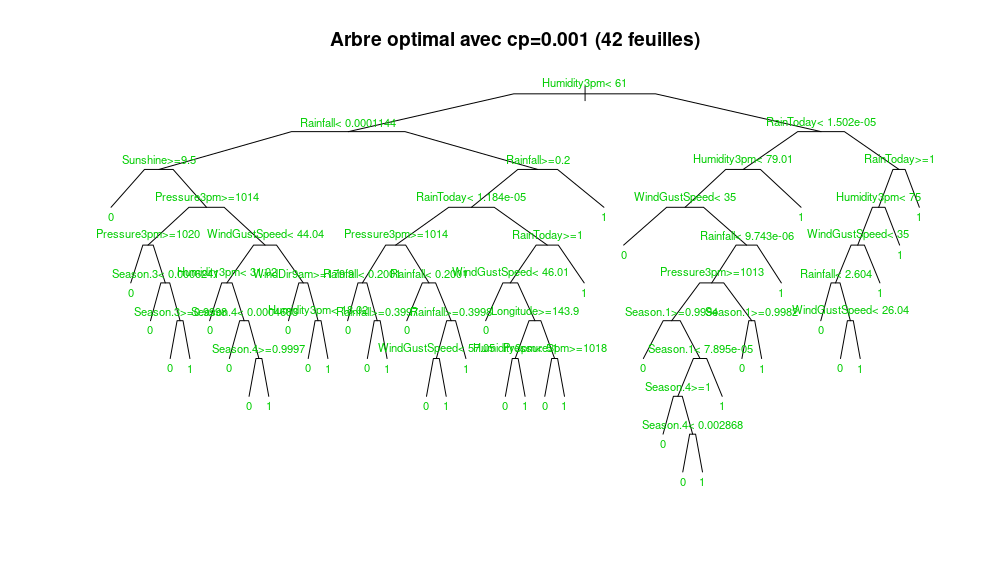
\includegraphics[width=0.8\textwidth]{Images/topt.png}
    \caption{Arbre élagué.}
    \label{fig:topt}
\end{figure}

Avec ce nombre de feuilles, on garde quand même une \emph{Balanced Accuracy} de 81.47\%, pour une sensibilité de 86.89\% et une spécificité de 76.05\%. On peut aussi classer les variables par ordre d'importance pour ces prédictions : on voit que la plus importante de loin est Humidity3pm (comme on avait vu sur les boîtes à moustaches), Rainfall et RainToday. Les trois suivantes ont un score d'importance plus faible : il s'agit de Humidity9am, Sunshine et Temp3pm.

Les variables les moins importantes sont : Cloud9am, Season.2 (l'automne), Longitude, Evaporation, WindDir3pm, WindDir9am, Latitude, WindGustDir et toutes les variables des climats.

On retrouve les deux variables écartées par la backward selection de la régression linéaire. 

\subsection{Random Forest}

Afin de ne pas avoir de trop gros arbres lors de la construction d'un modèle de random forest, nous utilisons le paramètre \emph{maxnode}. \emph{yt.rf} correspond aux valeurs prédites sur dataTest avec \emph{maxnode = 1000} et \emph{yt.rf.big} avec \emph{maxnode = 2000}. 

\begin{multicols}{2}
    \begin{minted}{text}
Confusion Matrix and Statistics

     y.test
yt.rf     0     1
    0 14770  2516
    1  1703 11391
                                         
               Accuracy : 0.8611         
                 95% CI : (0.8572, 0.865)
    No Information Rate : 0.5422         
    P-Value [Acc > NIR] : < 2.2e-16      
                                         
                  Kappa : 0.719          
                                         
 Mcnemar's Test P-Value : < 2.2e-16      
                                         
            Sensitivity : 0.8966         
            Specificity : 0.8191         
         Pos Pred Value : 0.8544         
         Neg Pred Value : 0.8699         
             Prevalence : 0.5422         
         Detection Rate : 0.4862         
   Detection Prevalence : 0.5690         
      Balanced Accuracy : 0.8579         
                                         
       'Positive' Class : 0  
    \end{minted}
    \begin{minted}{text}
        Confusion Matrix and Statistics

        y.test
yt.rf.big     0     1
       0 15051  2345
       1  1422 11562
                                         
              Accuracy : 0.876           
                95% CI : (0.8722, 0.8797)
   No Information Rate : 0.5422          
   P-Value [Acc > NIR] : < 2.2e-16       
                                         
                 Kappa : 0.7489          
                                         
Mcnemar's Test P-Value : < 2.2e-16       
                                         
           Sensitivity : 0.9137          
           Specificity : 0.8314          
        Pos Pred Value : 0.8652          
        Neg Pred Value : 0.8905          
            Prevalence : 0.5422          
        Detection Rate : 0.4954          
  Detection Prevalence : 0.5726          
     Balanced Accuracy : 0.8725          
                                         
      'Positive' Class : 0               
                             
    \end{minted}
\end{multicols}

On voit que les performances sont similaires, en effet, un test de McNemar nous donne une p-value de $0.2881$, on ne rejette donc pas l'hypothèse de même taux de bon classement de ces deux modèles (au risque de 5\%).

\subsection{Comparaisons globales}

Nous comparons ici les sensibilités, spécificités et balanced accuracies de tous les modèles que nous avons vu. 

\begin{table}[ht]
    \centering
    \begin{tabular}{|r|rrr|}
        \hline
        & Sensitivity & Specificity & Balanced Accuracy \\ 
        \hline
        glm & 0.82 & 0.74 & 0.78 \\ 
        glm.r & 0.82 & 0.74 & 0.78 \\ 
        lda & 0.82 & 0.72 & 0.77 \\ 
        qda & 0.77 & 0.78 & 0.77 \\ 
        tmax & 0.94 & 0.90 & 0.92 \\ 
        topt & 0.88 & 0.76 & 0.82 \\ 
        rf (maxnodes = 1000) & 0.90 & 0.81 & 0.86 \\ 
        rf (maxnodes = 2000) & 0.91 & 0.83 & 0.87 \\ 
        \hline
        \hline
        glm test & 0.82 & 0.74 & 0.78 \\ 
        glm.r test & 0.82 & 0.74 & 0.78 \\ 
        lda test & 0.83 & 0.73 & 0.78 \\ 
        qda test & 0.78 & 0.78 & 0.78 \\ 
        tmax test & 0.87 & 0.81 & 0.84 \\ 
        topt test & 0.88 & 0.75 & 0.81 \\ 
        rf (maxnodes = 1000) test & 0.91 & 0.83 & 0.87 \\ 
        rf (maxnodes = 2000) test & 0.91 & 0.83 & 0.87 \\ 
        \hline
    \end{tabular}
\end{table}

On peut voir que le meilleur modèle est la Random Forest. Comme nous n'avons pas de différence de performances sur dataTest pour les deux types de modèles (avec deux valeurs de maxnodes), nous privilégierons celui avec \emph{maxnodes = 1000}. Ce dernier avait une précision "régulière" (pas celle \emph{balanced}) de 86.11\%.

\newpage
\part{Conclusion}

Dans ce projet, nous avons analysé la base de données "Rain in Australia" du site Kaggle. En résumé, nous avons trouvé une manière de compléter nos données incomplètes grâce aux données géographiques que nous avons trouvé sur en ligne. Ensuite, nous avons vu des méthodes de rééchantillonnage pour régler des problèmes de déséquilibrage. Enfin, nous avons construit quelques modèles de prédiction pour en choisir un, le plus performant : la Random Forest avec 1000 nodes maximum pour les arbres des décision, nous donnant ainsi une précision de 86.11\%. 

Sur le site Kaggle, certains obtiennent à peu près le même score que nous, mais d'autres arrivent à de meilleurs résultats. Cela peut être dû à la façon dont nous avons complété et / ou ré-échantilloné nos données. Cela peut aussi être dû au modèle : certains utilisent des réseaux de neurones. Le problème de cette dernière méthode est l'explicabilité. En effet, avec les méthodes que nous avons utilisé, nous pouvons dresser les listes des variables qui sont importantes et moins importantes dans la prédiction de la pluie, ce qui peut être plus compliqué avec un réseau de neurones. 

\newpage
\Urlmuskip=0mu plus 2mu
\printbibliography

\newpage
\part{Annexes}

\begin{figure}[htp]
    \centering
    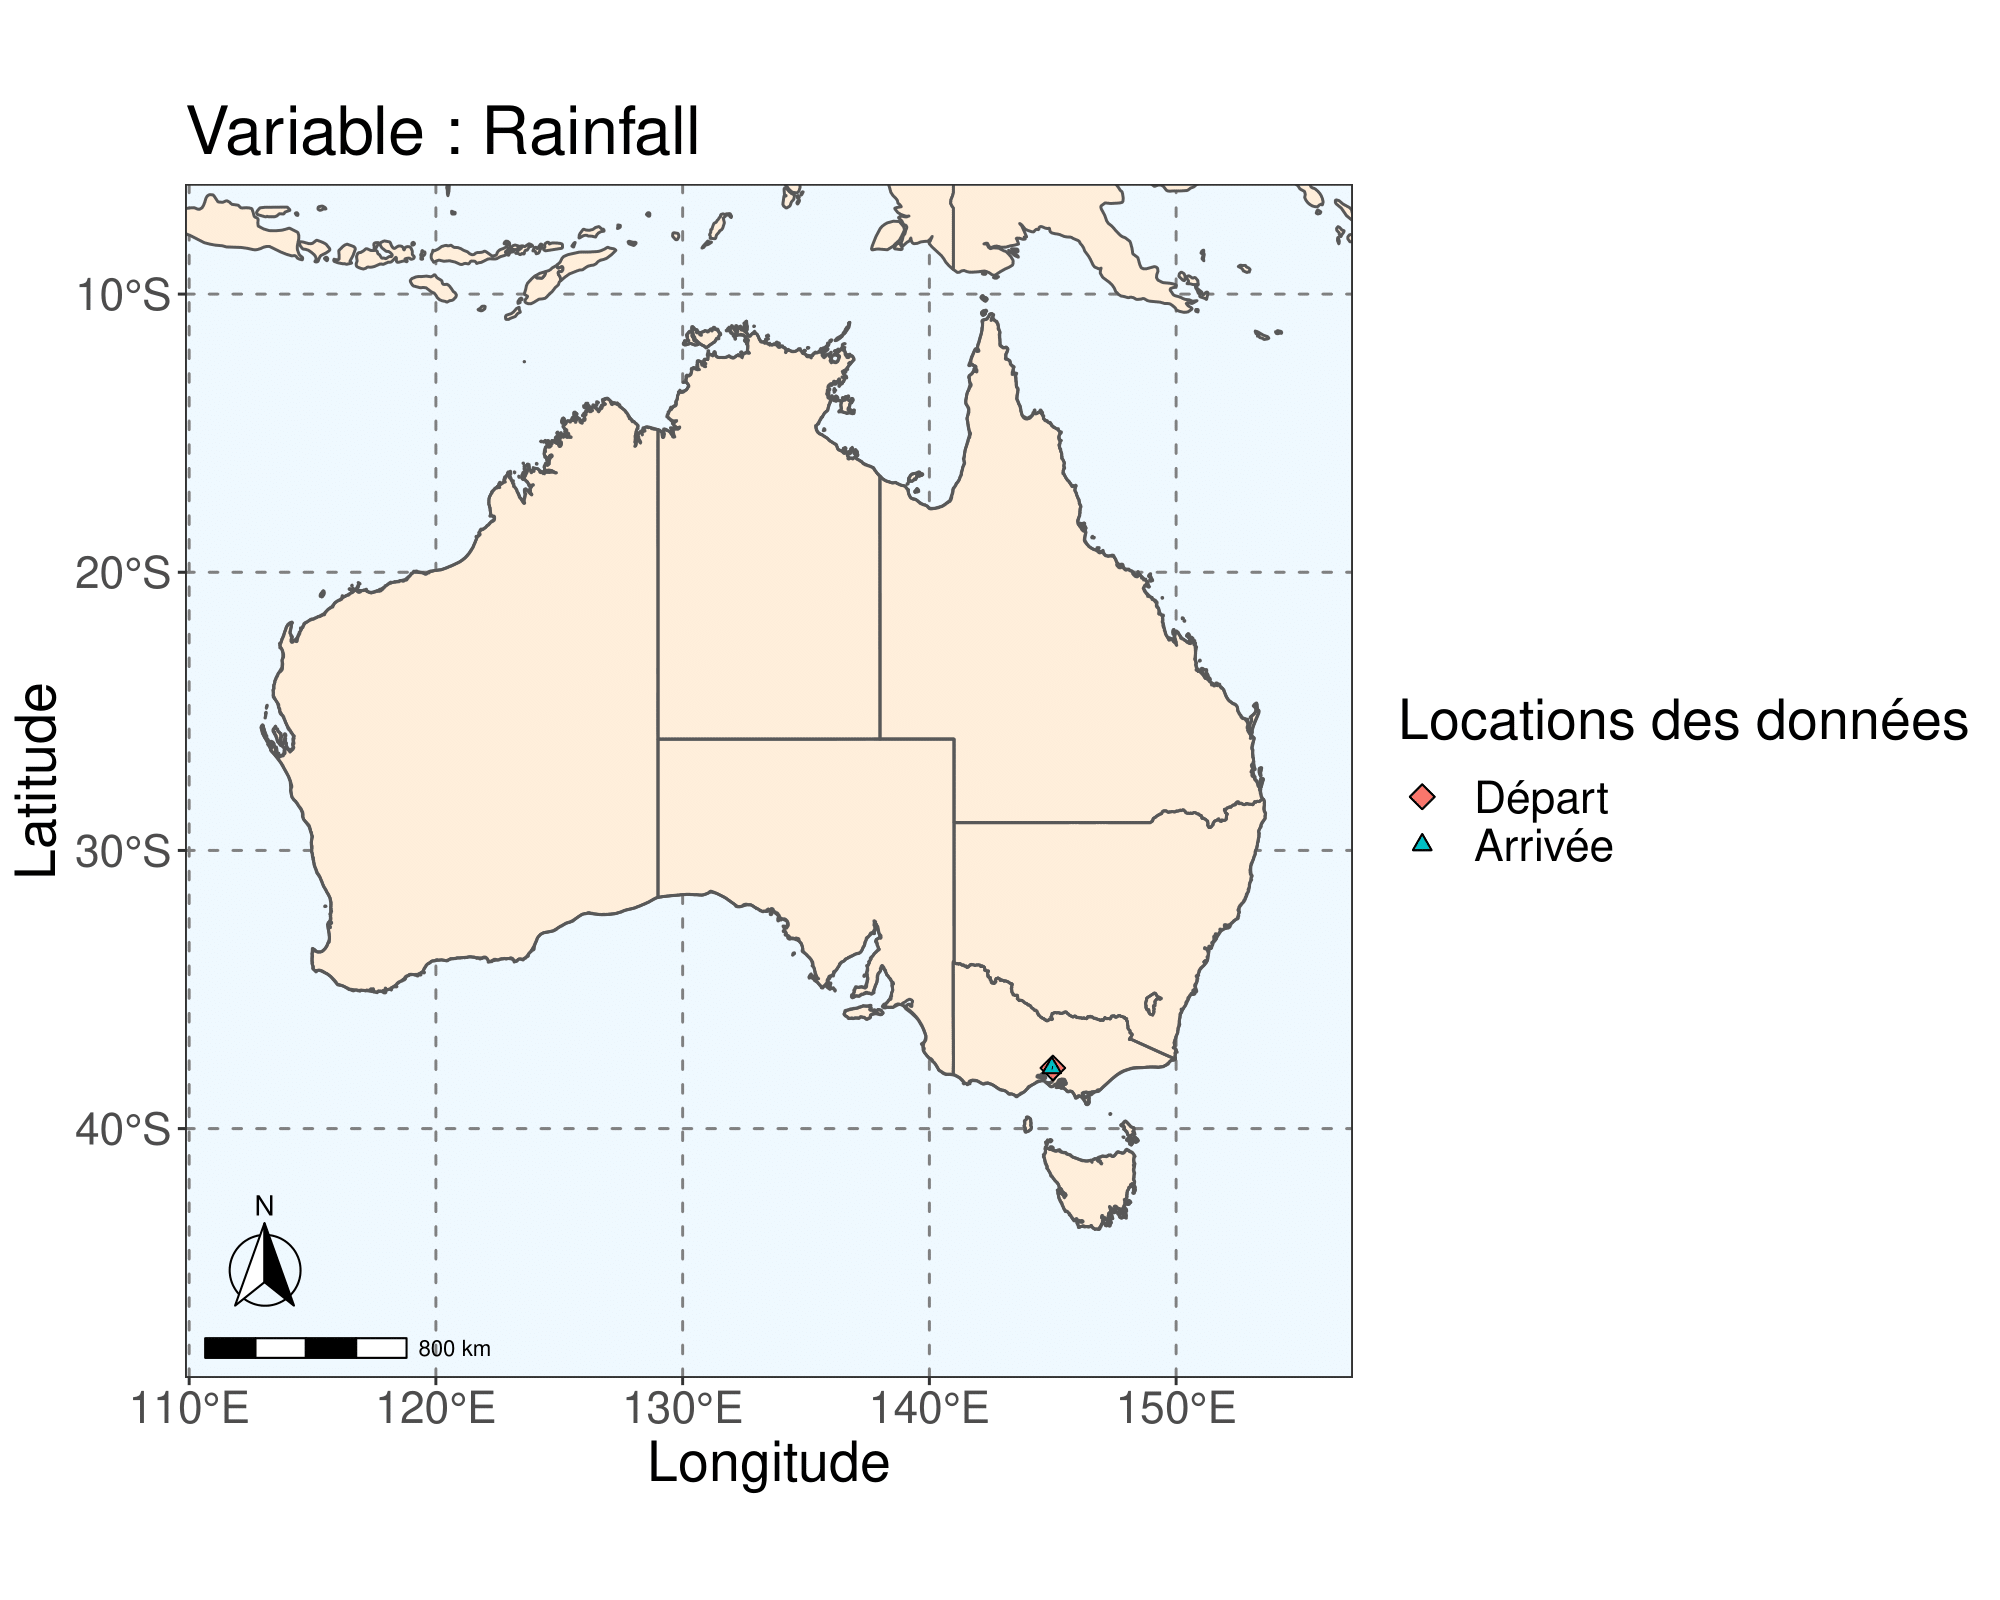
\includegraphics[width=0.45\textwidth]{Images/Australia_map_segments_complete/Australia_map_segments_complete-01.png}
    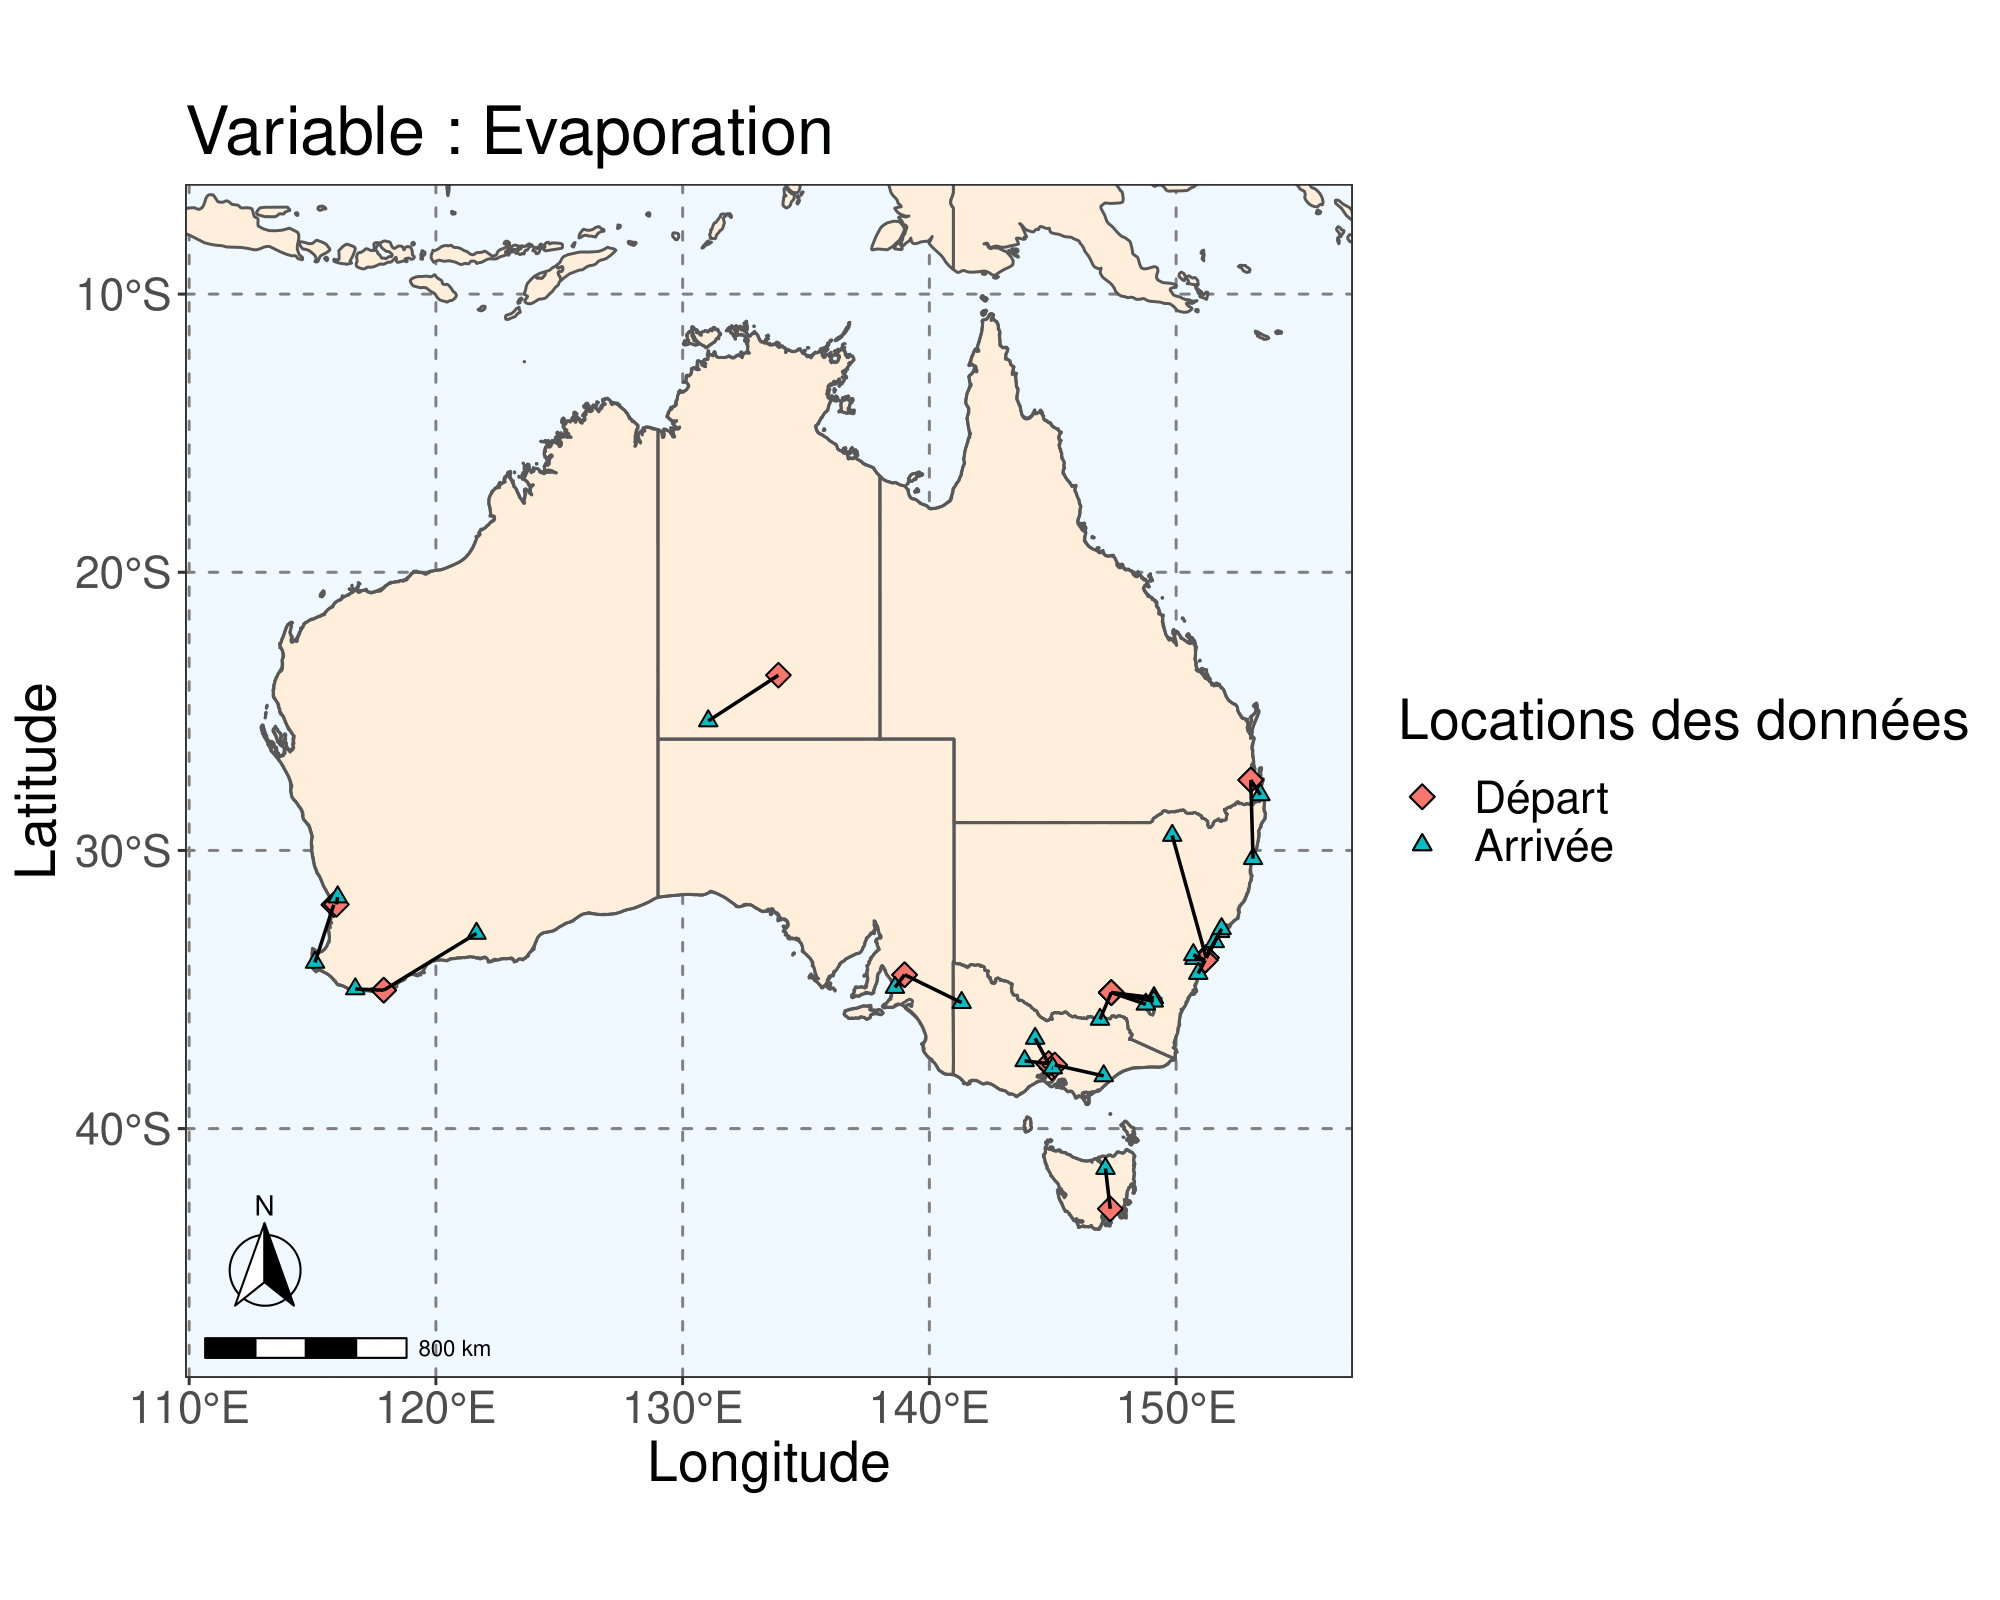
\includegraphics[width=0.45\textwidth]{Images/Australia_map_segments_complete/Australia_map_segments_complete-02.png}
    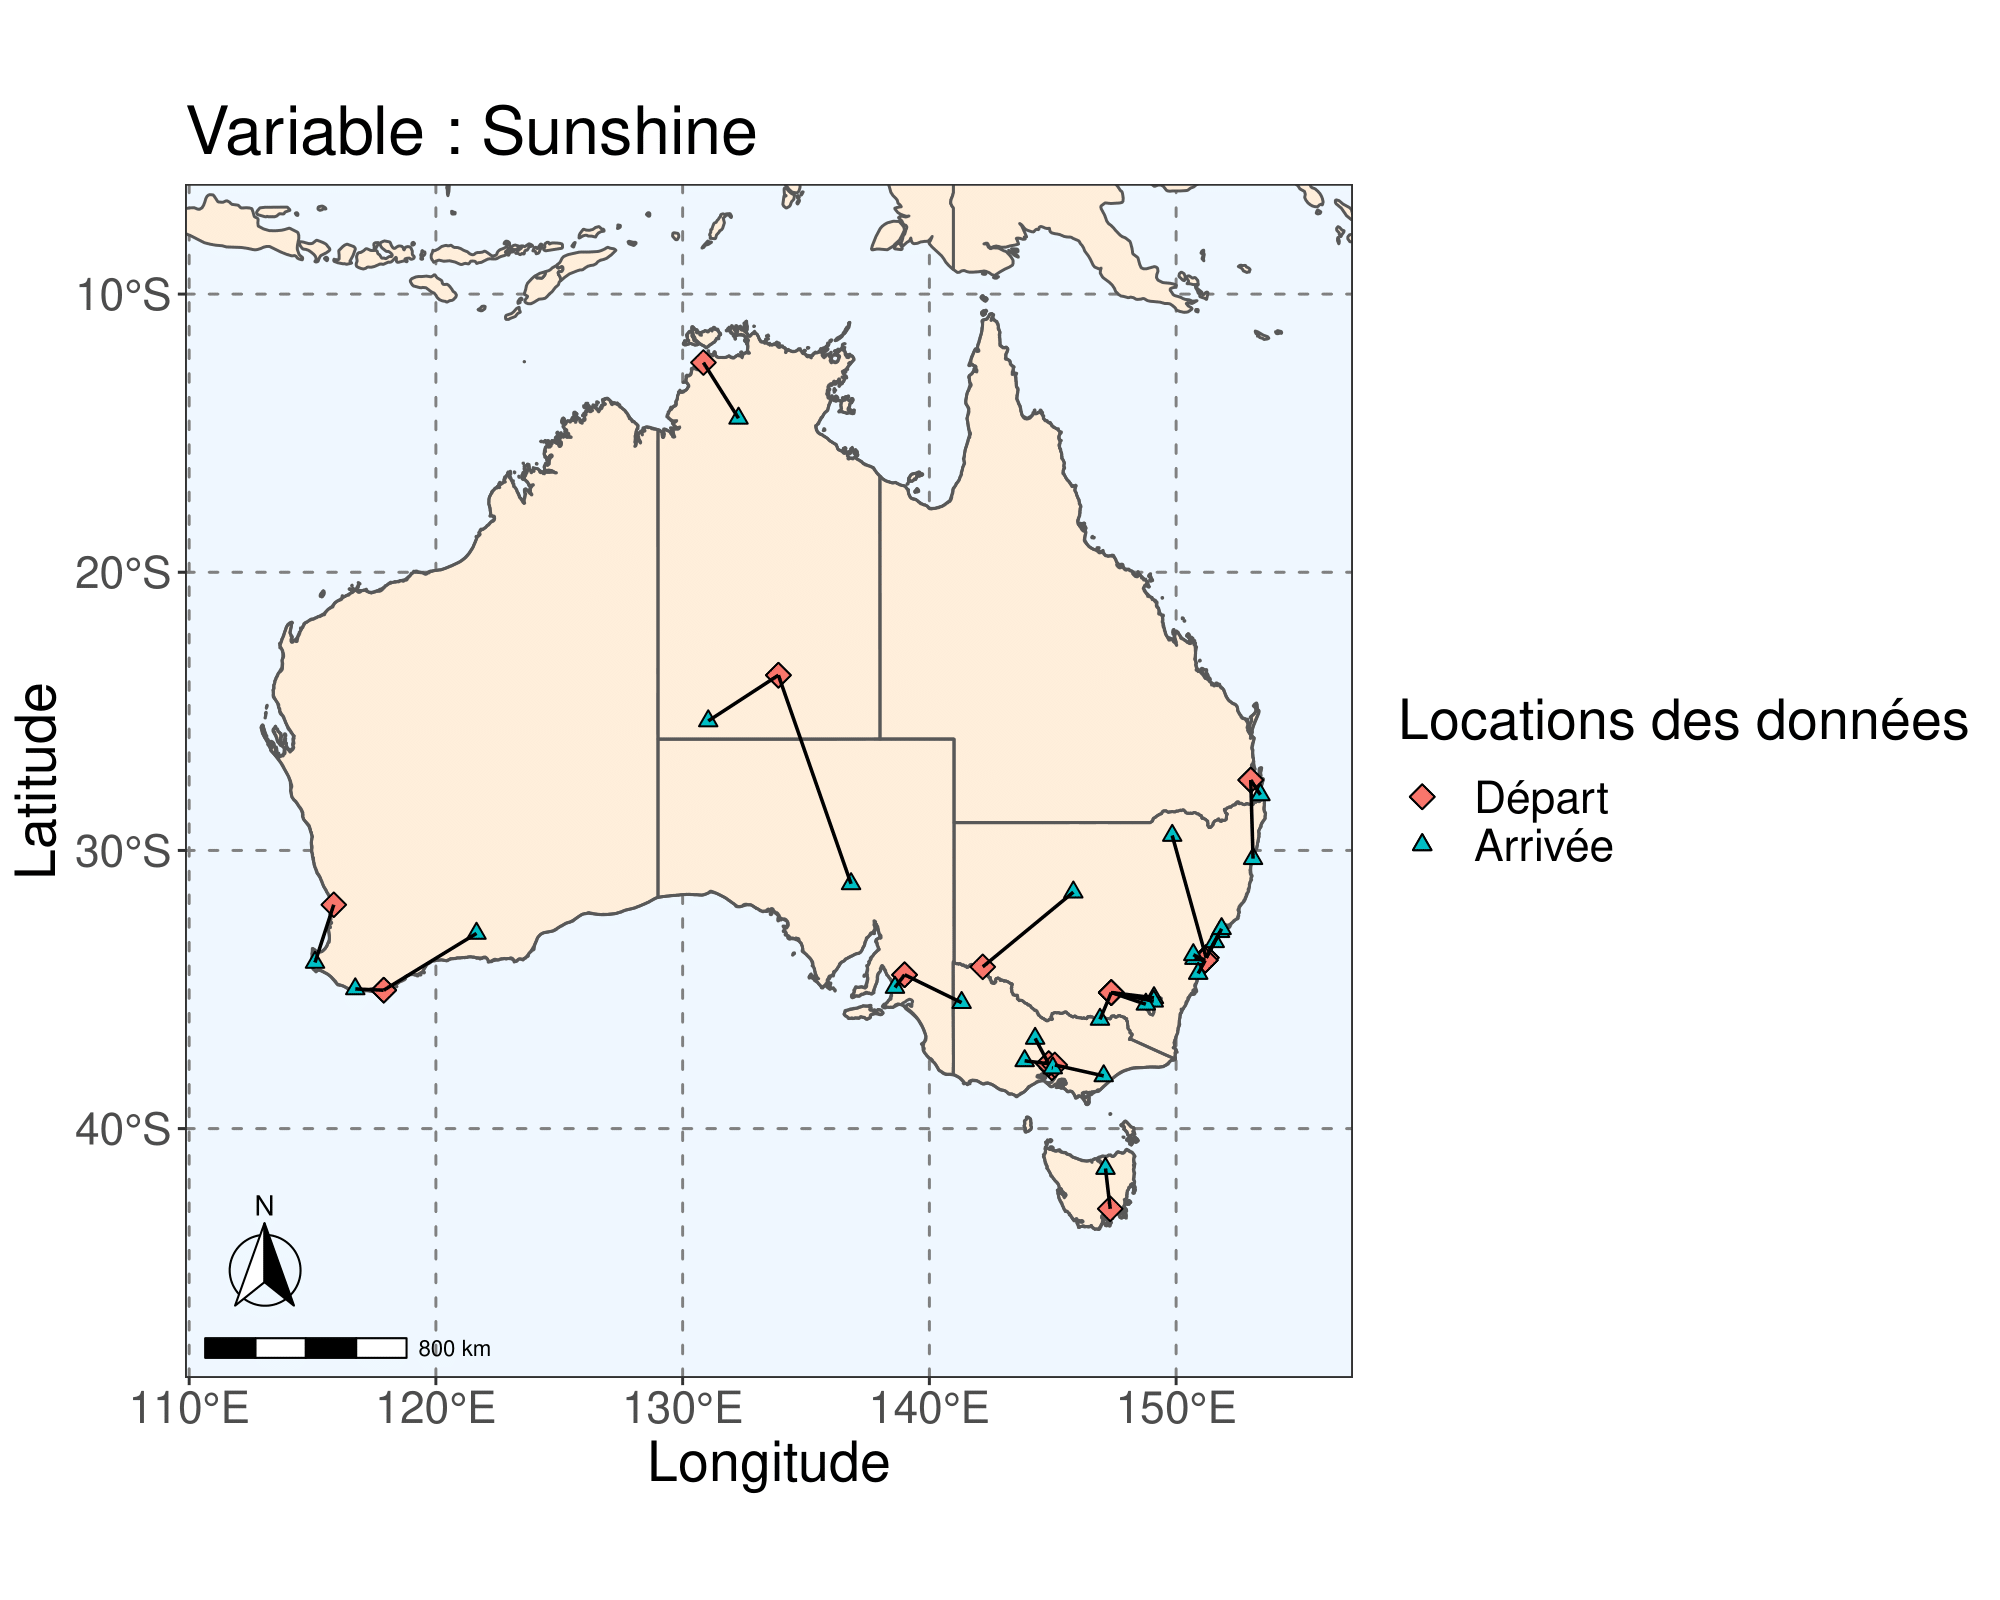
\includegraphics[width=0.45\textwidth]{Images/Australia_map_segments_complete/Australia_map_segments_complete-03.png}
    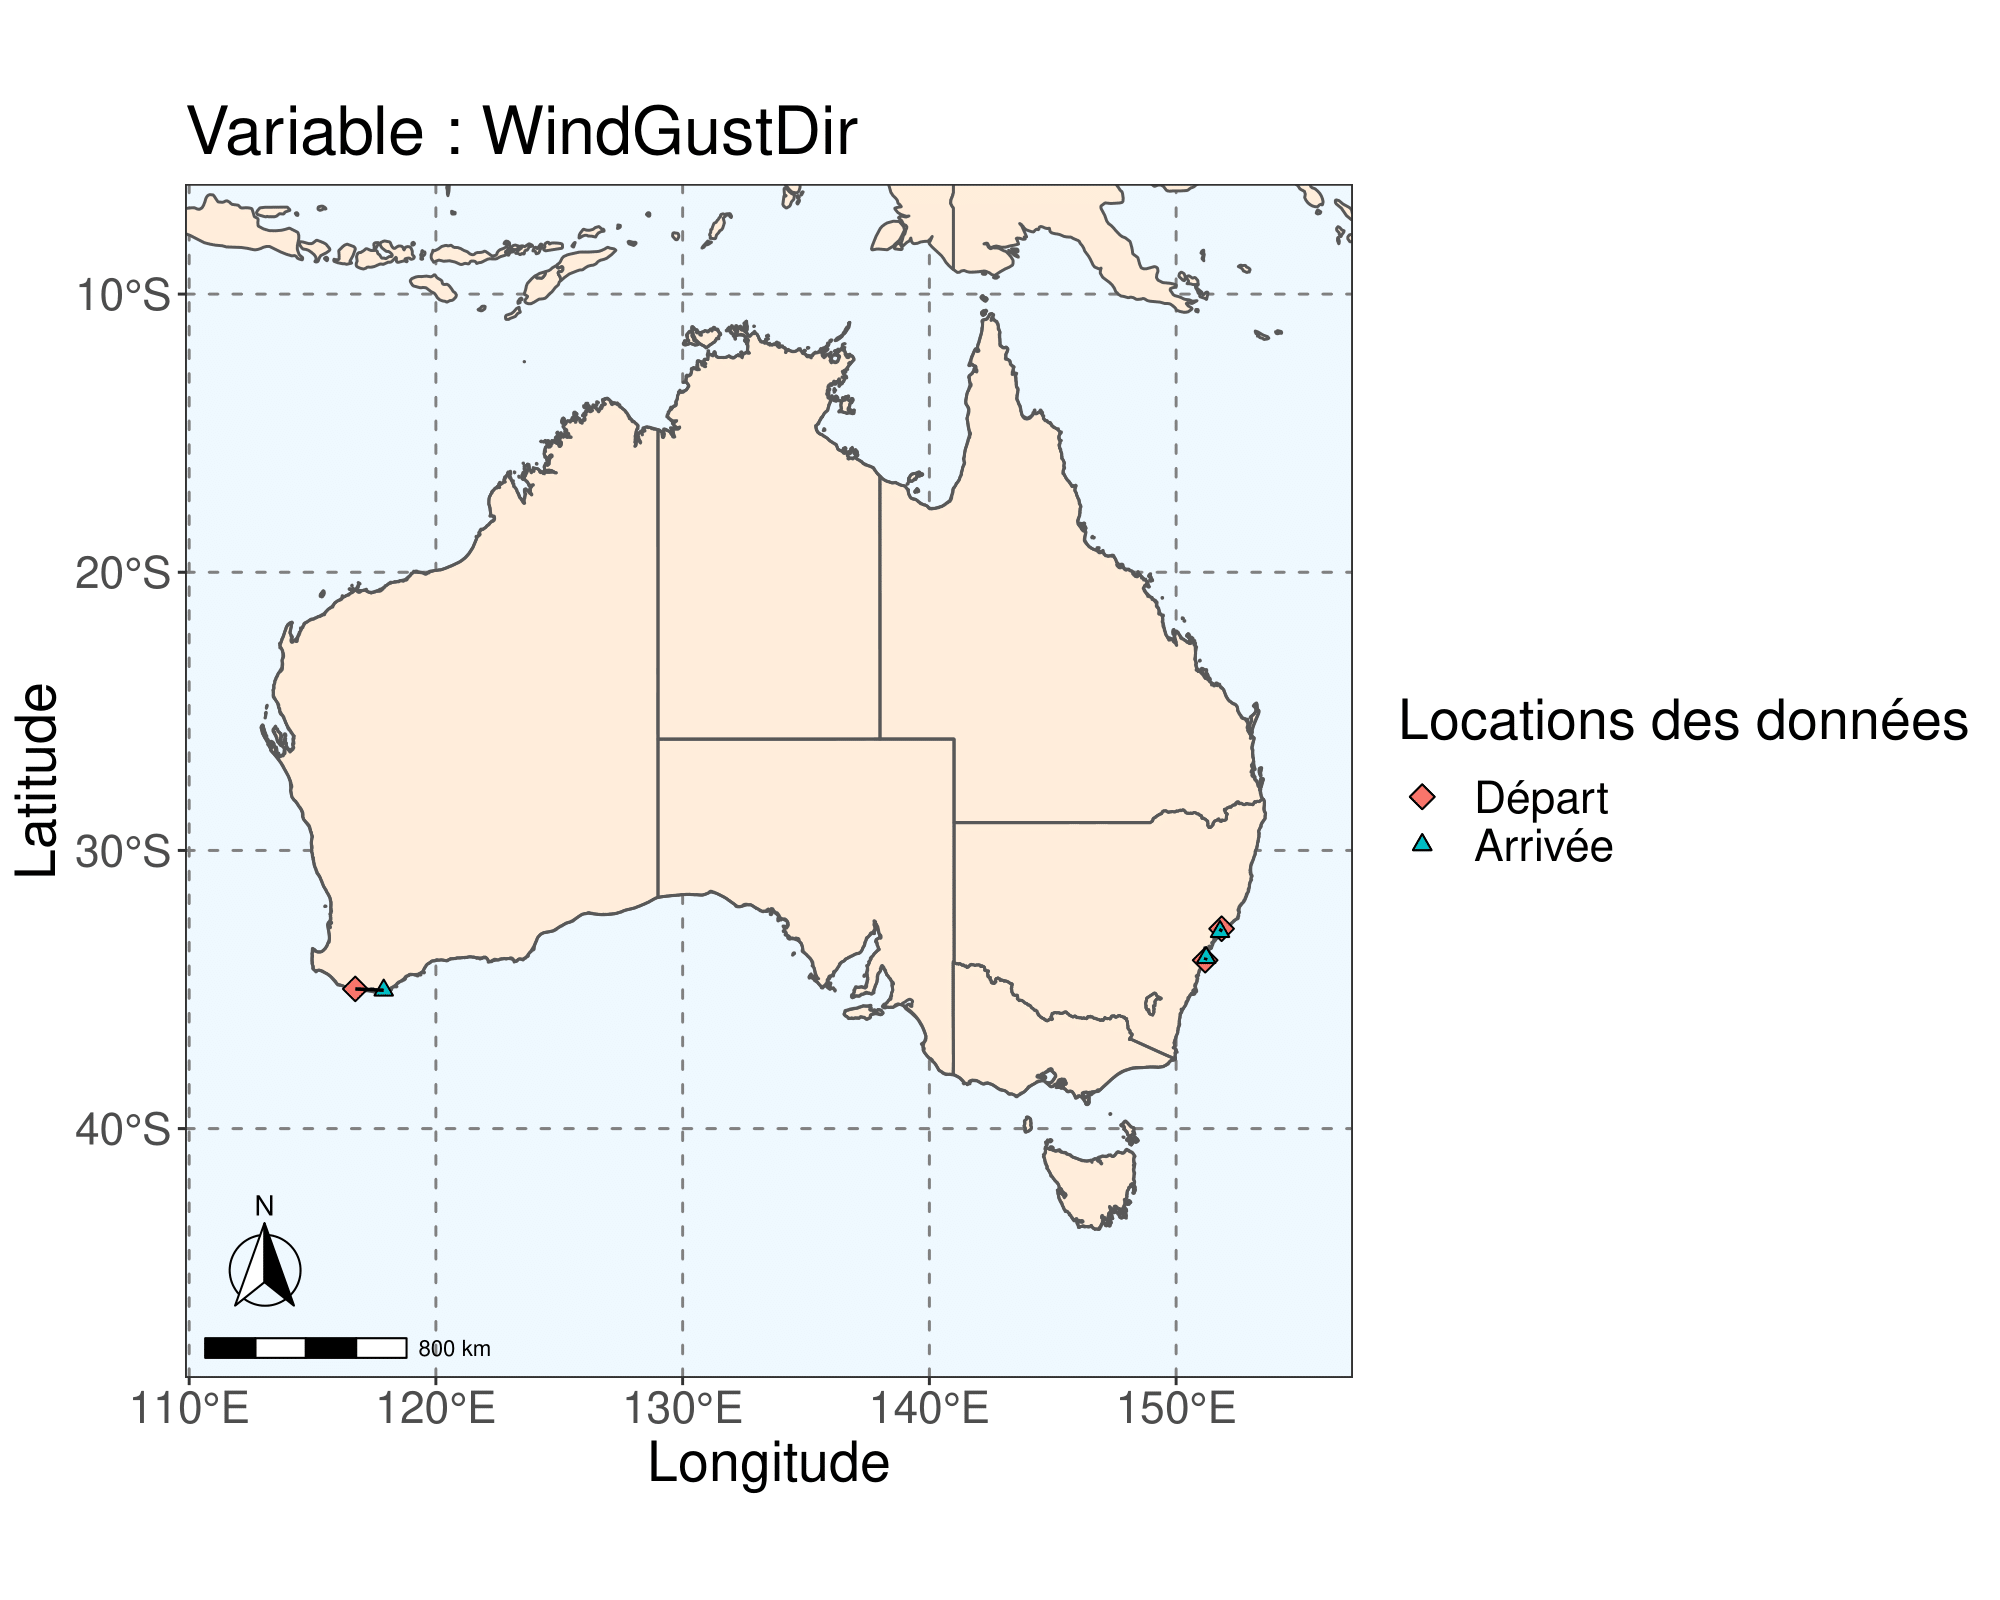
\includegraphics[width=0.45\textwidth]{Images/Australia_map_segments_complete/Australia_map_segments_complete-04.png}
    \caption{Chemin des observations copiées (ville de départ et ville(s) d'arrivée(s)) pour certaines des variables complétées 1/4.}
    \label{fig:path_data1}
\end{figure}
\begin{figure}[htp]
    \centering
    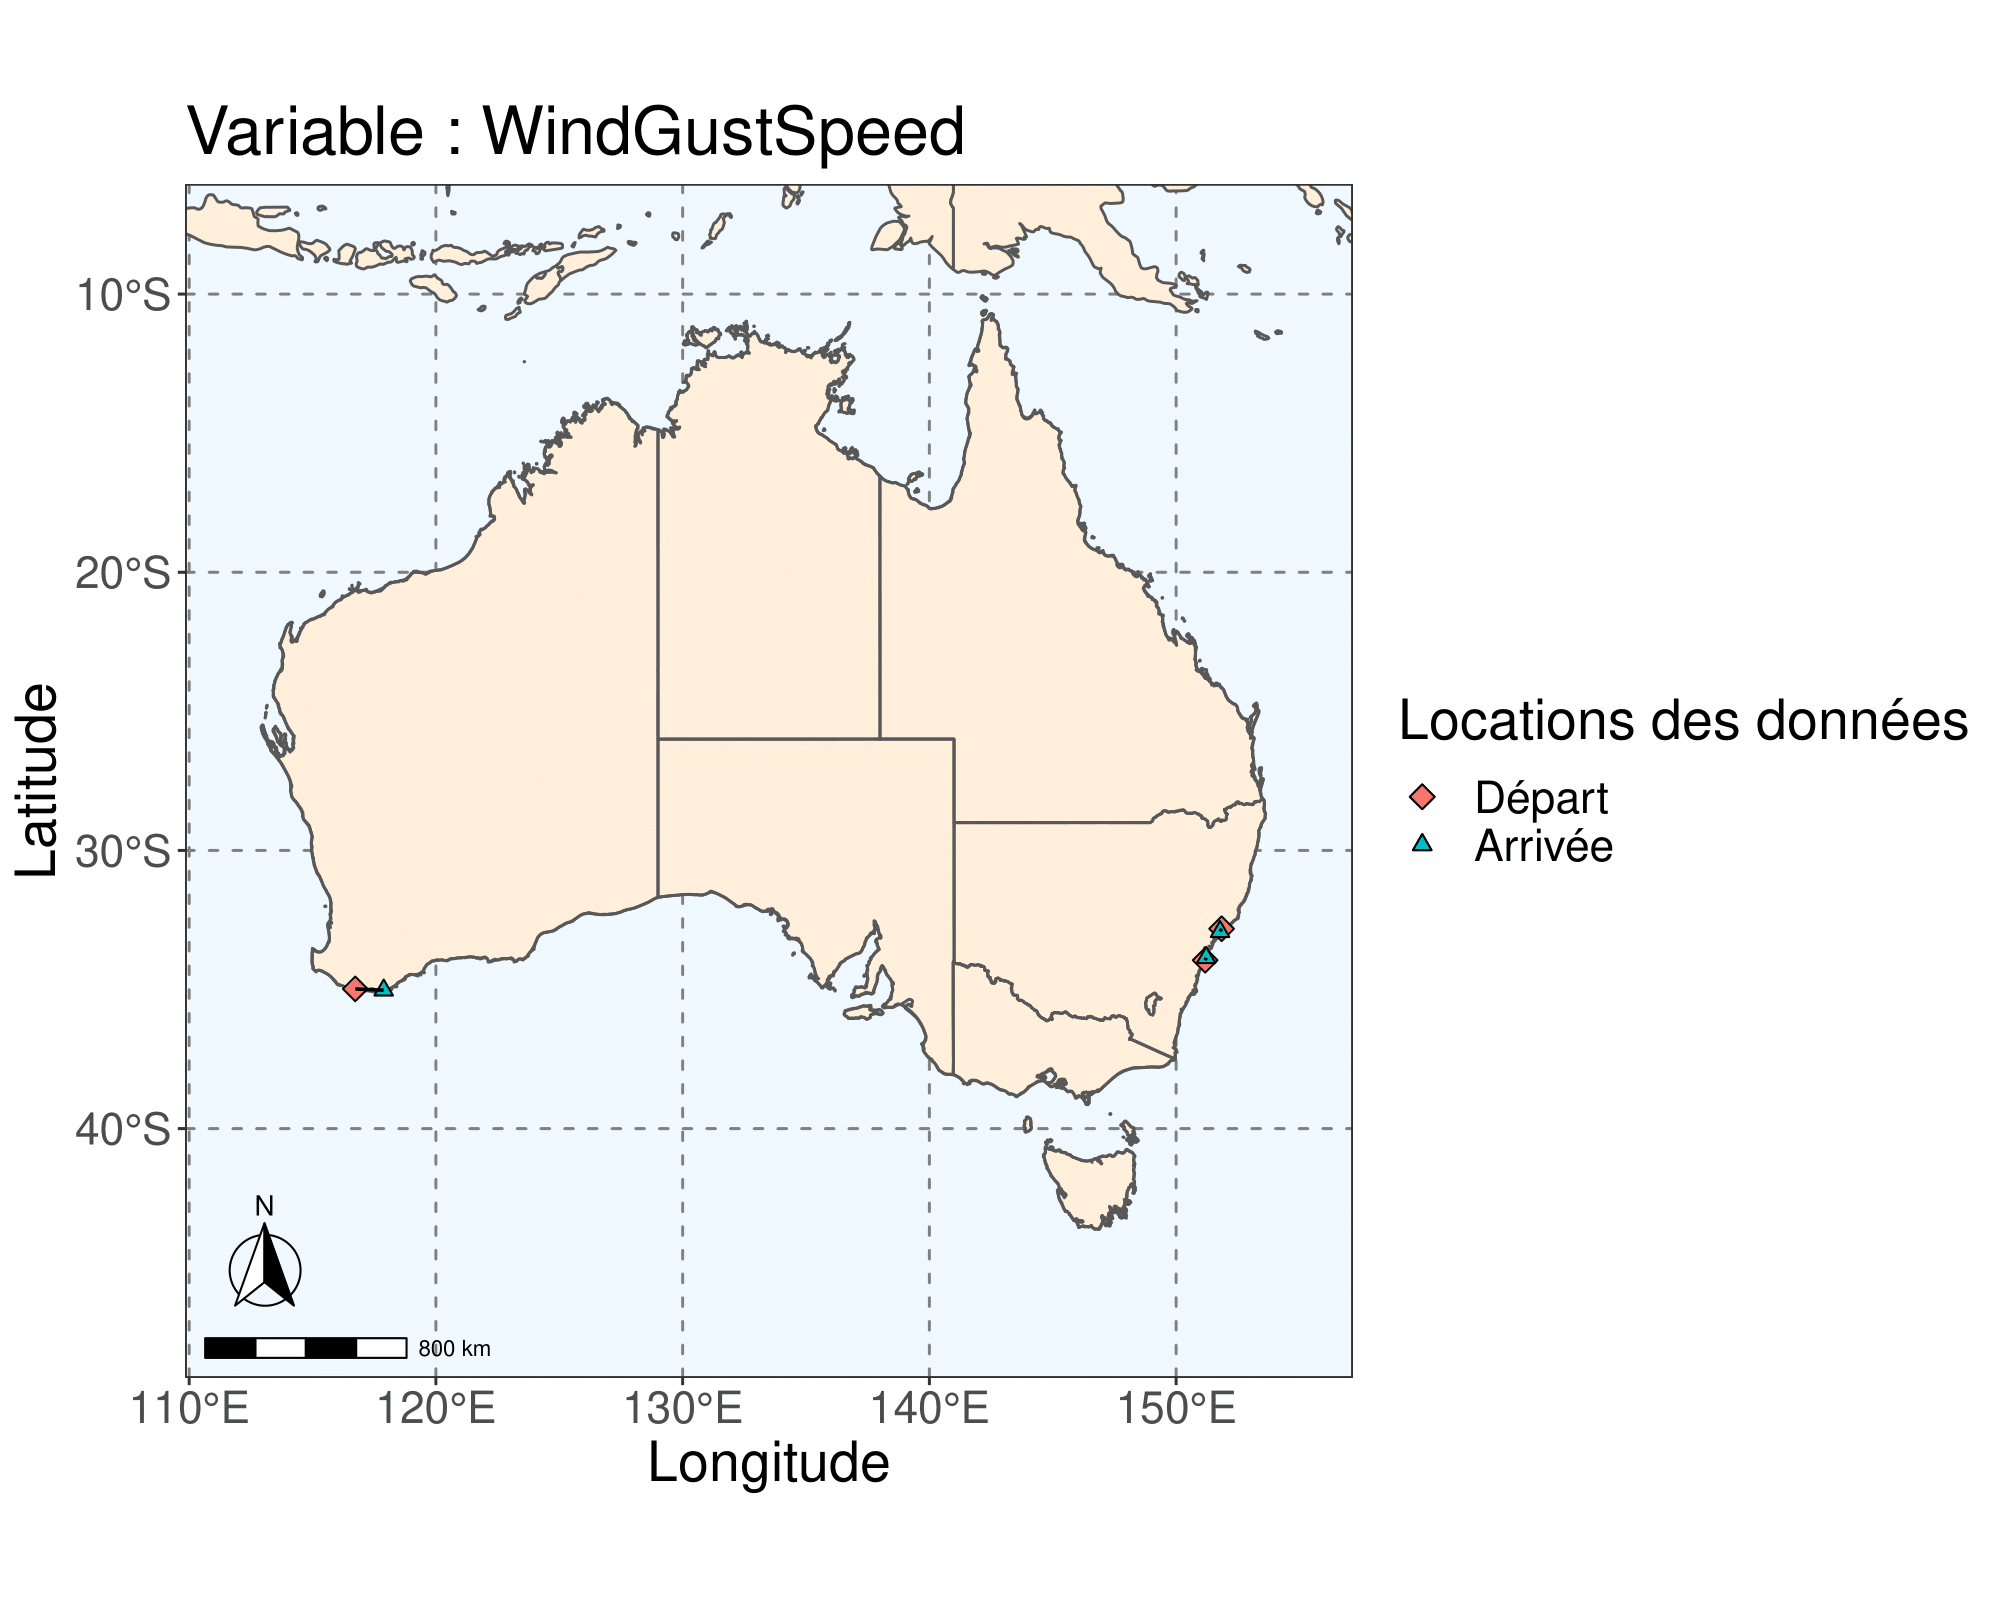
\includegraphics[width=0.45\textwidth]{Images/Australia_map_segments_complete/Australia_map_segments_complete-05.png}
    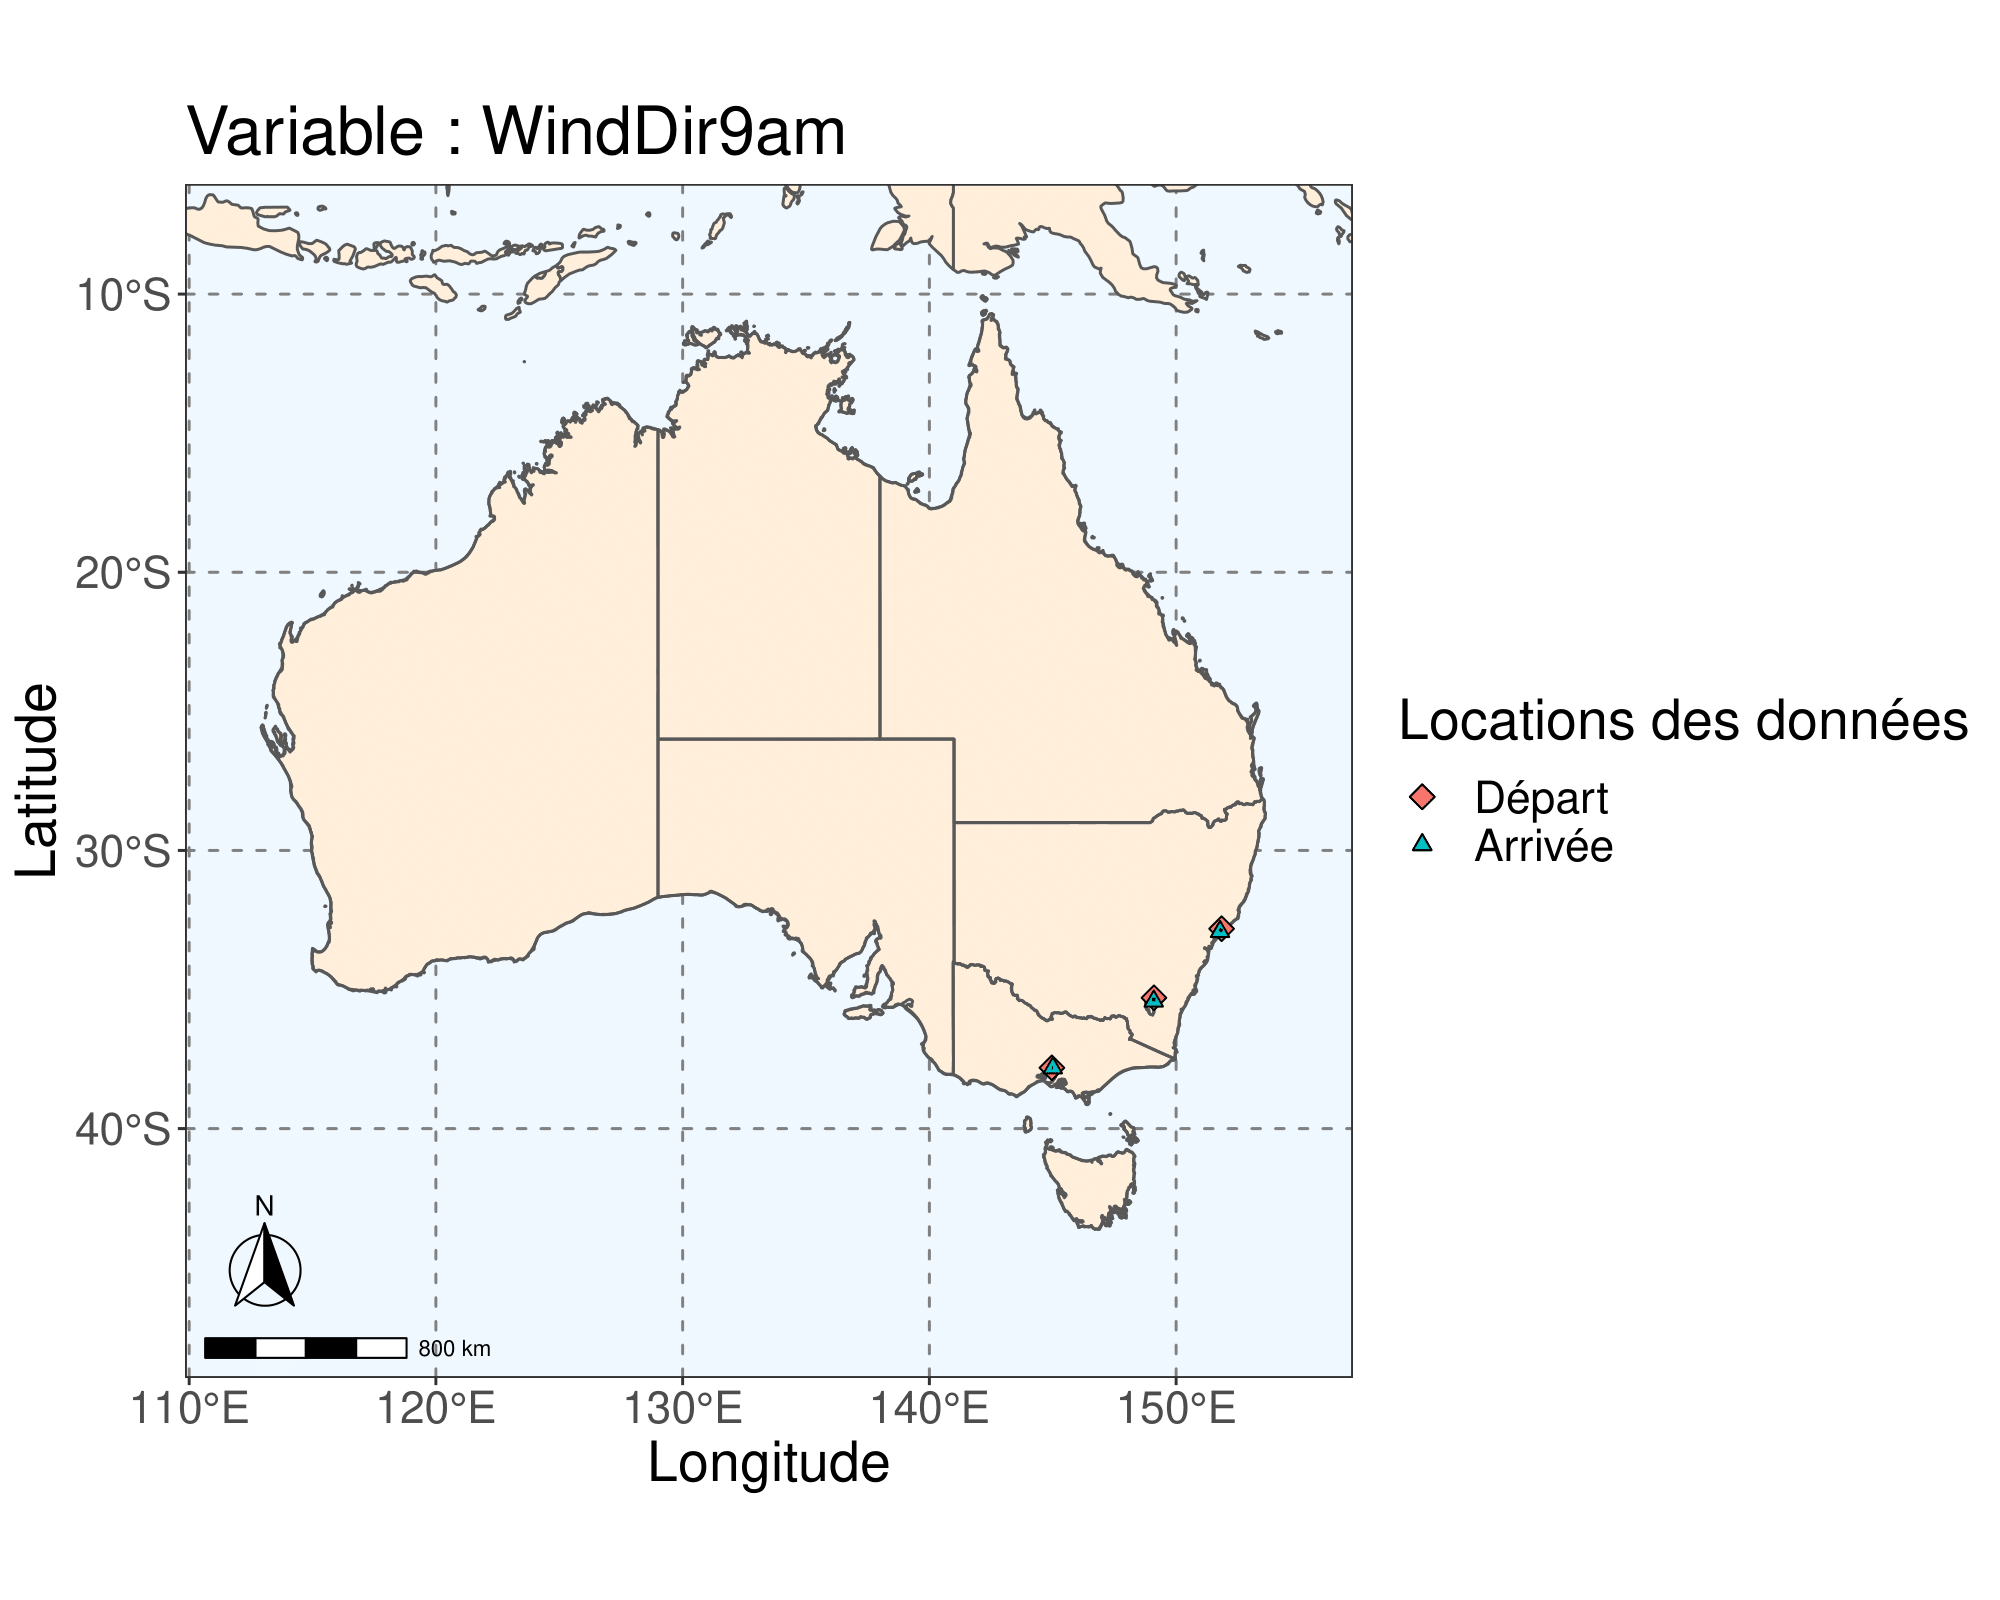
\includegraphics[width=0.45\textwidth]{Images/Australia_map_segments_complete/Australia_map_segments_complete-06.png}
    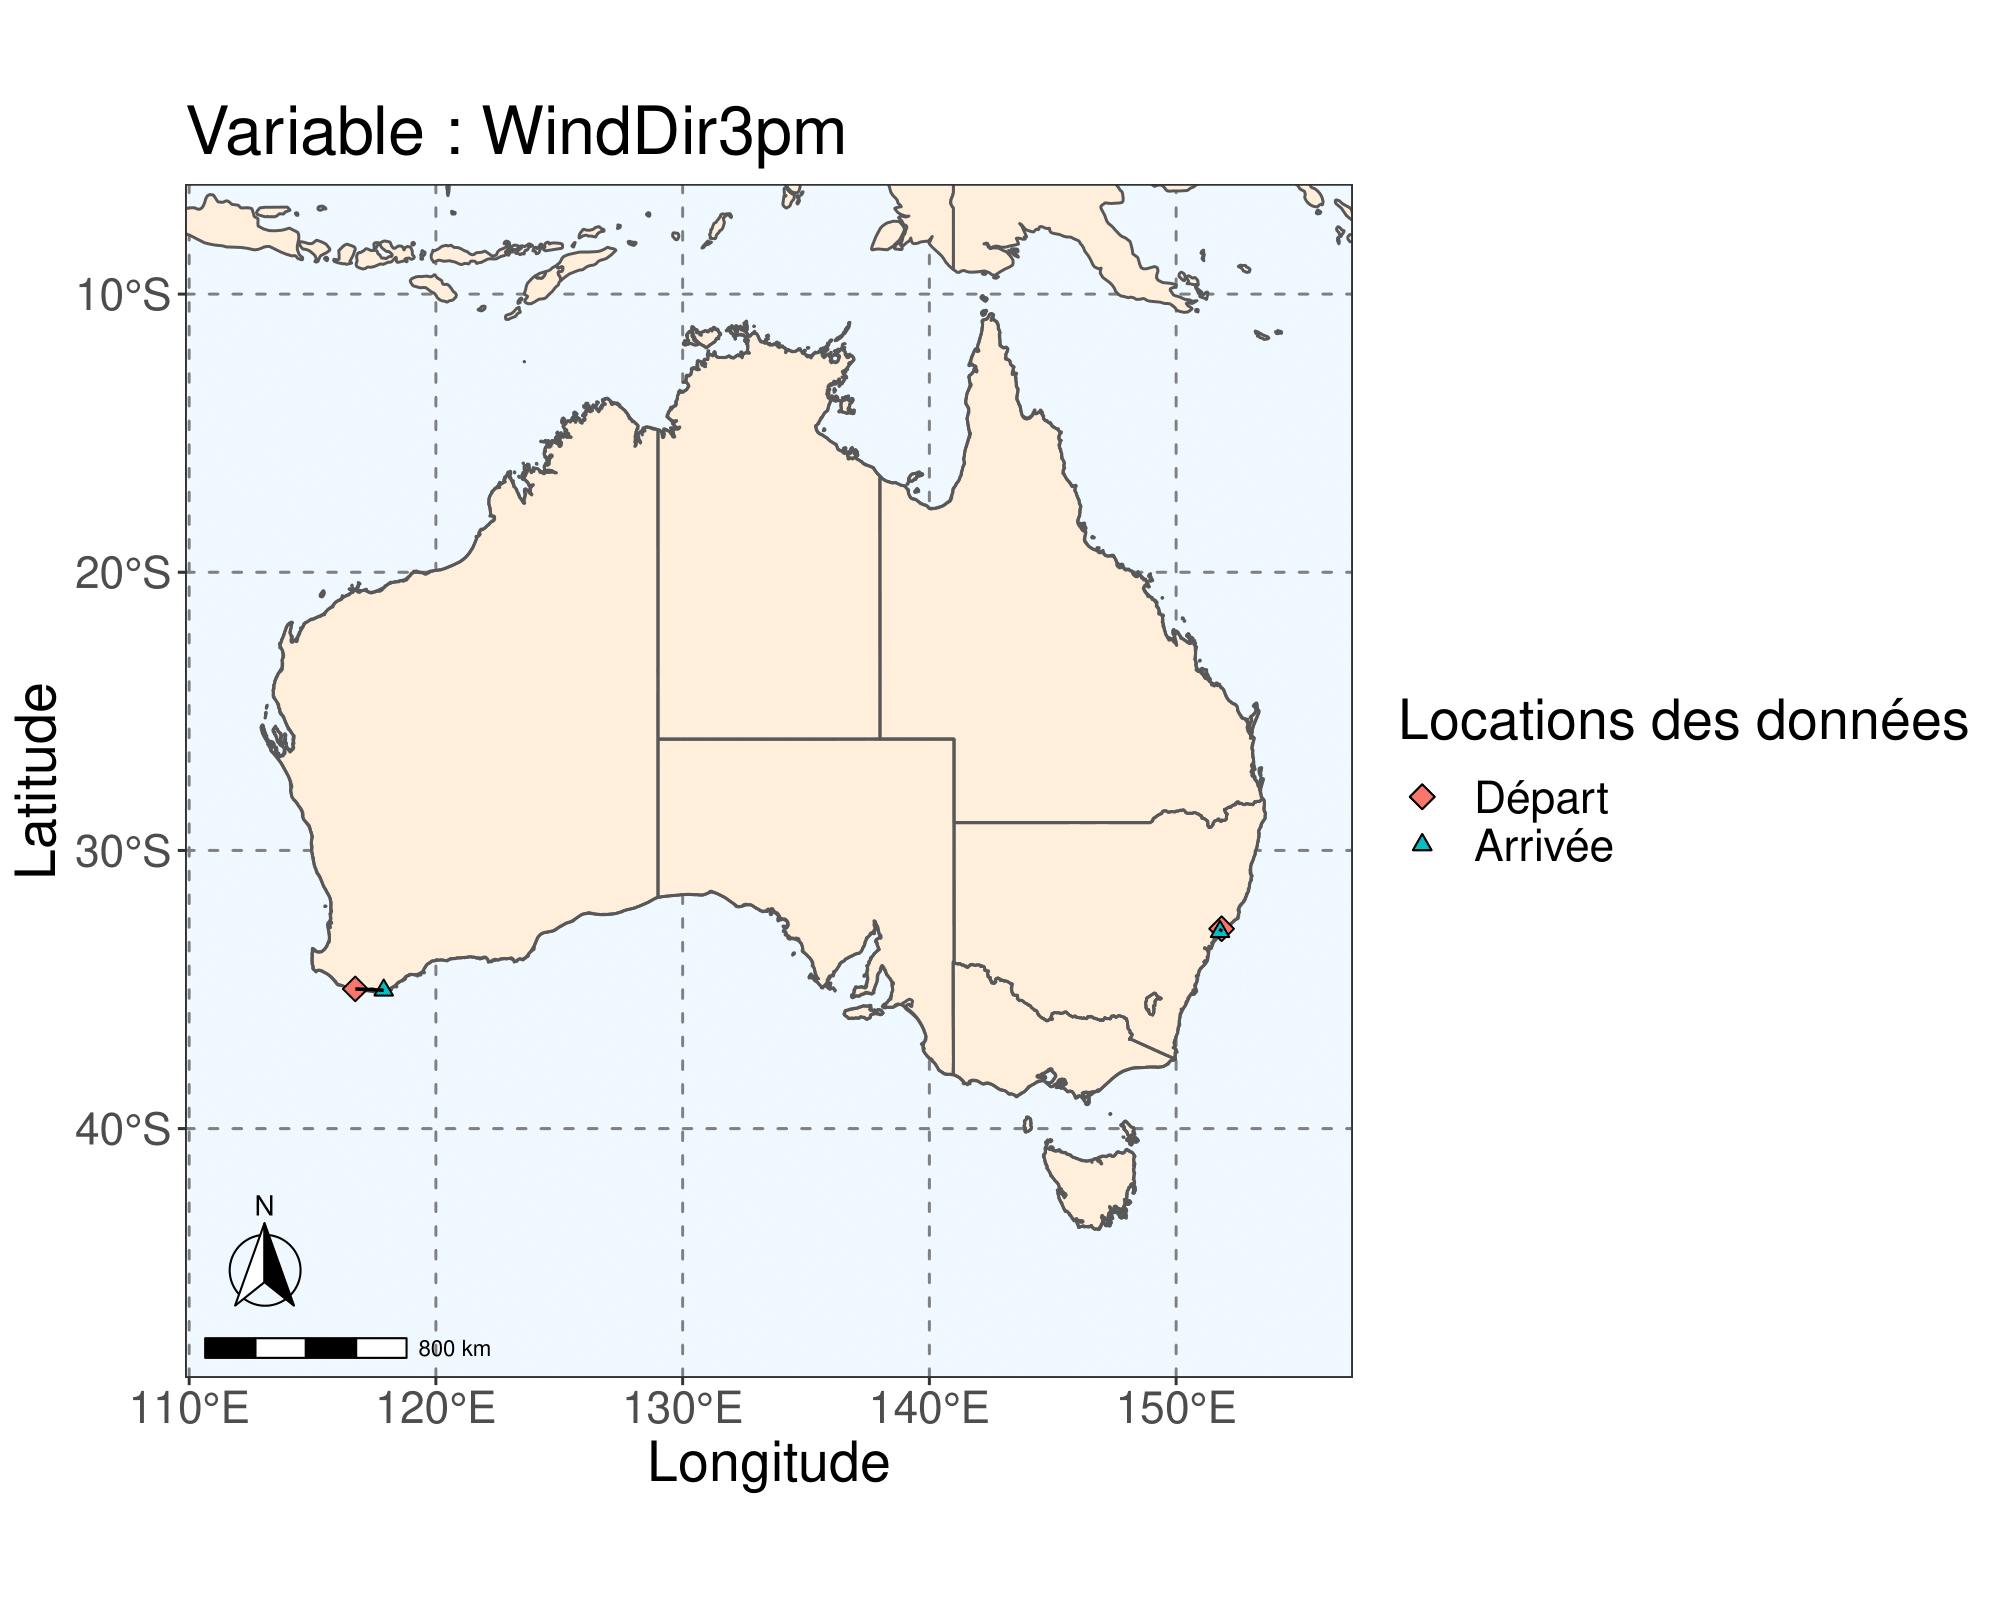
\includegraphics[width=0.45\textwidth]{Images/Australia_map_segments_complete/Australia_map_segments_complete-07.png}
    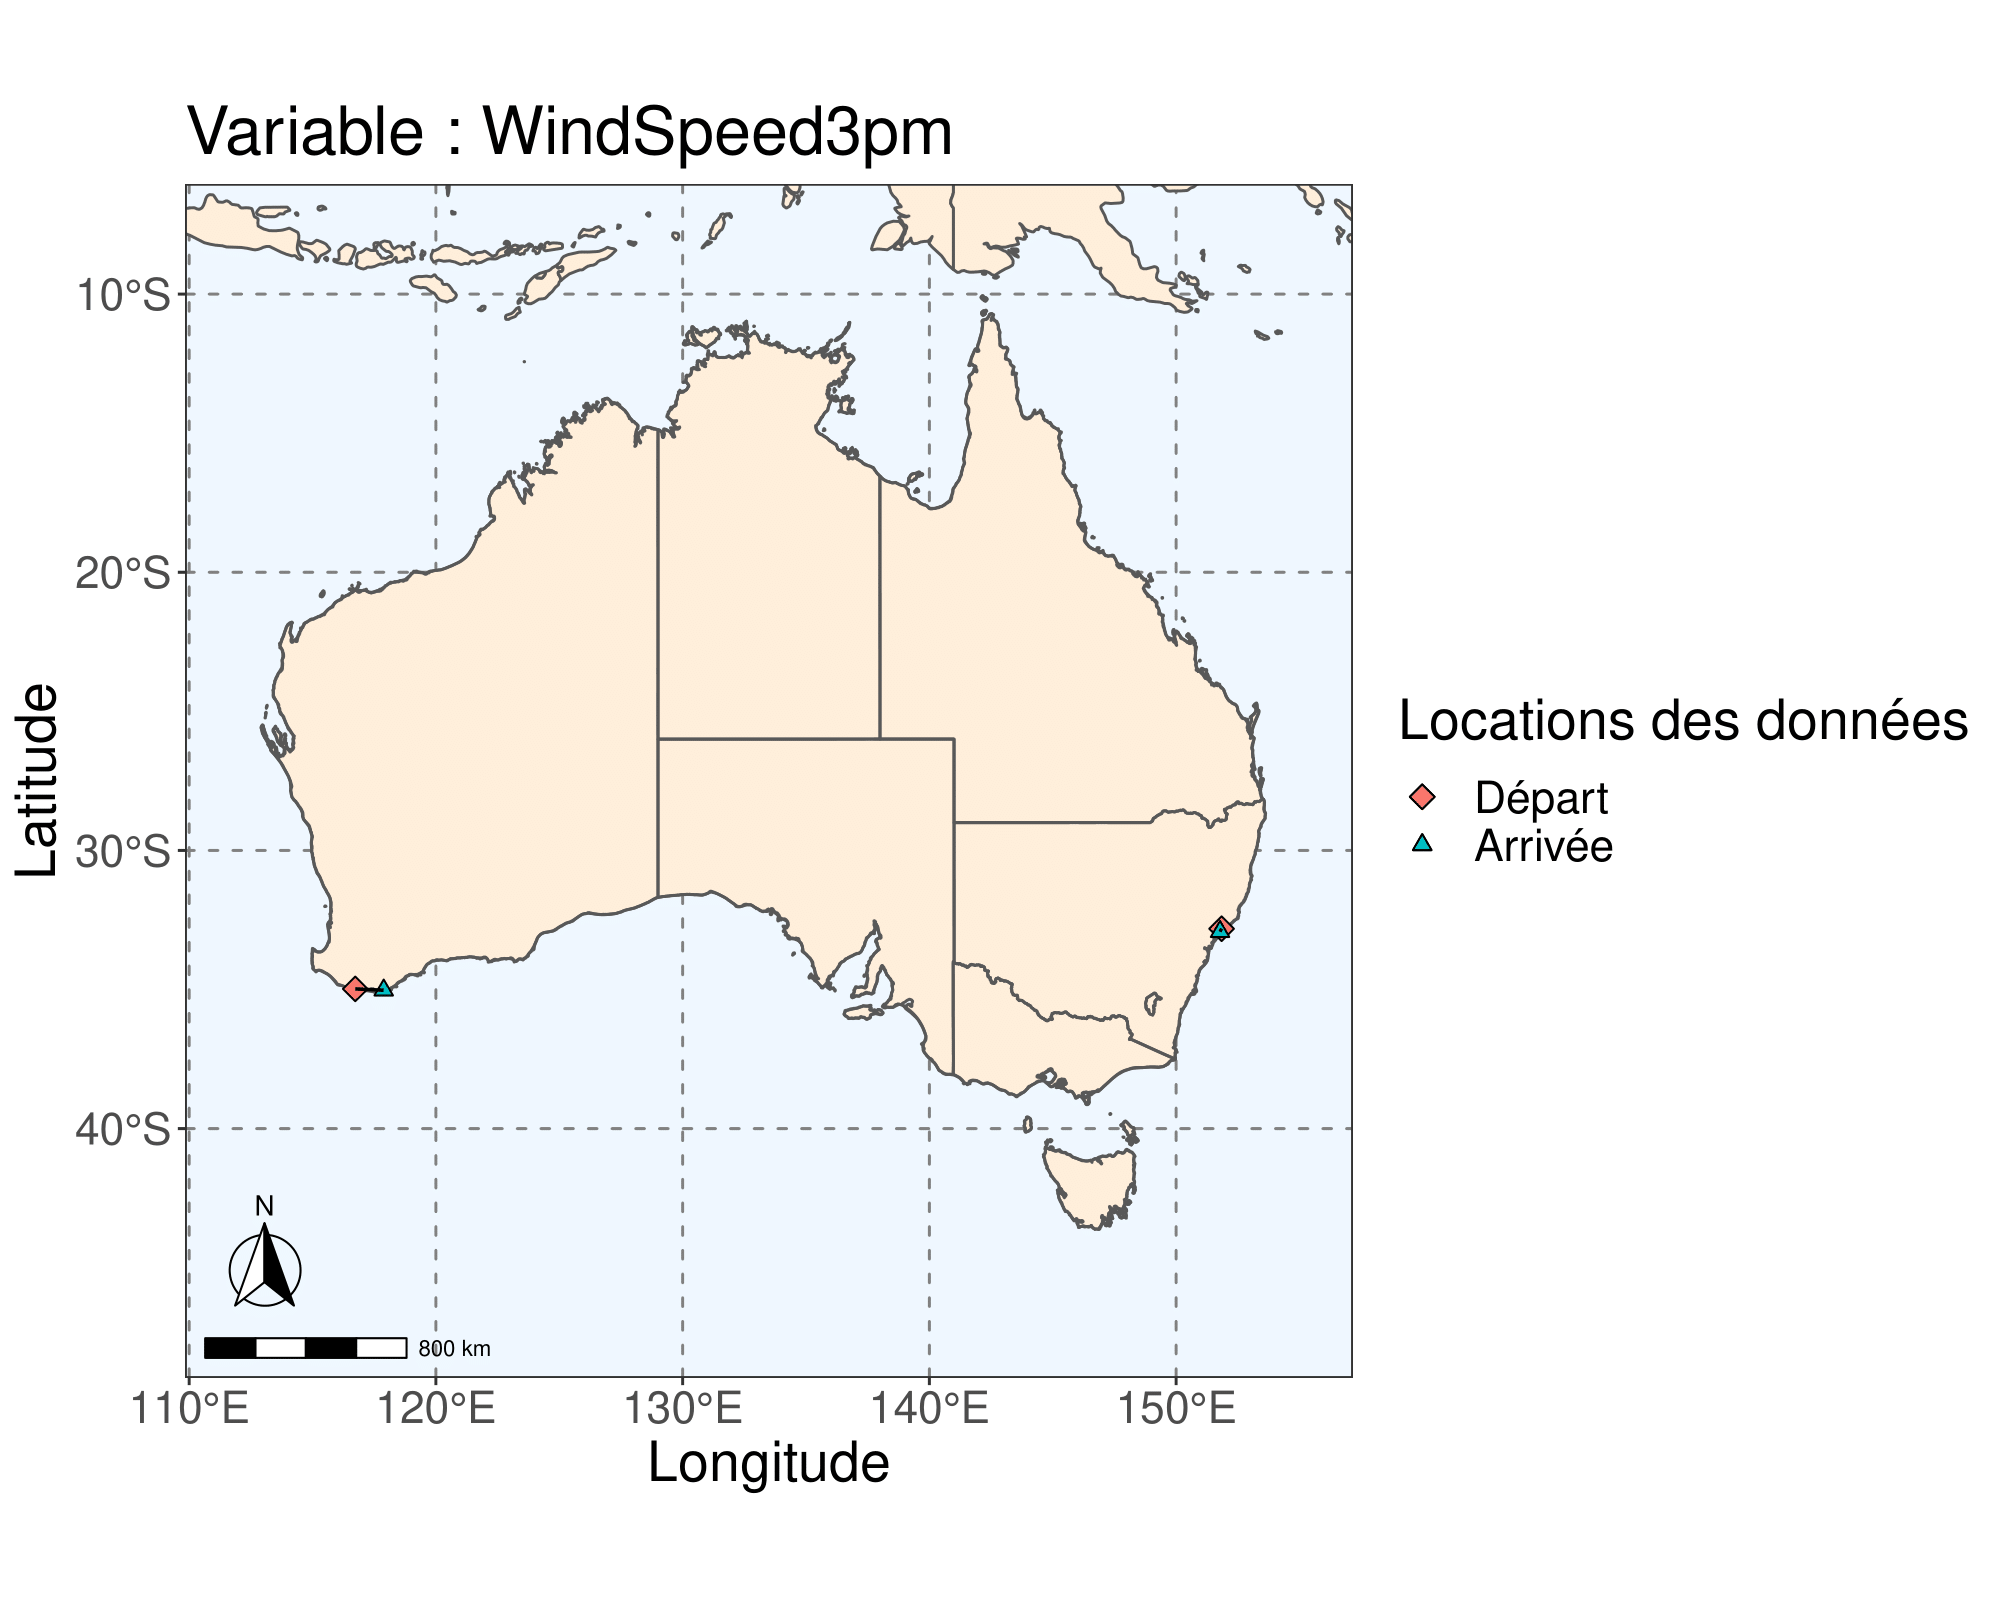
\includegraphics[width=0.45\textwidth]{Images/Australia_map_segments_complete/Australia_map_segments_complete-08.png}
    \caption{Chemin des observations copiées (ville de départ et ville(s) d'arrivée(s)) pour certaines des variables complétées 2/4.}
    \label{fig:path_data2}
\end{figure}
\begin{figure}[htp]
    \centering
    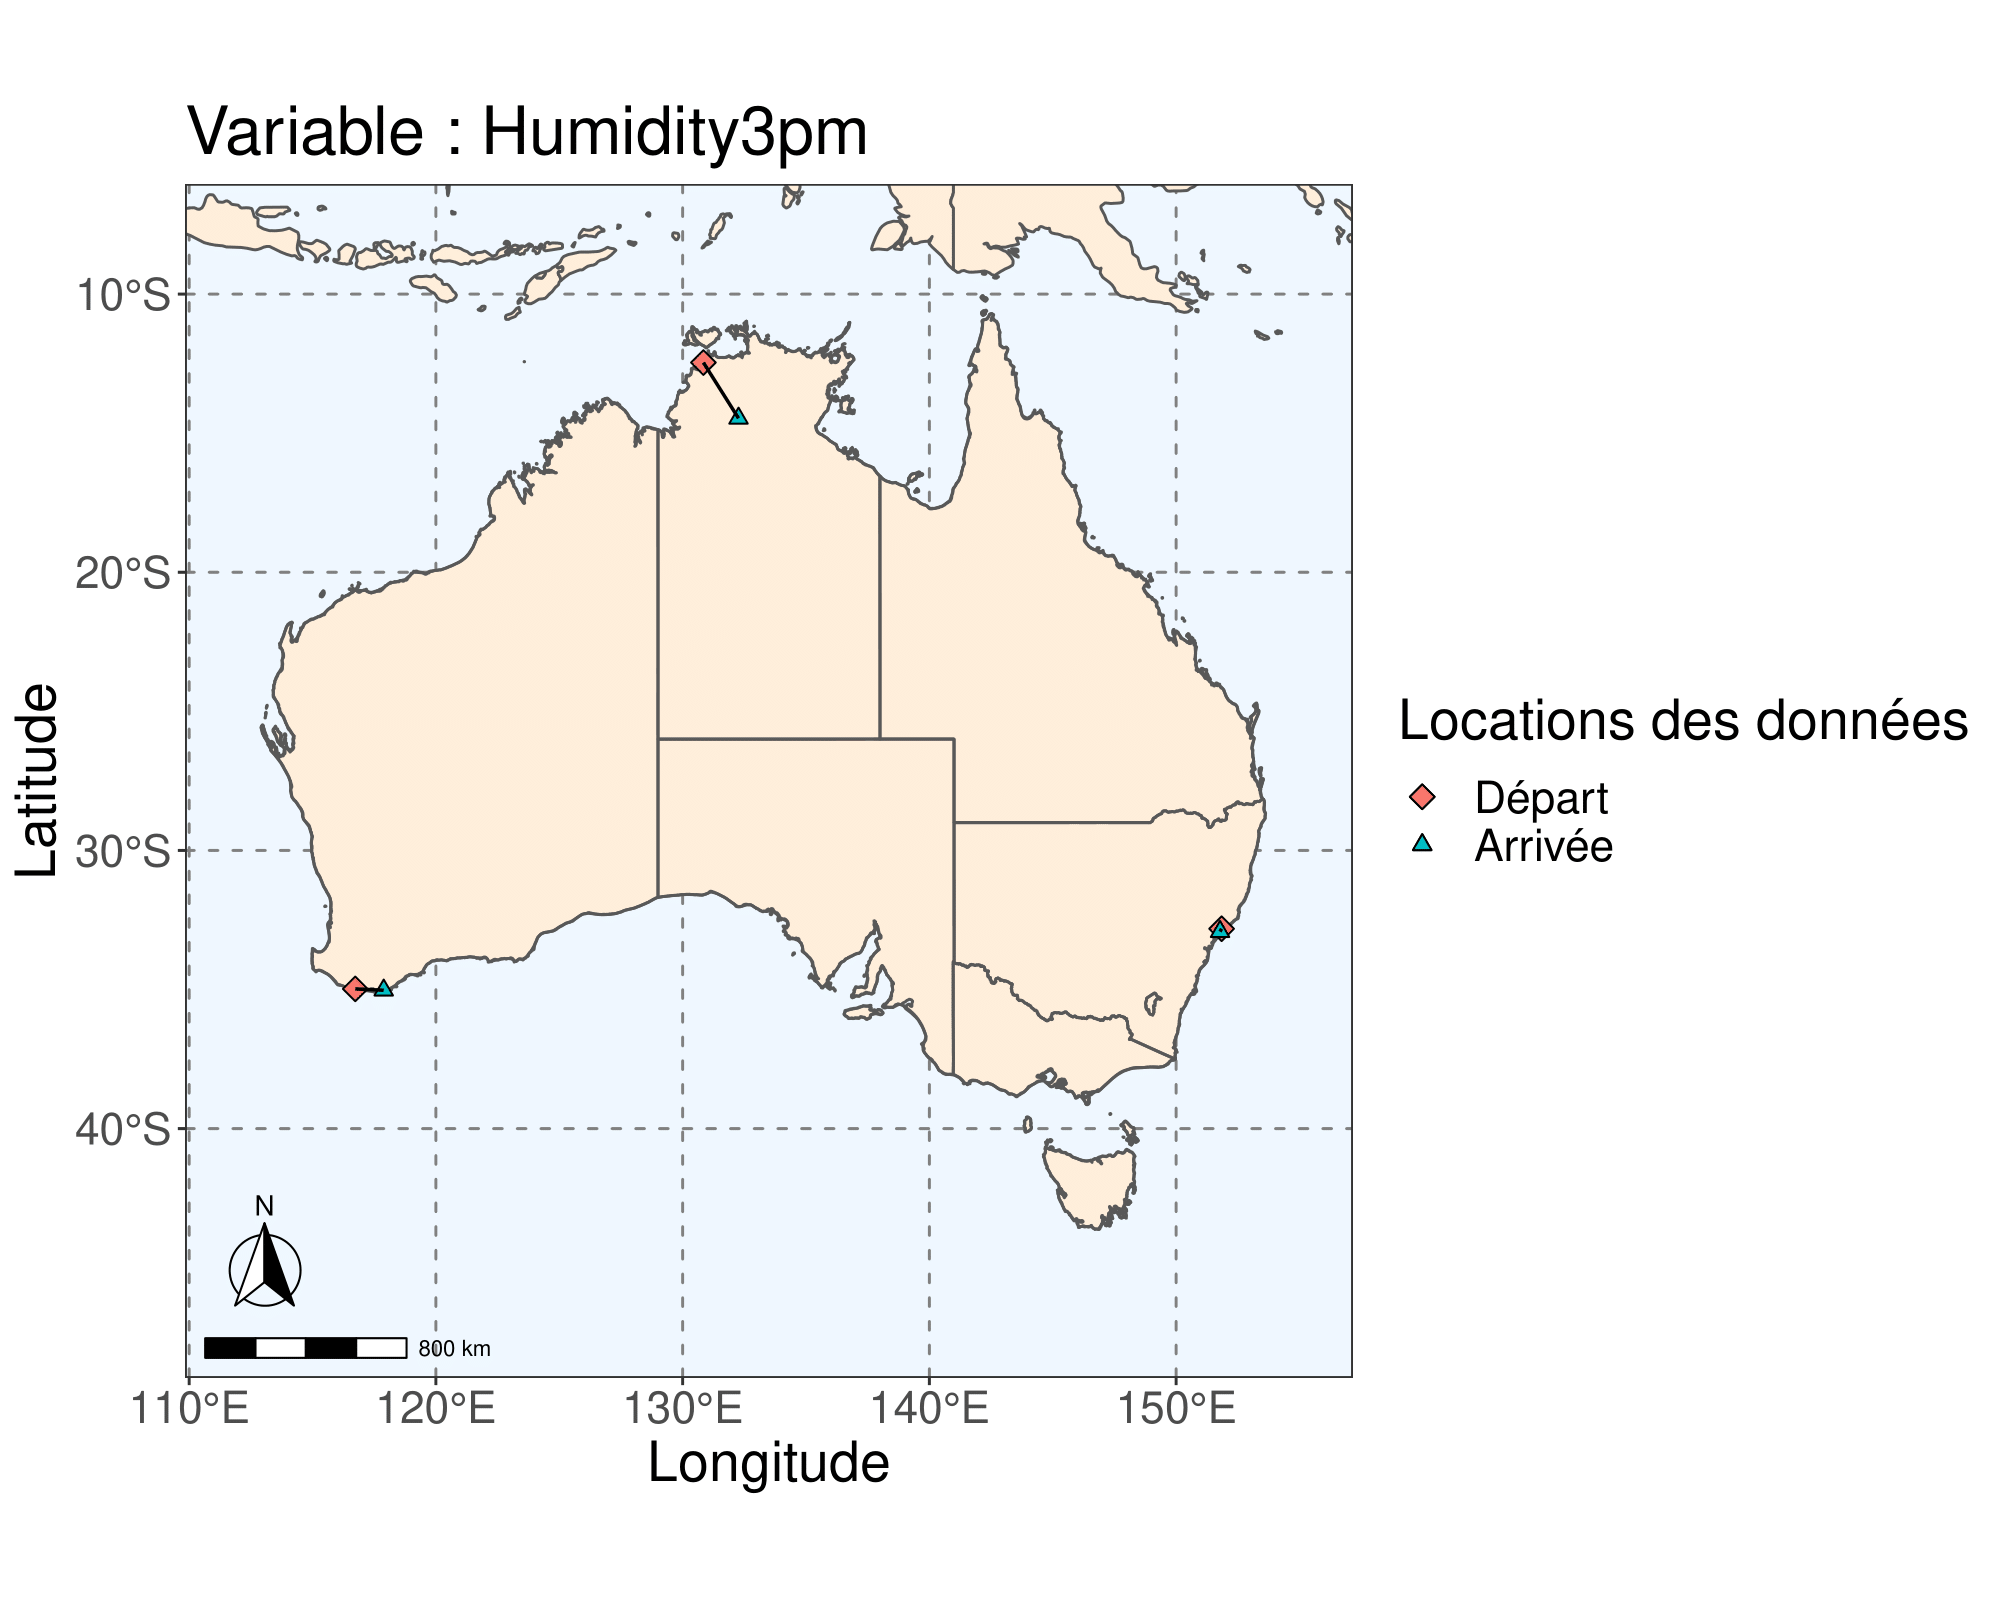
\includegraphics[width=0.45\textwidth]{Images/Australia_map_segments_complete/Australia_map_segments_complete-09.png}
    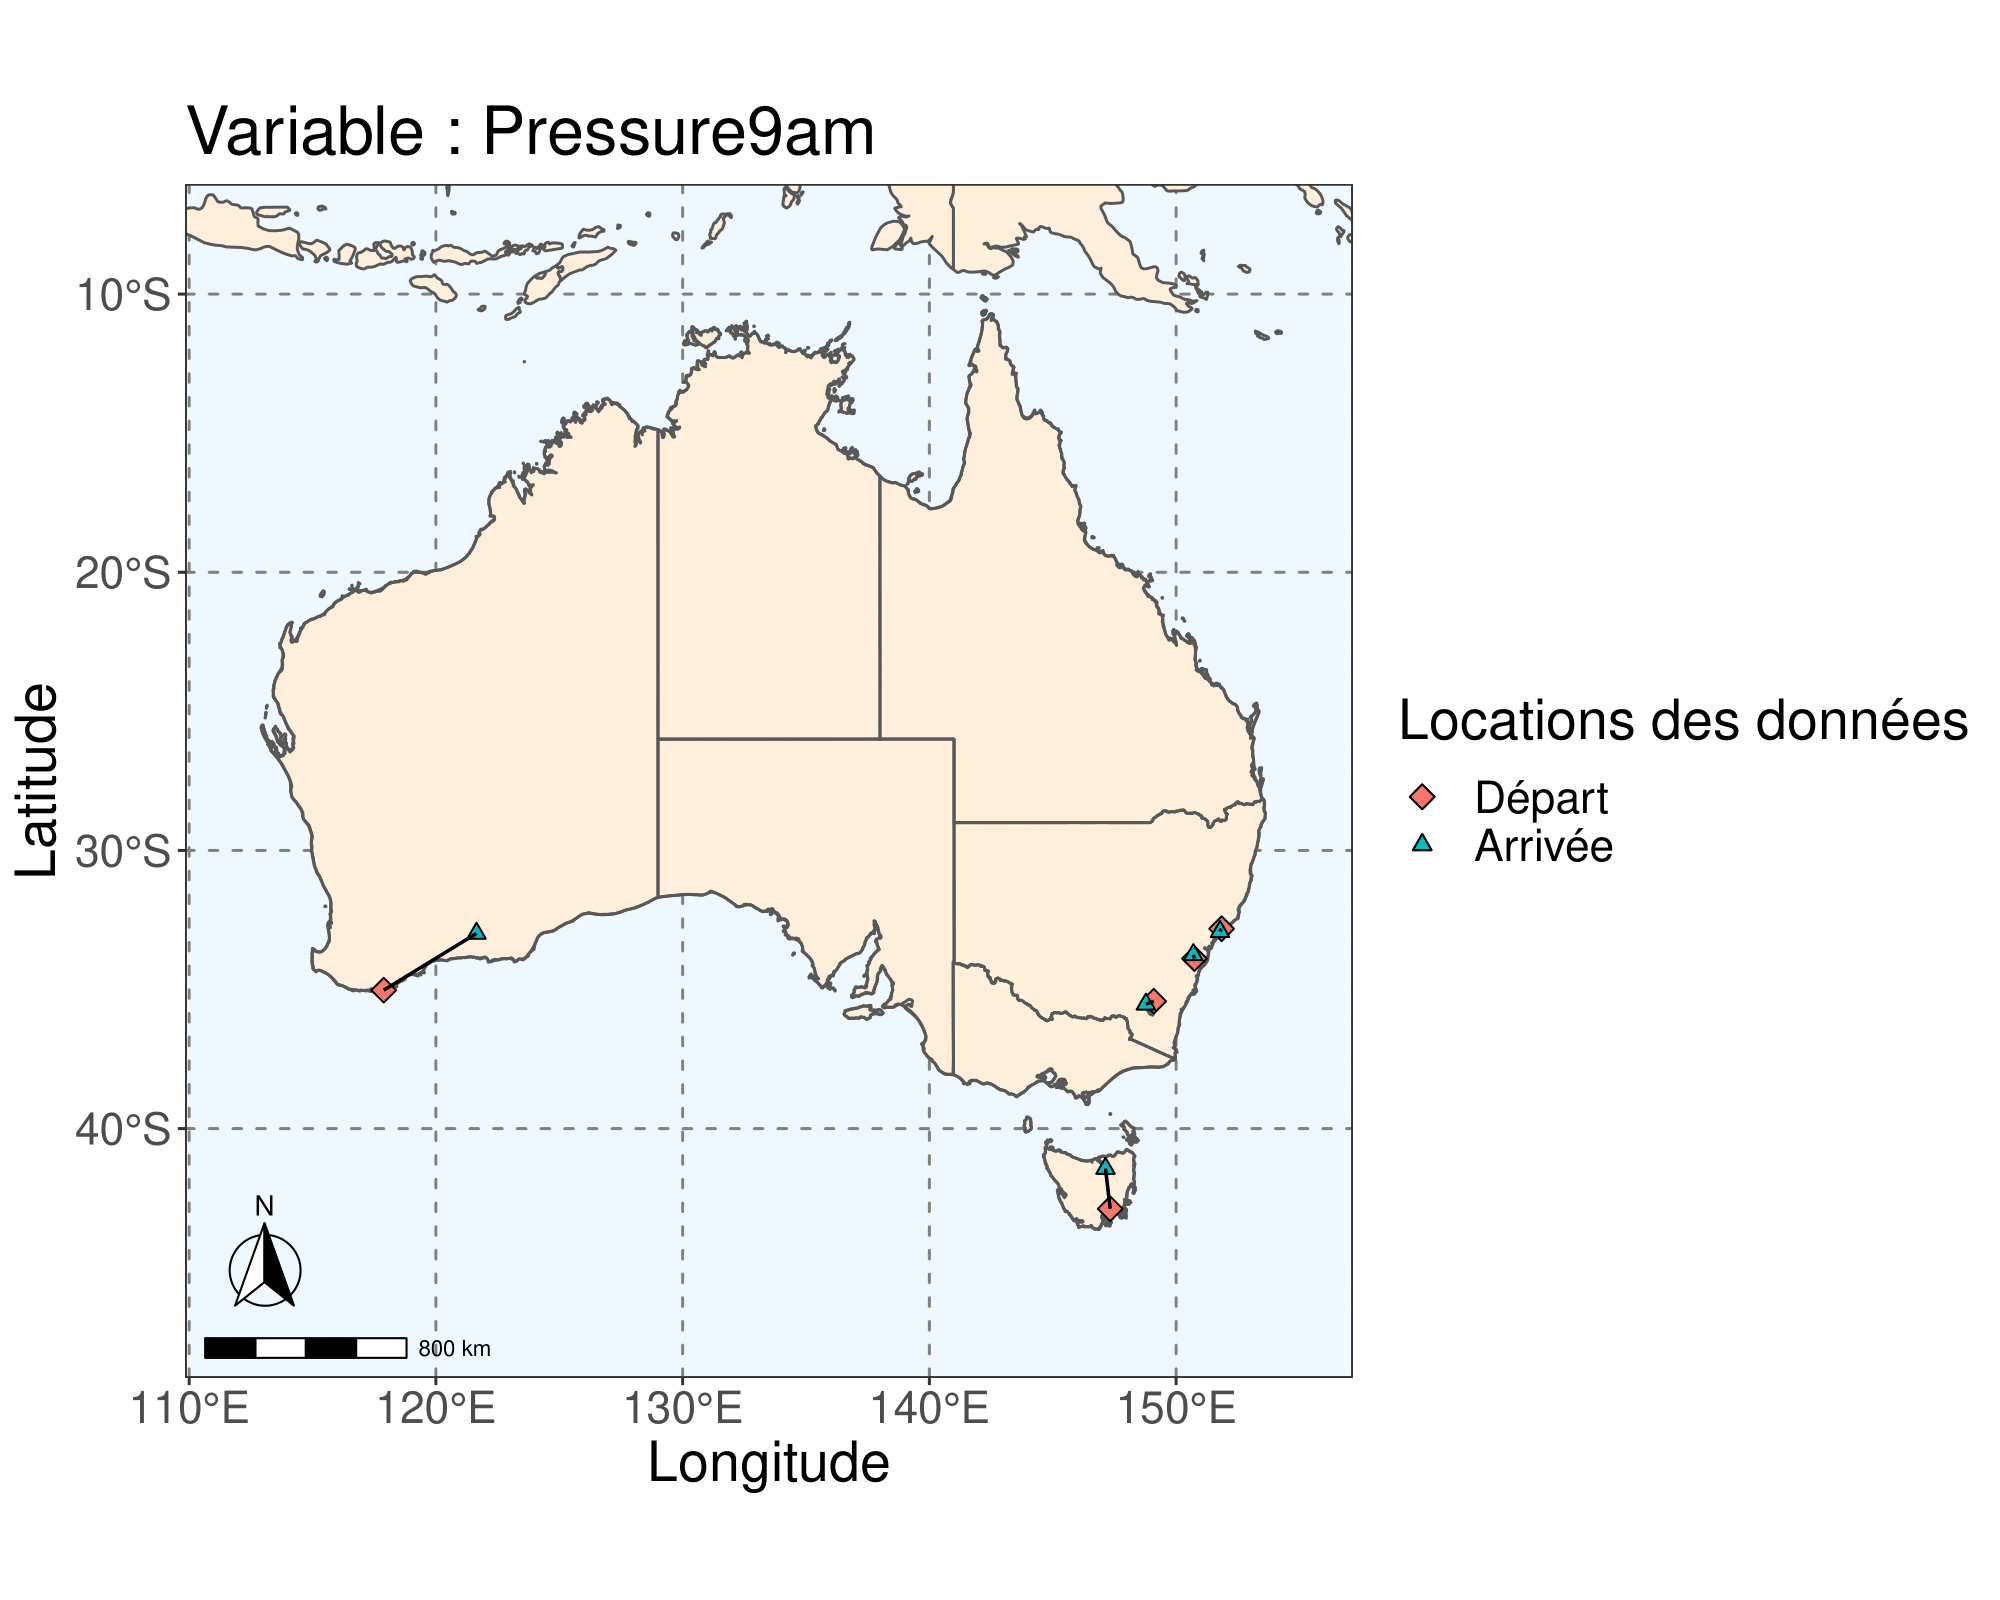
\includegraphics[width=0.45\textwidth]{Images/Australia_map_segments_complete/Australia_map_segments_complete-10.png}
    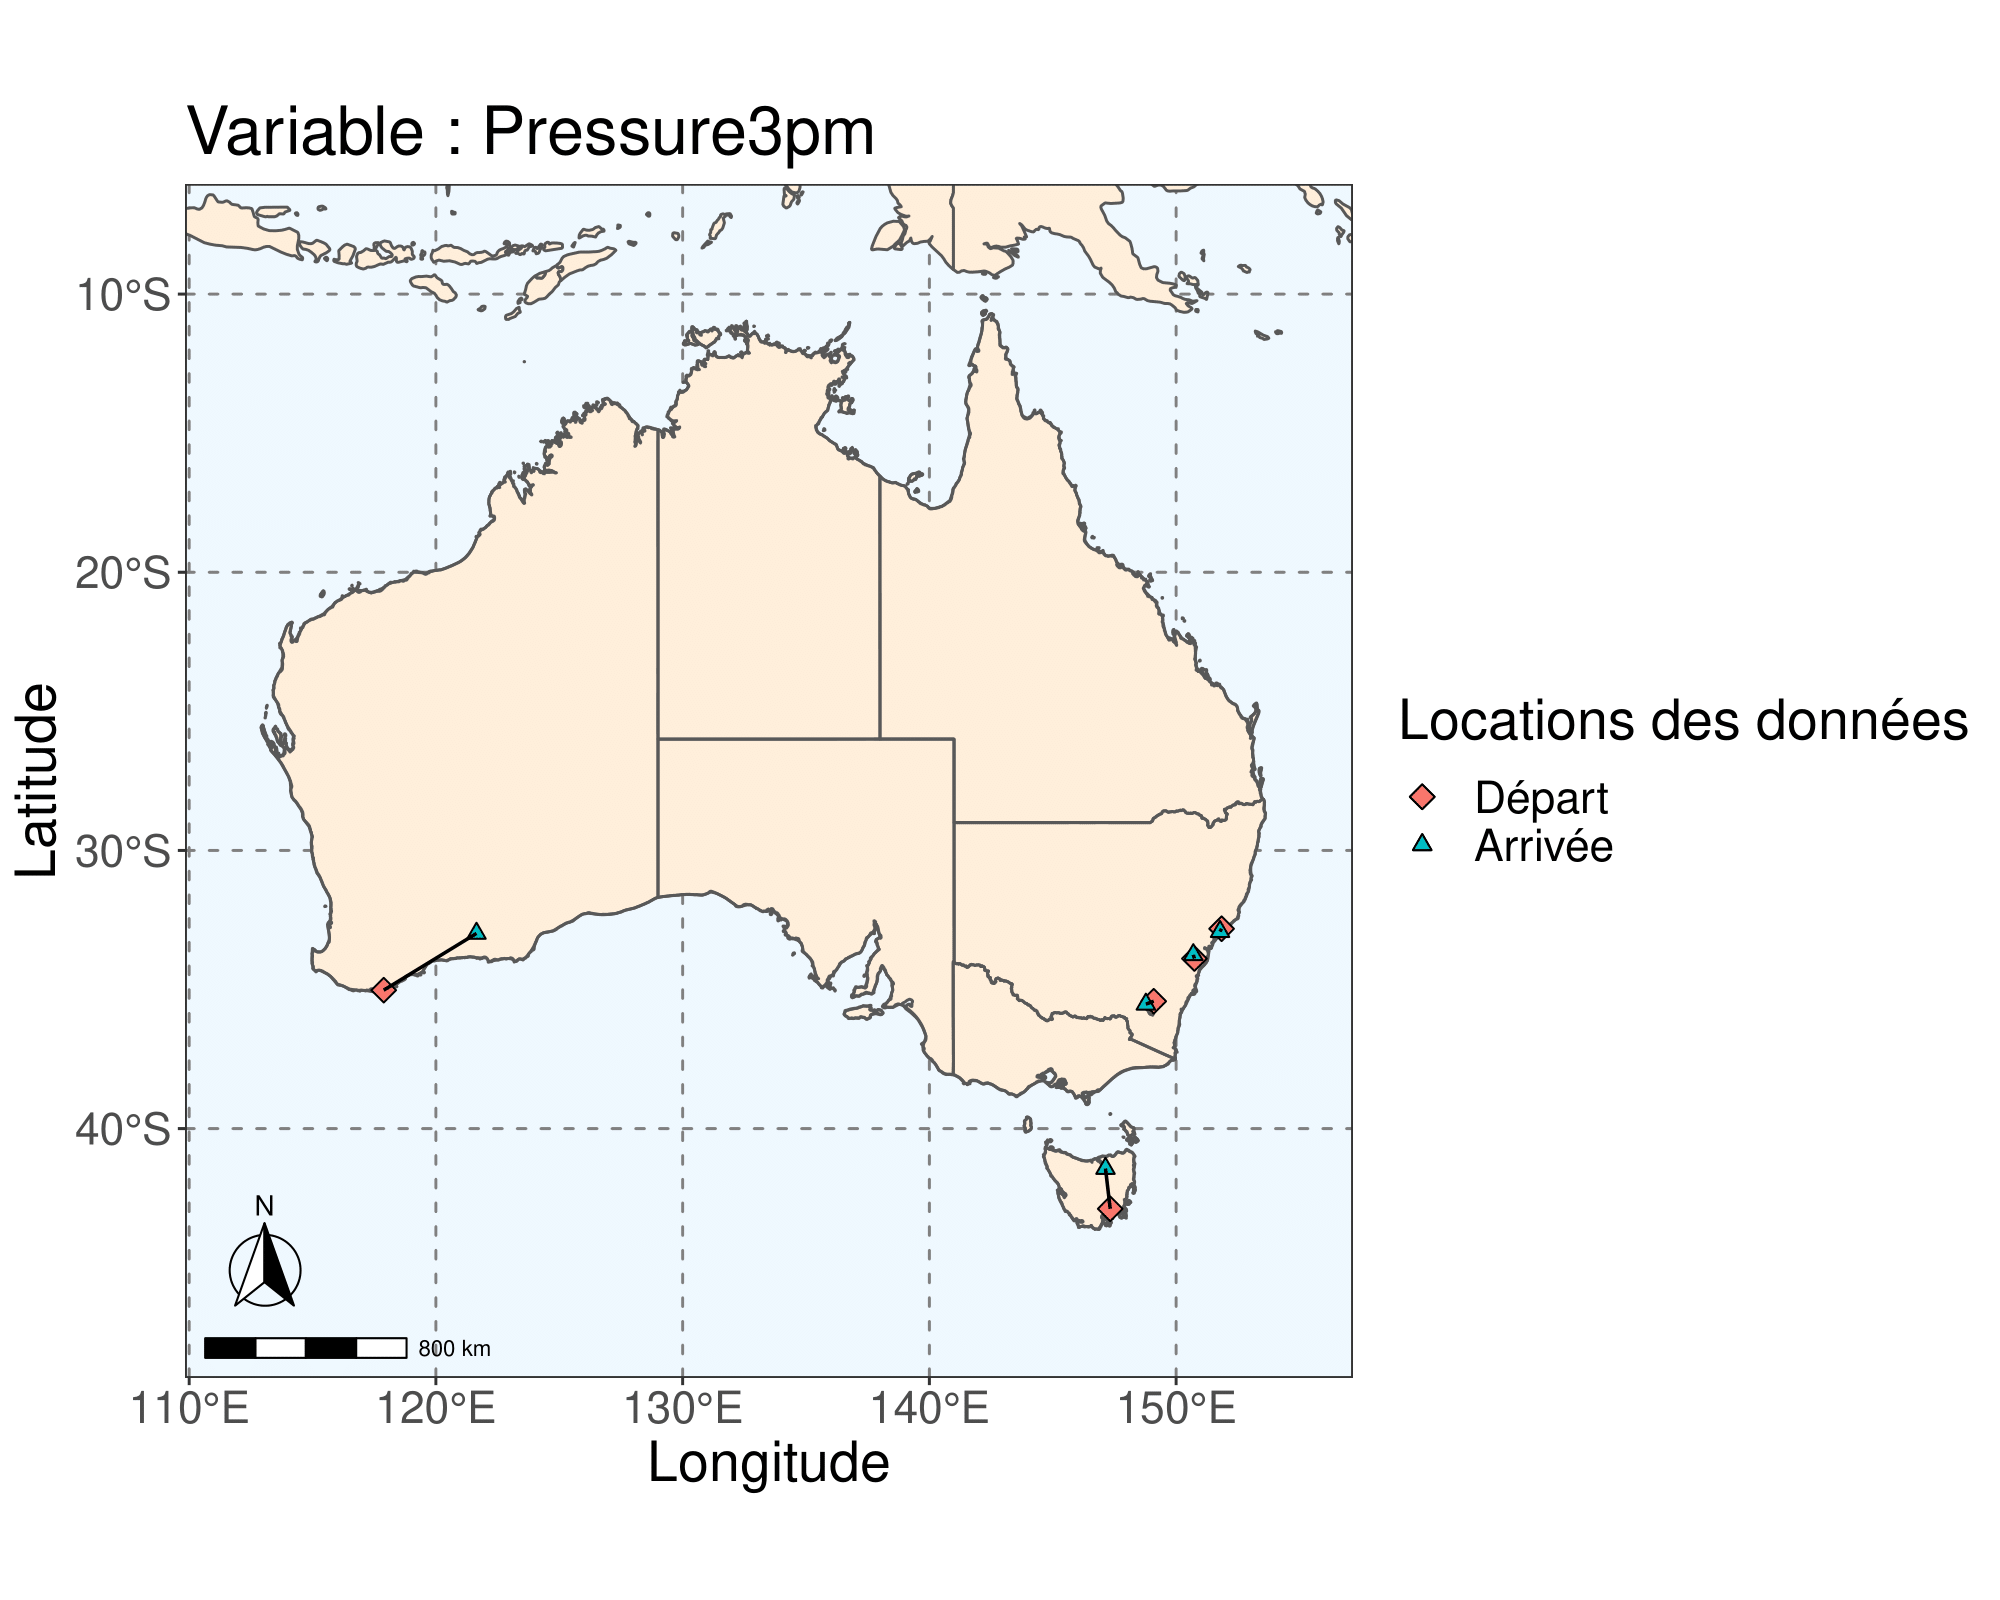
\includegraphics[width=0.45\textwidth]{Images/Australia_map_segments_complete/Australia_map_segments_complete-11.png}
    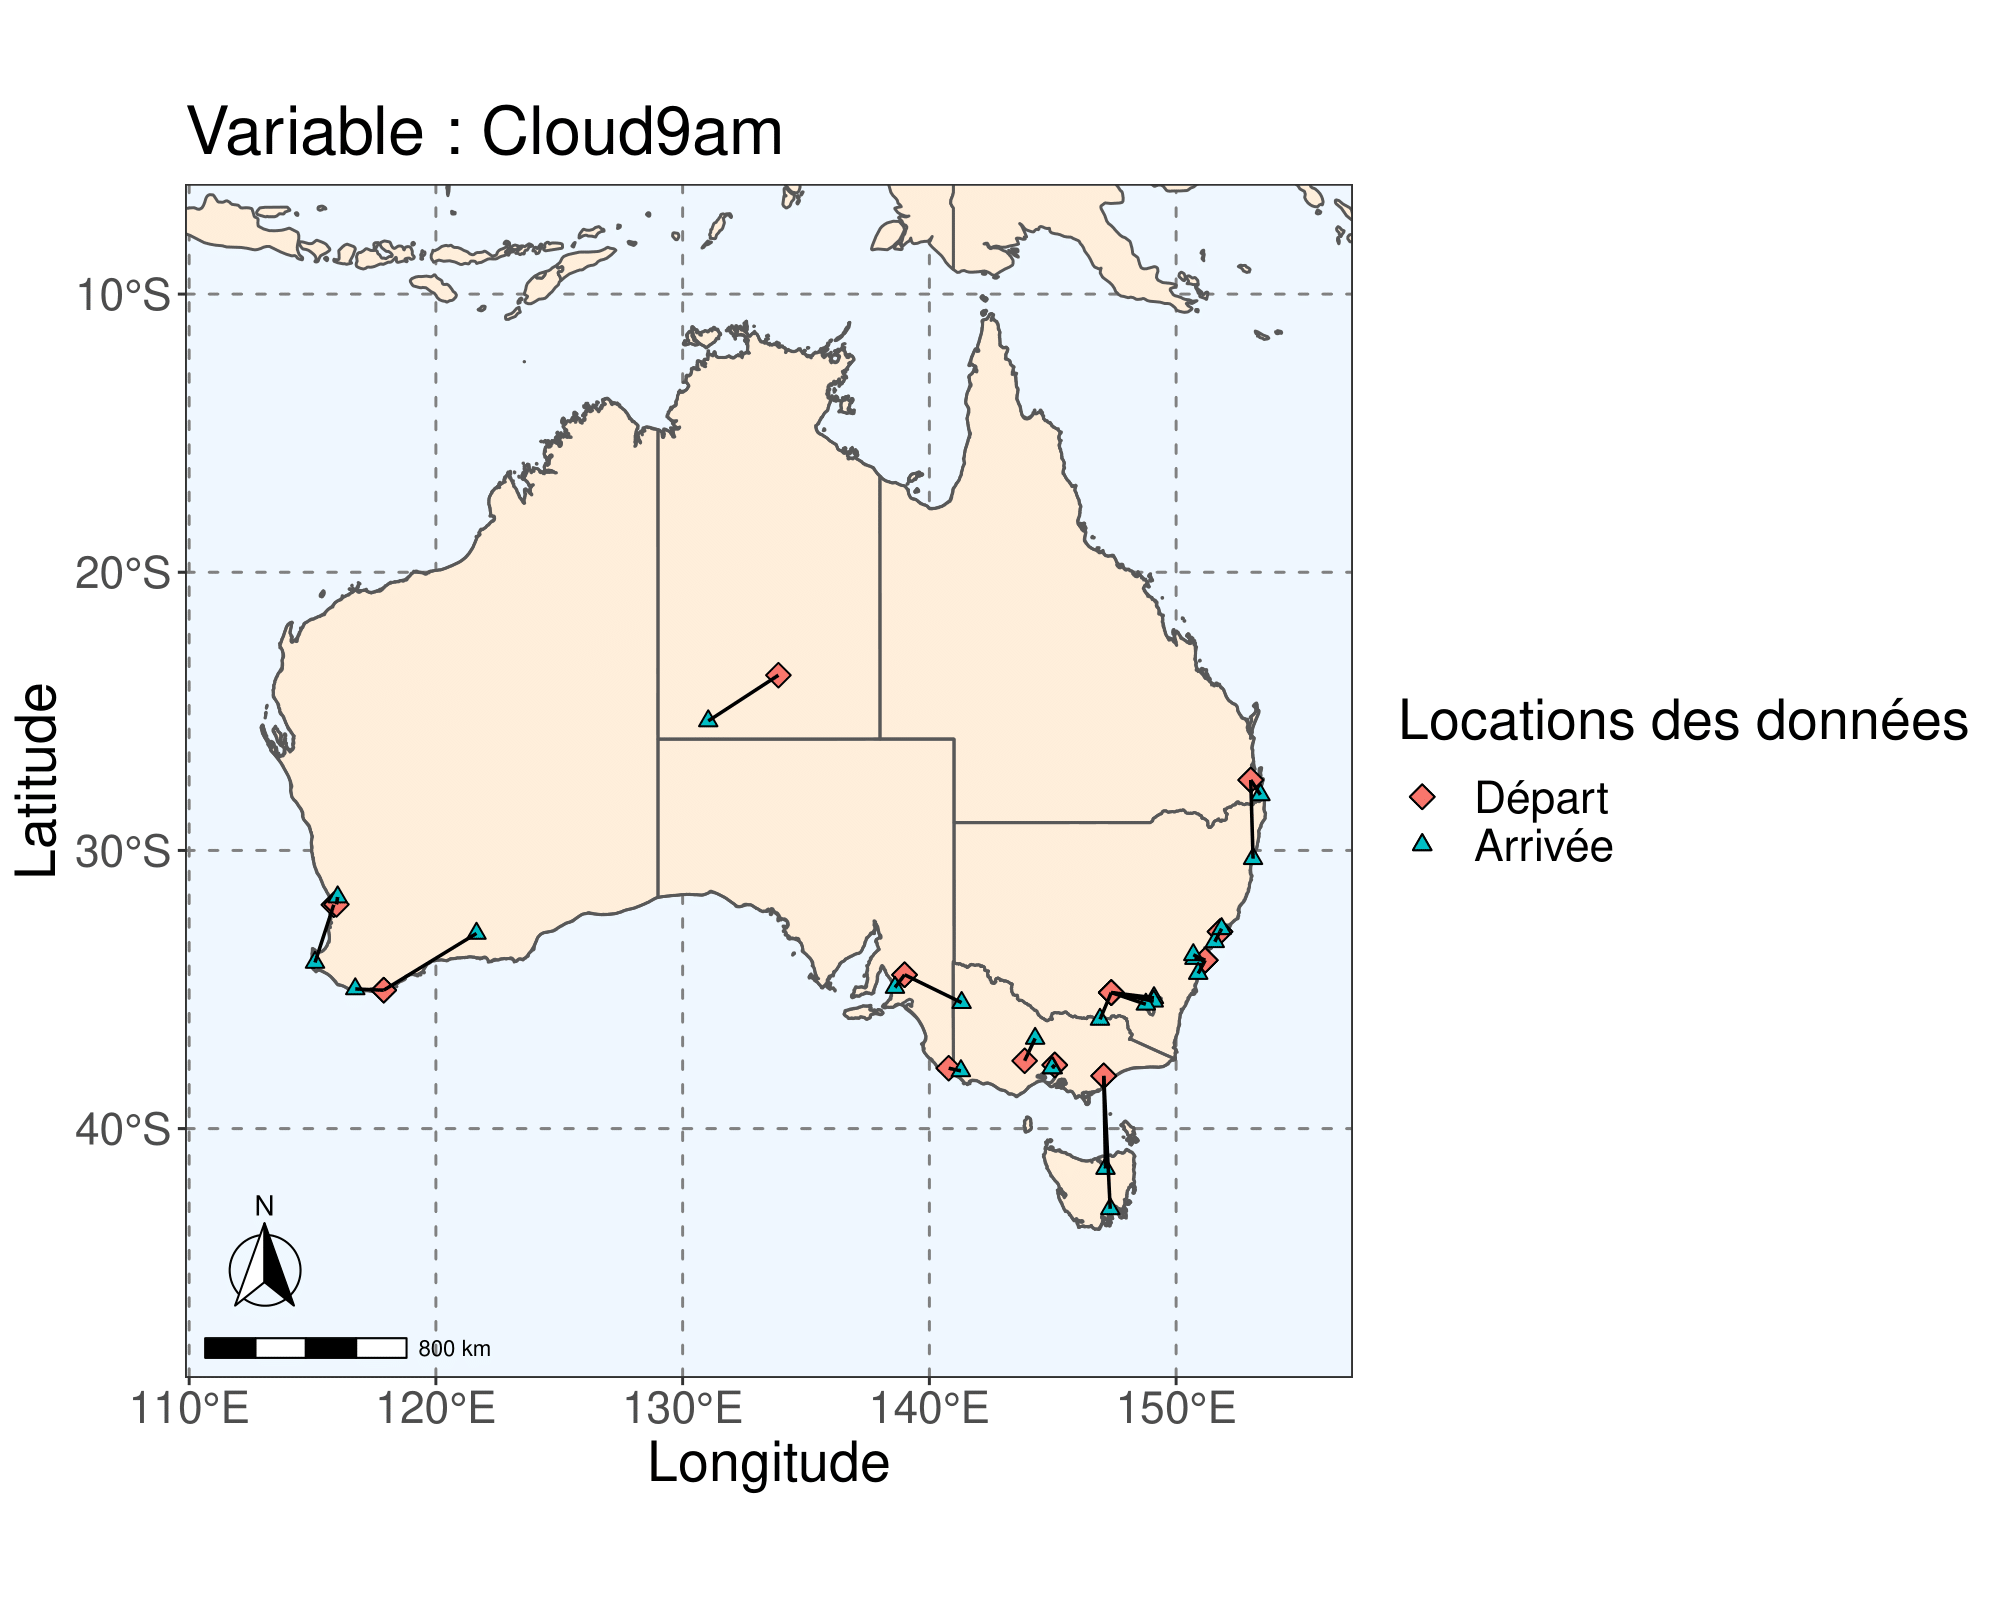
\includegraphics[width=0.45\textwidth]{Images/Australia_map_segments_complete/Australia_map_segments_complete-12.png}
    \caption{Chemin des observations copiées (ville de départ et ville(s) d'arrivée(s)) pour certaines des variables complétées 3/4.}
    \label{fig:path_data3}
\end{figure}
\begin{figure}[htp]
    \centering
    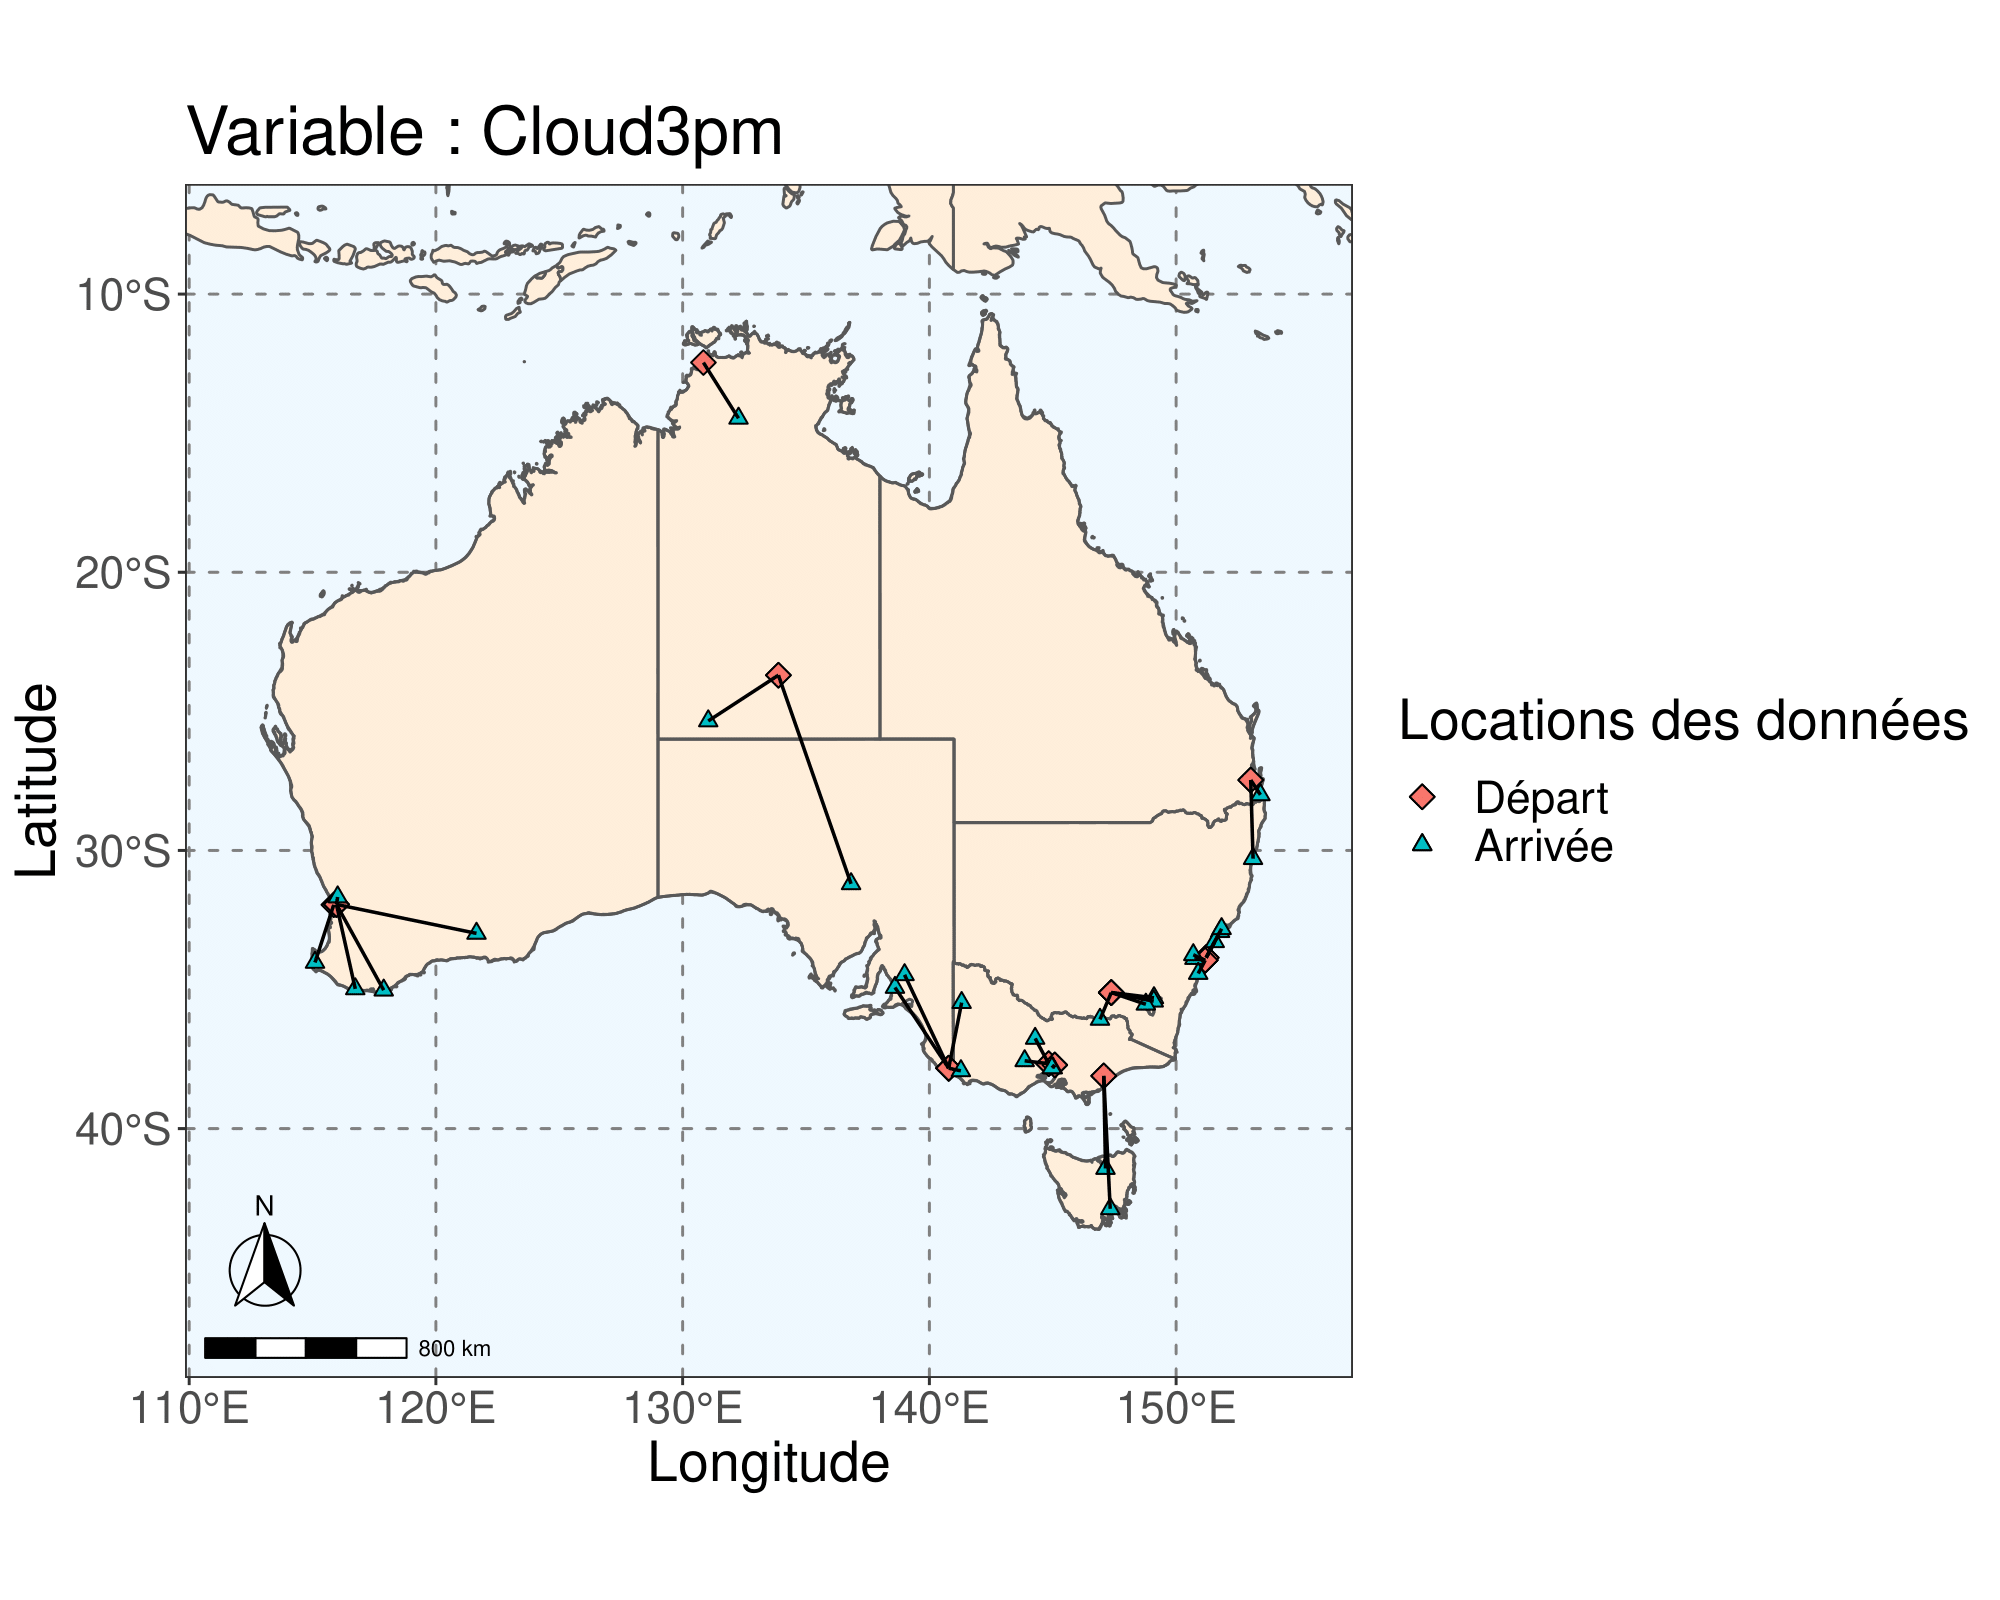
\includegraphics[width=0.45\textwidth]{Images/Australia_map_segments_complete/Australia_map_segments_complete-13.png}
    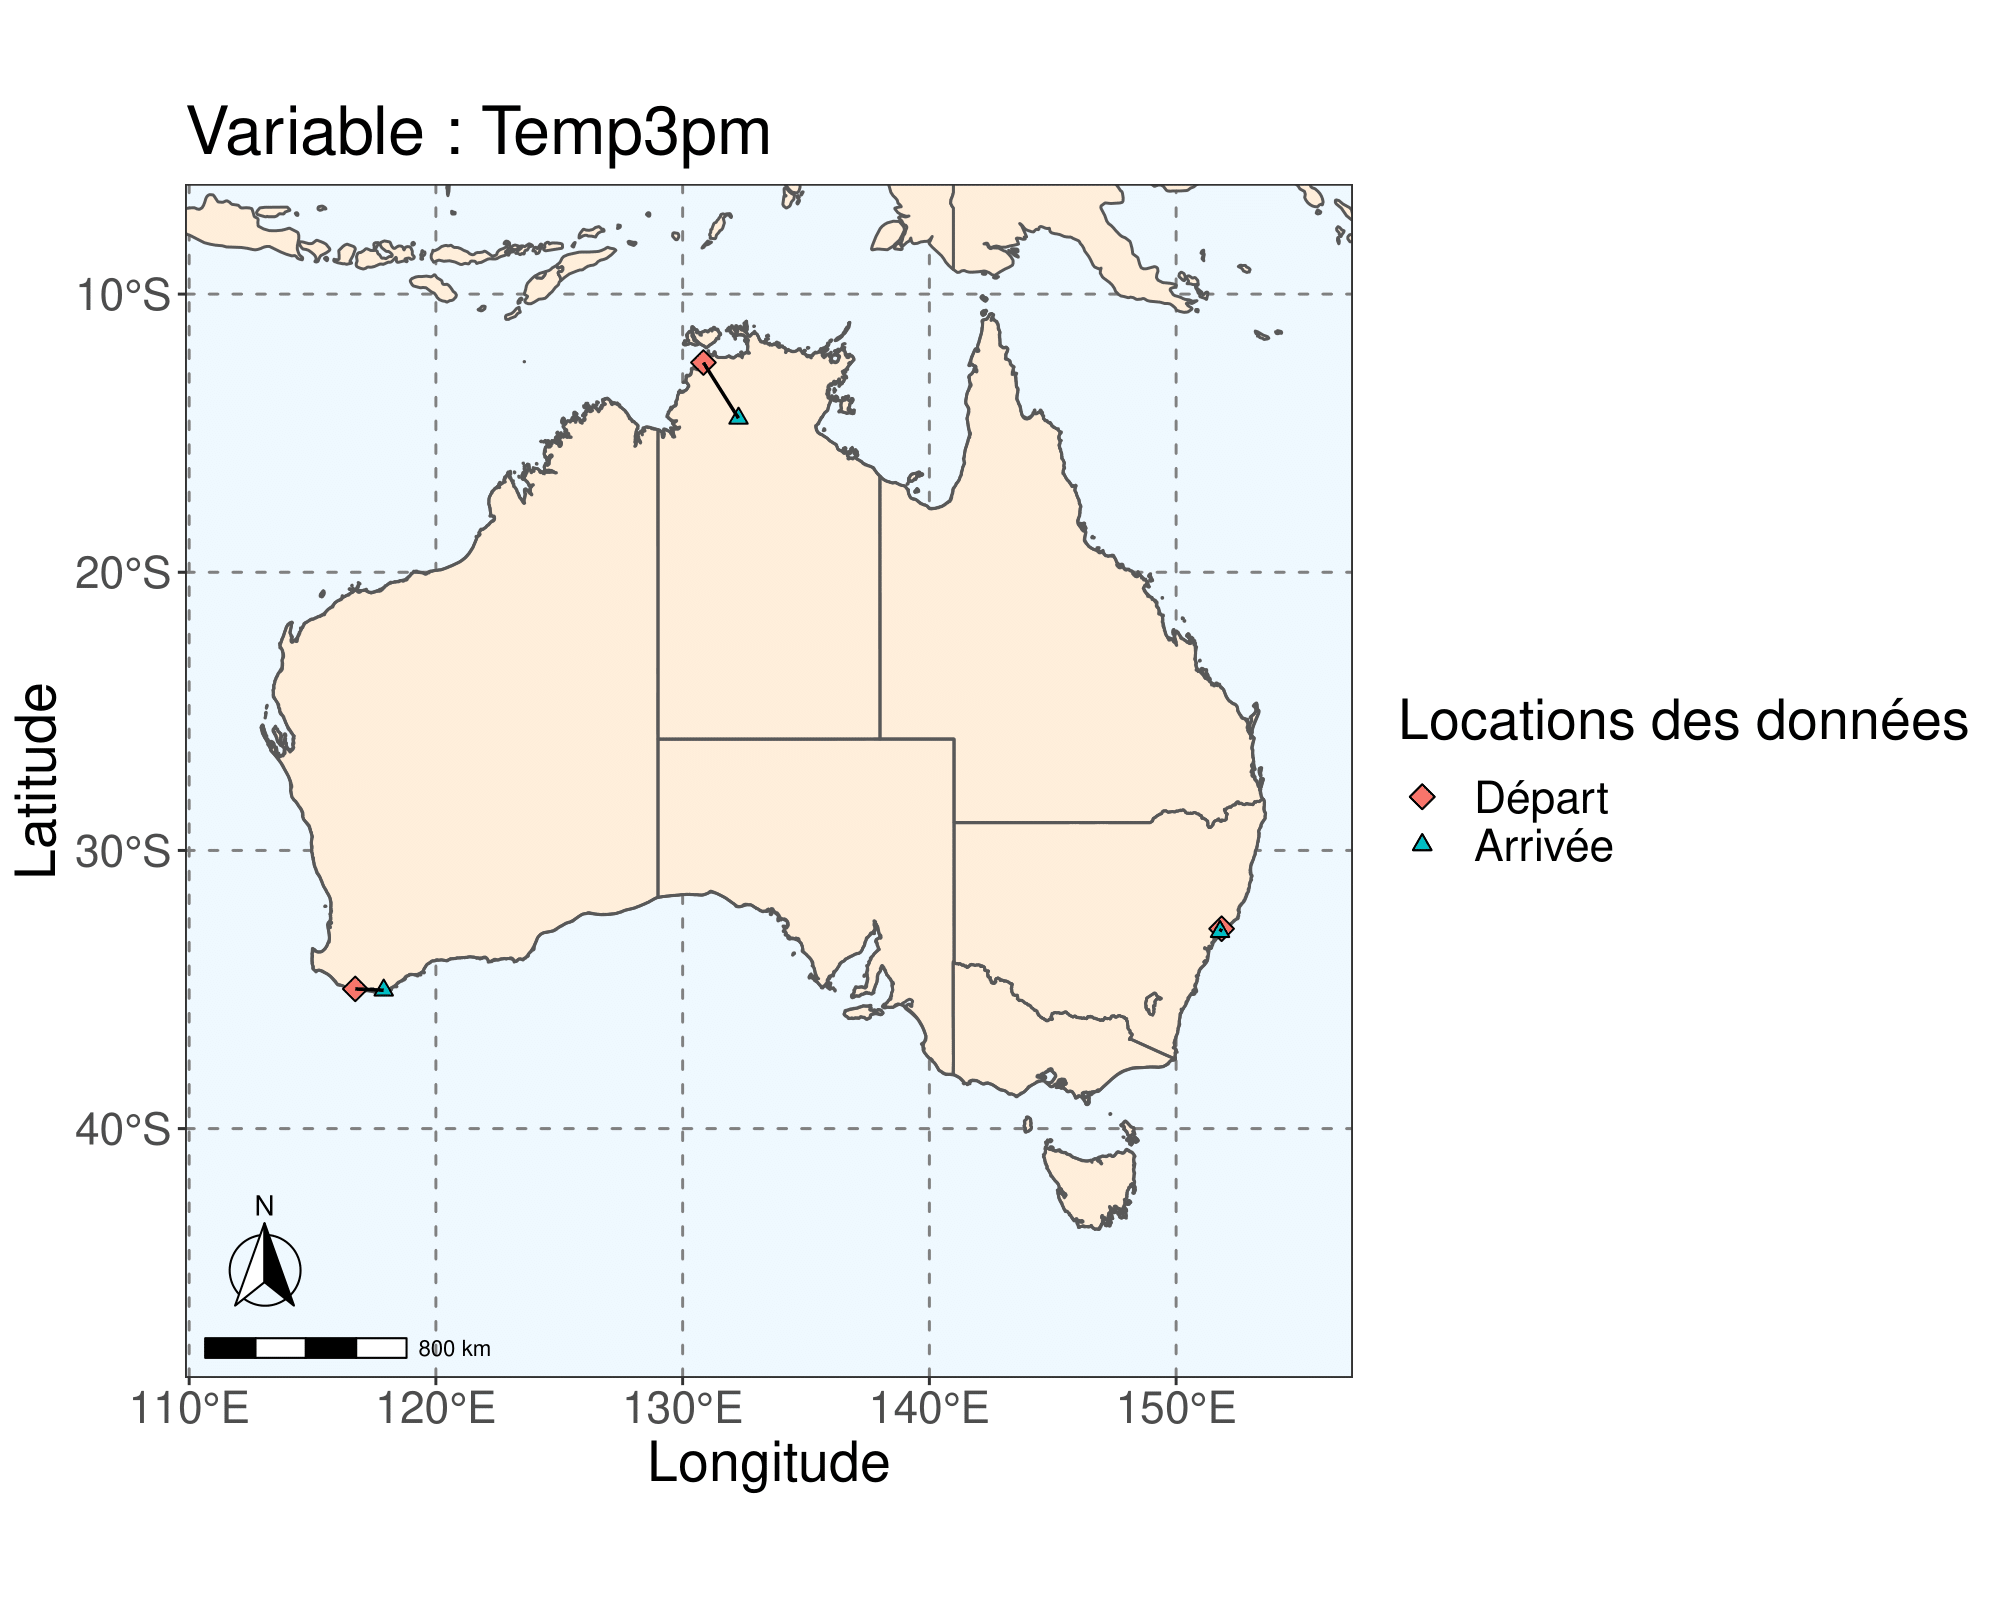
\includegraphics[width=0.45\textwidth]{Images/Australia_map_segments_complete/Australia_map_segments_complete-14.png}
    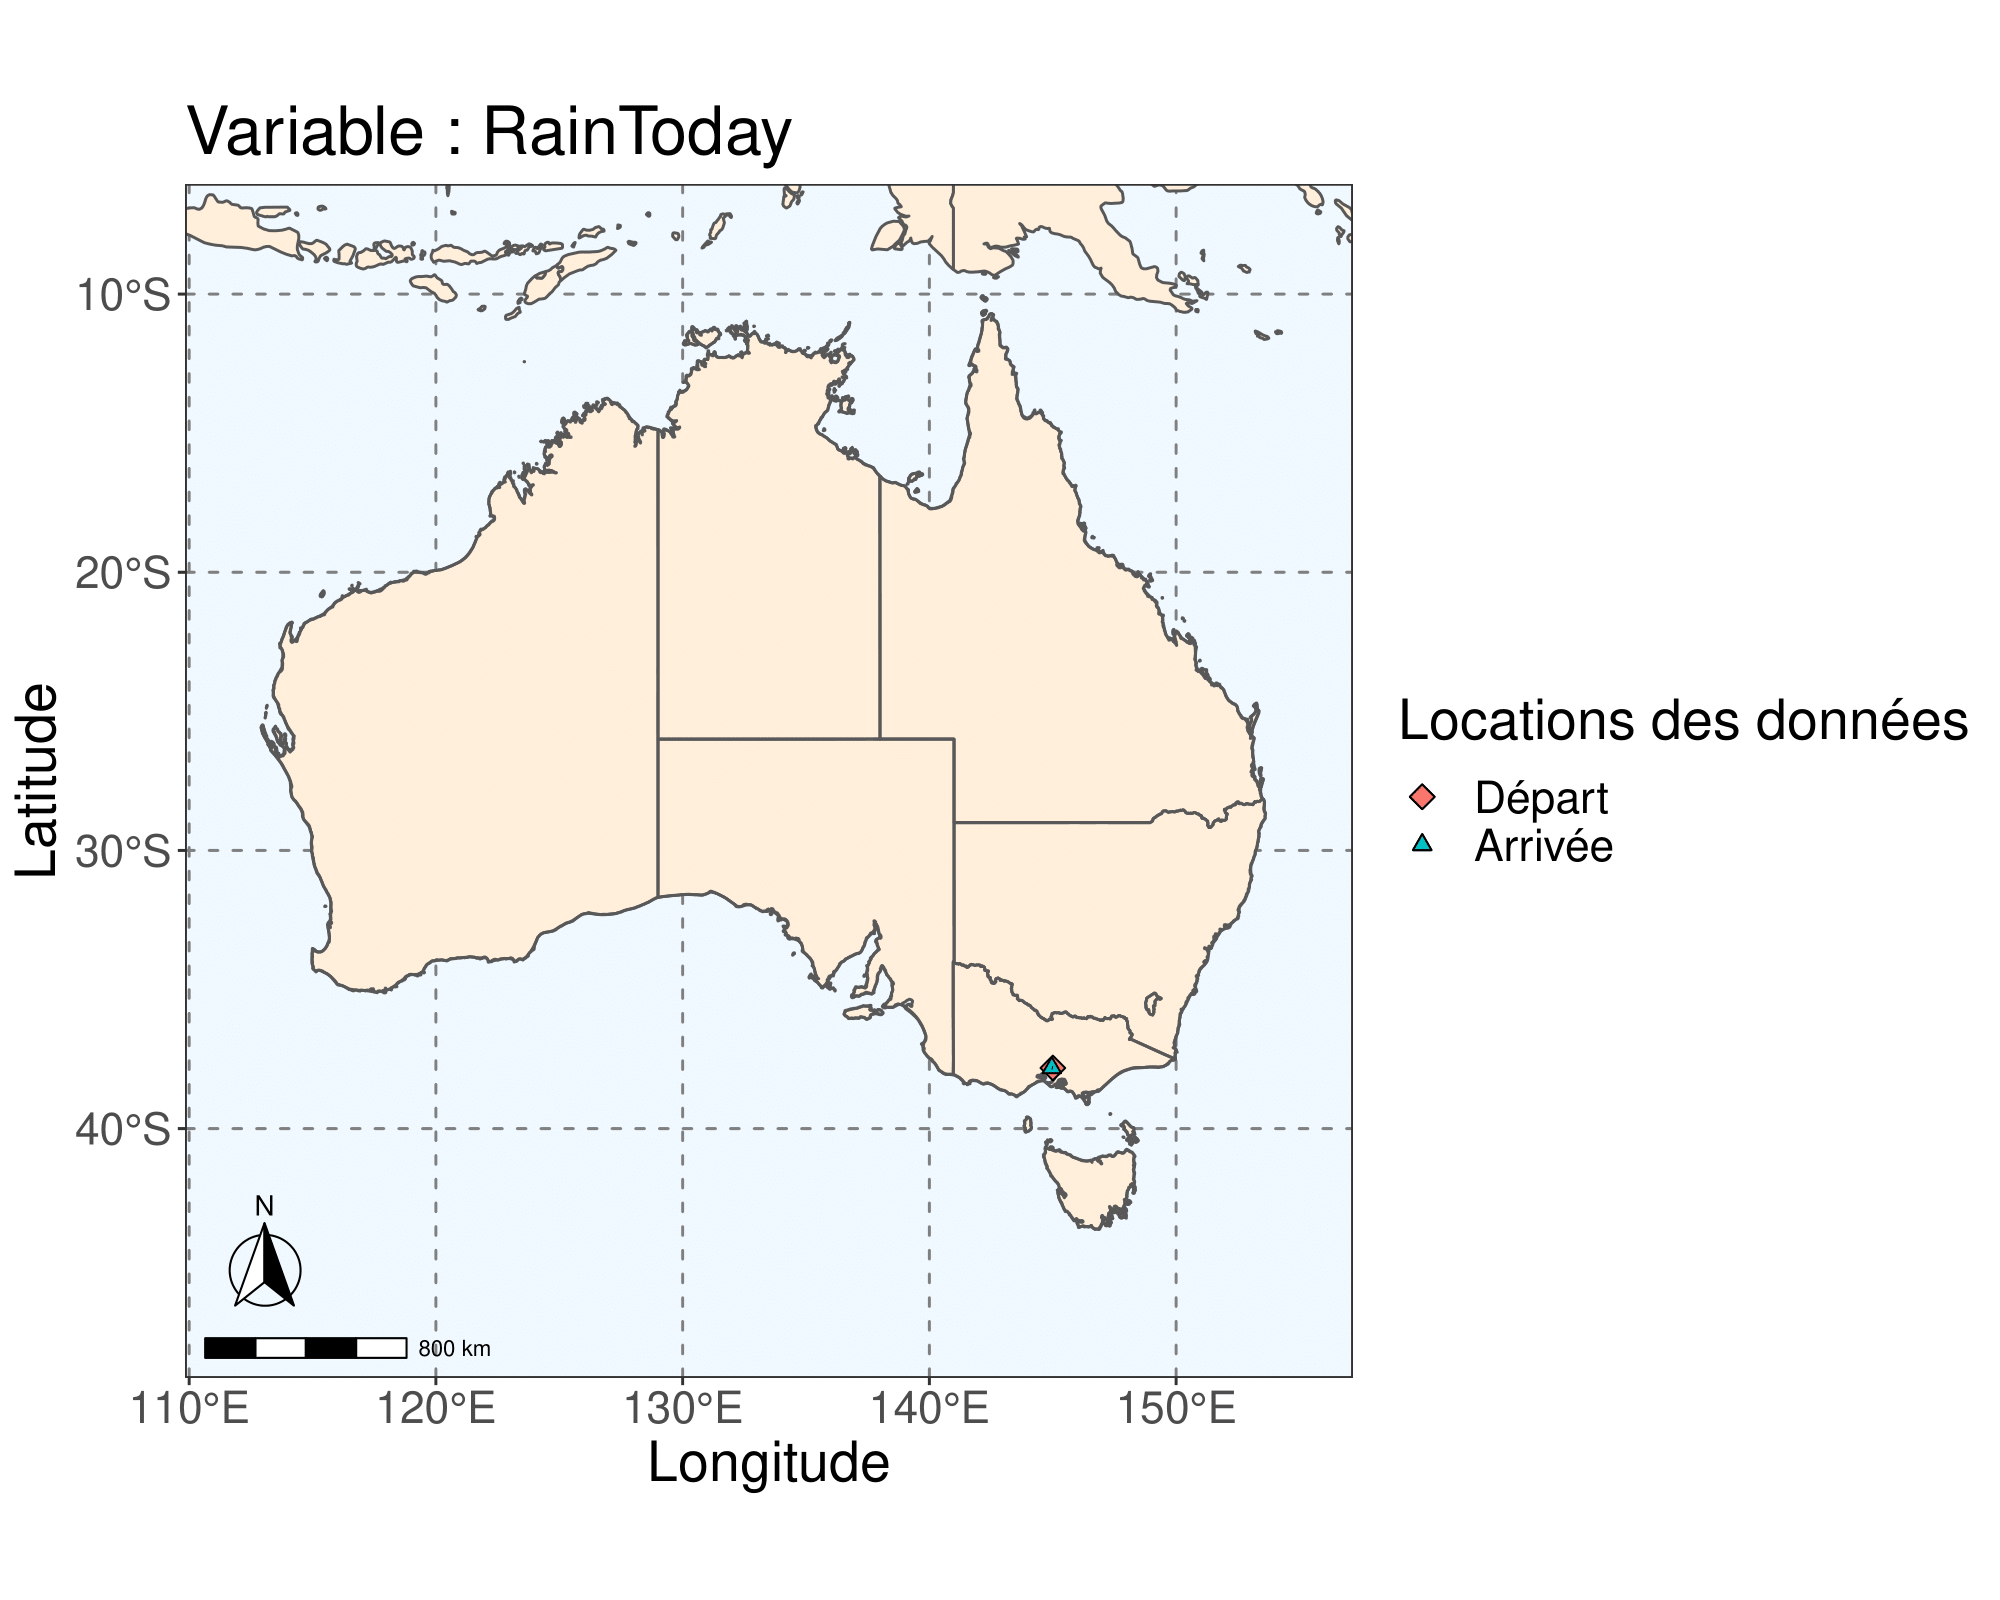
\includegraphics[width=0.45\textwidth]{Images/Australia_map_segments_complete/Australia_map_segments_complete-15.png}
    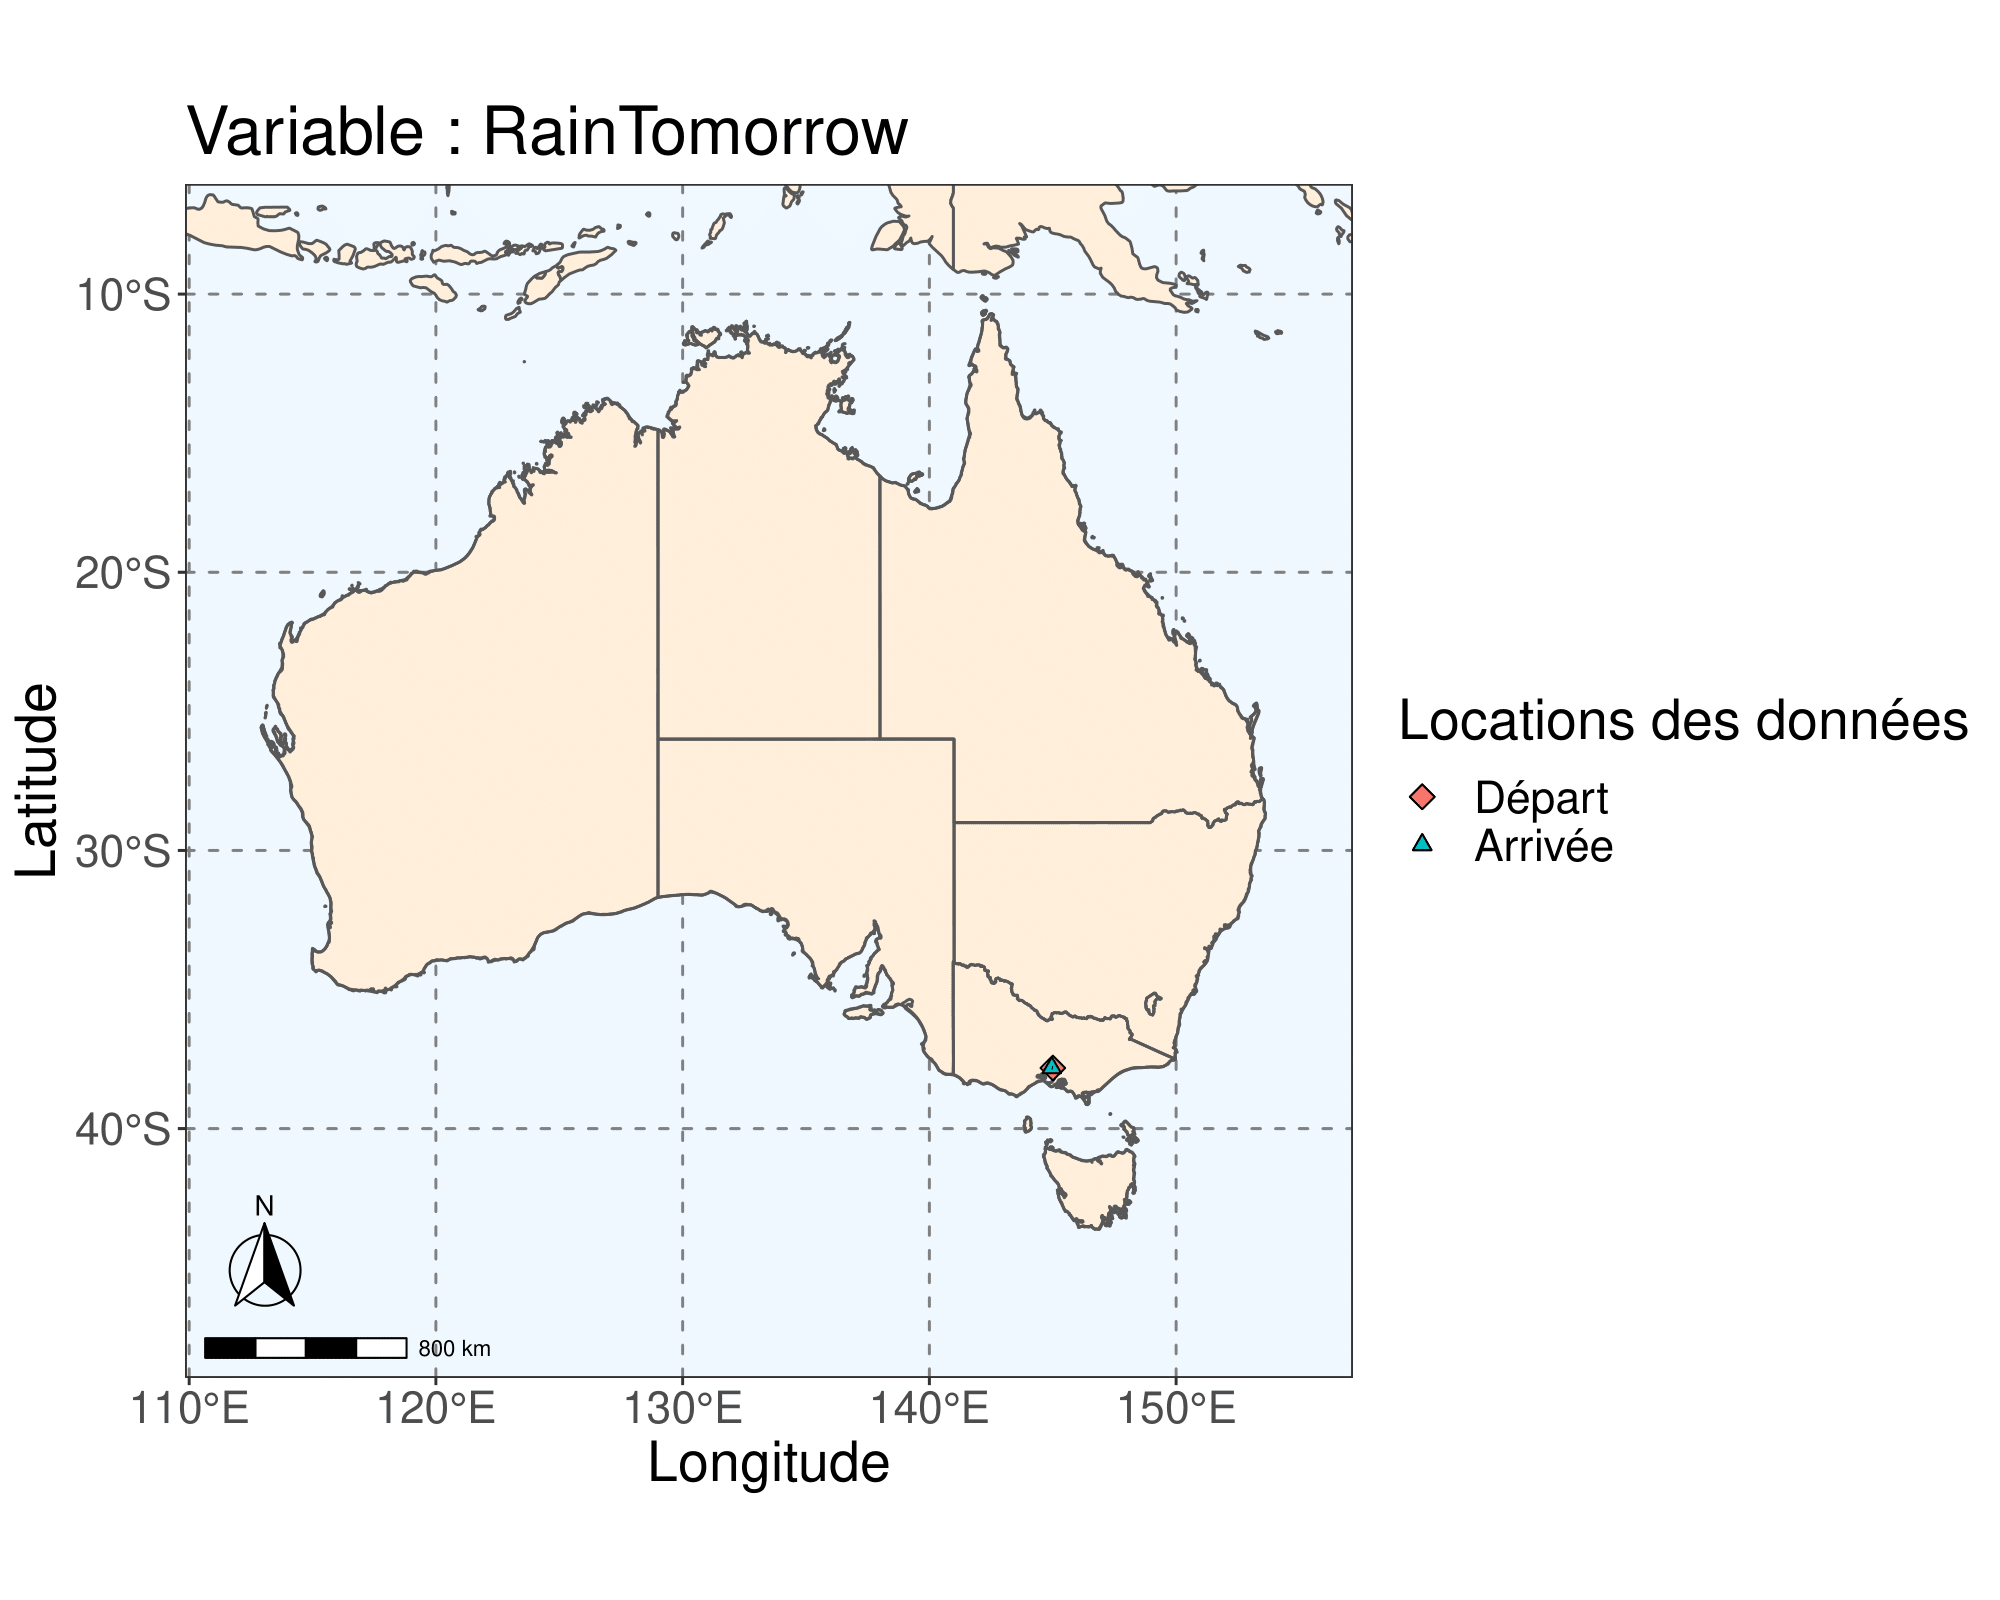
\includegraphics[width=0.45\textwidth]{Images/Australia_map_segments_complete/Australia_map_segments_complete-16.png}
    \caption{Chemin des observations copiées (ville de départ et ville(s) d'arrivée(s)) pour certaines des variables complétées 4/4.}
    \label{fig:path_data4}
\end{figure}
\end{document}
